\chapter{PENGUJIAN DAN ANALISIS}
\label{sec:chap4_pengujian}

\section{Pendahuluan Pengujian}
Bab ini membahas pengujian dan analisis terhadap sistem \textit{Credit Risk Scoring} berbasis \textit{Machine Learning Operations} (MLOps) yang telah dirancang pada Bab III. Pengujian tidak hanya diarahkan untuk melihat performa model prediktif, tetapi juga untuk memverifikasi kesiapan sistem sebagai pipeline operasional yang dapat melakukan pengolahan data, pelatihan model, interpretasi hasil, validasi kualitas data, penyajian model melalui API, serta pemantauan drift.

Ruang lingkup pengujian disusun agar mampu menjawab dua kebutuhan utama. Pertama, kebutuhan akademik, yaitu membuktikan bahwa metode yang digunakan memiliki dasar kuantitatif dan dapat dievaluasi secara ilmiah. Kedua, kebutuhan implementatif, yaitu membuktikan bahwa sistem dapat berjalan sebagai rangkaian proses MLOps yang mendukung reprodusibilitas, pelacakan eksperimen, dan pengambilan keputusan berbasis model. Dengan demikian, Bab IV berfungsi sebagai penghubung antara rancangan sistem dan bukti implementasi.

Secara umum, pengujian dilakukan melalui enam skenario utama, yaitu pengujian \textit{preprocessing} menggunakan WoE dan IV, penanganan ketidakseimbangan kelas menggunakan SMOTE, pelatihan dan \textit{hyperparameter tuning} model XGBoost, pengujian kualitas data sintetis menggunakan pendekatan TSTR dan TRTR, pengujian layanan inferensi FastAPI beserta aturan bisnis, serta pengujian deteksi drift dan pemicuan \textit{retraining} otomatis.

\section{Lingkungan Pengujian}
\label{sec:bab4_lingkungan_pengujian}
Pengujian dilakukan pada lingkungan komputasi yang dirancang untuk mendukung proses eksperimen pembelajaran mesin secara lokal. Spesifikasi perangkat keras dan perangkat lunak dicatat agar proses pengujian dapat direplikasi pada lingkungan lain dengan konfigurasi yang sebanding.

\begin{table}[H]
\centering
\caption{Spesifikasi perangkat keras pengujian}
\label{tab:bab4_hardware}
\begin{tabular}{|l|l|}
\hline
\textbf{Komponen} & \textbf{Spesifikasi} \\
\hline
Prosesor & Intel Core i7 / AMD Ryzen 7, minimal 4 \textit{core} dan 8 \textit{thread} \\
\hline
Memori utama & 16 GB DDR4 \\
\hline
Penyimpanan & SSD 512 GB NVMe PCIe \\
\hline
Arsitektur sistem & x64-based processor \\
\hline
\end{tabular}
\end{table}

\begin{table}[H]
\centering
\caption{Spesifikasi perangkat lunak pengujian}
\label{tab:bab4_software}
\begin{tabular}{|l|l|}
\hline
\textbf{Komponen} & \textbf{Perangkat Lunak} \\
\hline
Sistem operasi & Microsoft Windows 11 Home / Pro x64 \\
\hline
Bahasa pemrograman & Python 3.10.x / 3.11.x \\
\hline
Web API & FastAPI dan Uvicorn \\
\hline
Machine learning & XGBoost, Scikit-Learn, Imbalanced-Learn \\
\hline
Pelacakan eksperimen & MLflow \\
\hline
Interpretabilitas & SHAP \\
\hline
Otomasi dan kontainerisasi & n8n, Docker, dan Docker Compose \\
\hline
\end{tabular}
\end{table}

Lingkungan tersebut dipilih karena mencerminkan kebutuhan minimum untuk menjalankan eksperimen data tabular, melakukan tuning model, menyimpan artefak eksperimen, serta menjalankan layanan inferensi berbasis API. Penggunaan Docker dan n8n juga mendukung simulasi otomasi MLOps yang lebih dekat dengan lingkungan operasional.

\section{Skenario Pengujian}
\label{sec:bab4_skenario_pengujian}
Skenario pengujian dirancang untuk mencakup seluruh siklus hidup sistem, mulai dari data mentah hingga pemantauan model setelah model digunakan. Rangkuman skenario pengujian ditunjukkan pada Tabel \ref{tab:bab4_skenario}.

\begin{table}[H]
\centering
\caption{Skenario pengujian sistem}
\label{tab:bab4_skenario}
\begin{tabular}{|p{0.05\textwidth}|p{0.31\textwidth}|p{0.52\textwidth}|}
\hline
\textbf{No.} & \textbf{Skenario} & \textbf{Tujuan Pengujian} \\
\hline
1 & Preprocessing WoE dan IV & Menguji efektivitas transformasi fitur serta seleksi fitur berdasarkan kekuatan prediktif. \\
\hline
2 & Penanganan imbalance dengan SMOTE & Memastikan data latih menjadi lebih seimbang sehingga model tidak bias terhadap kelas mayoritas. \\
\hline
3 & Pelatihan dan tuning XGBoost & Menentukan konfigurasi model terbaik berdasarkan performa validasi dan evaluasi data uji. \\
\hline
4 & Quality gate data sintetis & Menguji utilitas data sintetis dan risiko kebocoran privasi melalui metrik TSTR, TRTR, DCR, dan KS. \\
\hline
5 & API serving dan aturan bisnis & Memverifikasi layanan prediksi FastAPI, penerapan aturan usia, database, dan konfirmasi email HITL. \\
\hline
6 & Drift dan retraining otomatis & Menguji deteksi perubahan distribusi data dan pemicuan webhook n8n untuk retraining. \\
\hline
7 & Studi ablasi perbandingan model & Mengukur kontribusi transformasi WoE dan SMOTE pada beberapa arsitektur model. \\
\hline
\end{tabular}
\end{table}

Pembagian skenario ini memperlihatkan bahwa pengujian tidak berhenti pada akurasi model. Sistem juga diuji dari sisi kualitas data, keamanan penggunaan data sintetis, ketahanan aturan bisnis, serta kesiapan pemantauan model setelah deployment.

Sebagai gambaran menyeluruh terhadap cakupan fungsi yang diuji, diagram use case sistem ditunjukkan pada Gambar \ref{fig:bab4_use_case_diagram}. Diagram tersebut memperlihatkan interaksi antara pengguna, analis atau pihak penanggung jawab persetujuan, layanan prediksi, orkestrasi n8n, serta komponen pendukung seperti ingestion dokumen, pengiriman konfirmasi, monitoring drift, dan retraining. Dengan demikian, diagram ini menjadi penghubung antara skenario pengujian pada Bab IV dan implementasi pipeline MLOps yang telah dirancang pada Bab III.

\begin{figure}[H]
\centering
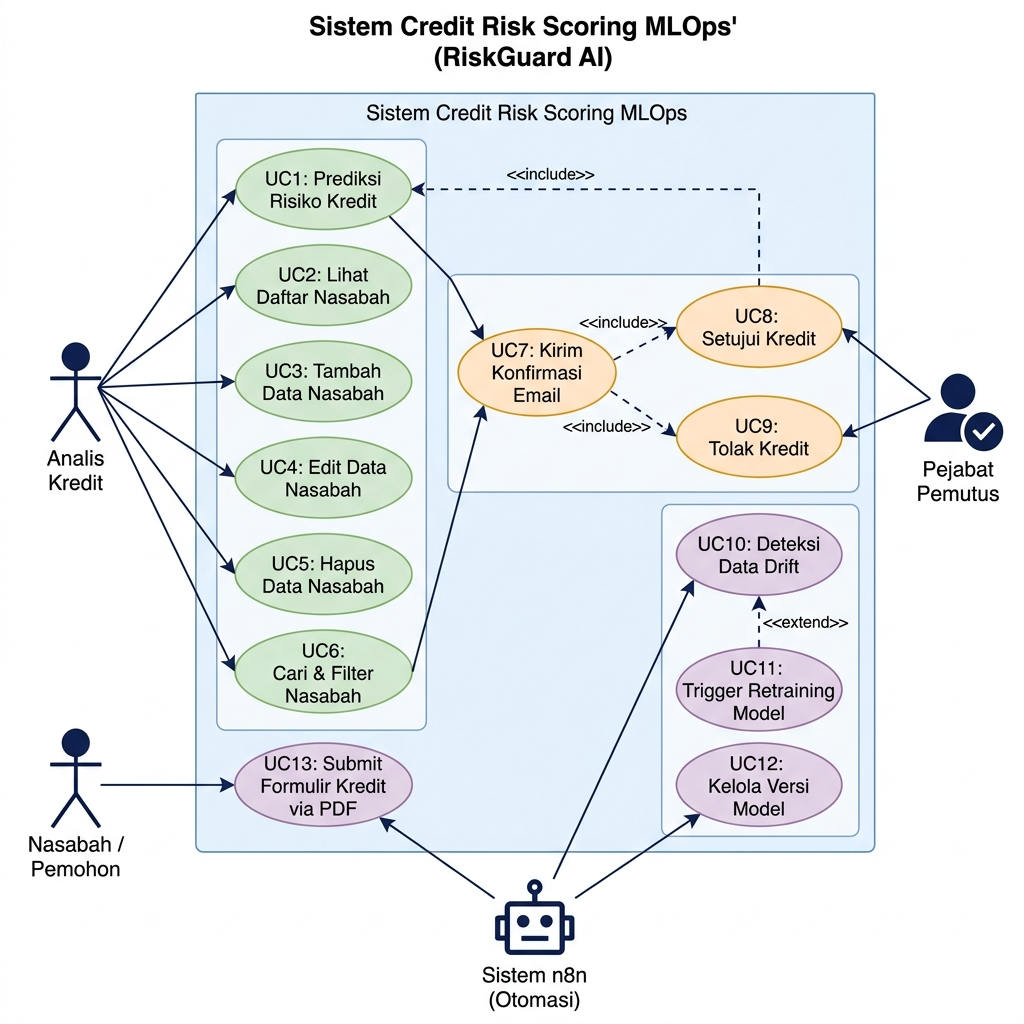
\includegraphics[width=0.92\textwidth]{bab4/use_case_diagram_1783675834026.png}
\caption{Diagram use case keseluruhan sistem credit risk scoring berbasis MLOps}
\label{fig:bab4_use_case_diagram}
\end{figure}

\section{Validasi Awal Dataset Sintetis}
\label{sec:bab4_dataset_sintetis}
Bagian ini menyajikan hasil validasi awal terhadap dataset sintetis yang rancangan pembentukannya telah dijelaskan pada Bab III. Validasi dilakukan untuk memastikan bahwa struktur atribut, format nilai, dan relasi antarkolom pada sampel data tetap konsisten dengan karakteristik umum data kredit konsumtif pada praktik perbankan.

Sebanyak 50 baris sampel data sintetis ditinjau sebagai bagian dari pemeriksaan kewajaran struktur data. Tabel \ref{tab:nasabah_normal} menampilkan 10 baris sampel dari data yang telah ditinjau tersebut. Sampel ini digunakan sebagai bukti bahwa dataset tidak hanya dibangkitkan secara numerik, tetapi juga memiliki atribut identitas, pekerjaan, finansial, histori kredit, parameter risiko, dan indikator makroekonomi yang saling berhubungan secara logis.

\begin{landscape}
\begin{scriptsize}
\setlength{\tabcolsep}{2pt}
\begin{longtable}{p{3.2cm} *{10}{>{\centering\arraybackslash}p{1.1cm}}}
\caption{Profil Data 10 Nasabah Normal}
\label{tab:nasabah_normal} \\
\toprule
\textbf{Fitur / Atribut} & \textbf{Nasabah 1} & \textbf{Nasabah 2} & \textbf{Nasabah 3} & \textbf{Nasabah 4} & \textbf{Nasabah 5} & \textbf{Nasabah 6} & \textbf{Nasabah 7} & \textbf{Nasabah 8} & \textbf{Nasabah 9} & \textbf{Nasabah 10} \\
\midrule
\endfirsthead
\multicolumn{11}{c}{{\tablename\ \thetable{} -- Lanjutan dari halaman sebelumnya}} \\
\toprule
\textbf{Fitur / Atribut} & \textbf{Nasabah 1} & \textbf{Nasabah 2} & \textbf{Nasabah 3} & \textbf{Nasabah 4} & \textbf{Nasabah 5} & \textbf{Nasabah 6} & \textbf{Nasabah 7} & \textbf{Nasabah 8} & \textbf{Nasabah 9} & \textbf{Nasabah 10} \\
\midrule
\endhead
\midrule
\multicolumn{11}{r}{{Bersambung ke halaman berikutnya...}} \\
\endfoot
\bottomrule
\endlastfoot
Customer ID & CUST00001 & CUST00002 & CUST00004 & CUST00007 & CUST00009 & CUST00016 & CUST00019 & CUST00020 & CUST00035 & CUST00036 \\
Nama Nasabah & Gina Pudjiastuti & Violet Utami & Jinawi Prakasa & Padmi Wasita & Ir. Rini Hidayanto & Eman Suartini & Shakila Safitri & Darijan Nababan & Drs. Aurora Pertiwi, S.I.Kom & Wage Najmudin \\
Usia & 64 tahun & 59 tahun & 52 tahun & 63 tahun & 55 tahun & 47 tahun & 46 tahun & 68 tahun & 63 tahun & 56 tahun \\
Jenis Kelamin & Perempuan & Perempuan & Perempuan & Laki-laki & Perempuan & Perempuan & Laki-laki & Perempuan & Perempuan & Laki-laki \\
Status Pernikahan & Menikah & Belum menikah & Menikah & Menikah & Menikah & Cerai & Menikah & Menikah & Cerai & Menikah \\
Jenis Pekerjaan & Pensiunan & Pensiunan & Pensiunan & Pensiunan & Pensiunan & Pensiunan & PNS Purna Bakti & Pensiunan & Pensiunan & Pensiunan \\
Status Pensiun & Pensiun & Pensiun & Pensiun & Pensiun & Aktif & Menjelang pensiun & Menjelang pensiun & Pensiun & Pensiun & Pensiun \\
Pendapatan Bulanan & Rp 3.794.553 & Rp 3.285.278 & Rp 7.896.082 & Rp 837.852 & Rp 2.640.712 & Rp 7.998.989 & Rp 7.068.094 & Rp 6.269.345 & Rp 5.789.716 & Rp 5.299.319 \\
Jumlah Uang Pensiun & Rp 3.035.642 & Rp 2.628.222 & Rp 6.316.866 & Rp 670.282 & Rp 2.112.569 & Rp 6.399.191 & Rp 0 & Rp 5.015.476 & Rp 4.631.773 & Rp 4.239.455 \\
Sumber Gaji & Taspen & Taspen & Kementerian & Kementerian & Taspen & Taspen & Kementerian & Pemerintah Daerah & Kementerian & Kementerian \\
Skor Risiko Pemberi Kerja & 9,72\% & 8,37\% & 9,41\% & 8,70\% & 8,81\% & 11,93\% & 15,67\% & 10,63\% & 10,25\% & 9,35\% \\
Tipe Pemberi Kerja & Government & Government & Swasta & Government & Government & Government & BUMN & BUMN & Government & Government \\
Stabilitas Pendapatan & 50,00\% & 78,17\% & 98,09\% & 95,88\% & 100,00\% & 95,49\% & 70,55\% & 81,02\% & 69,52\% & 64,78\% \\
Rasio Pengeluaran Medis & 42,09\% & 36,60\% & 25,91\% & 40,74\% & 24,38\% & 18,96\% & 16,92\% & 45,00\% & 24,10\% & 31,42\% \\
Volatilitas Gaji & 37,10\% & 20,05\% & 16,83\% & 11,53\% & 10,51\% & 13,87\% & 22,64\% & 19,19\% & 33,76\% & 20,44\% \\
Saldo Rekening Rata-rata & Rp 5.694.253 & Rp 3.940.751 & Rp 8.783.769 & Rp 671.276 & Rp 6.221.424 & Rp 8.226.630 & Rp 17.486.307 & Rp 18.058.906 & Rp 8.497.370 & Rp 10.093.795 \\
Total Cicilan Aktif & 4 & 3 & 3 & 1 & 2 & 3 & 2 & 4 & 3 & 3 \\
Jumlah Pinjaman Lain & 0 & 1 & 2 & 1 & 0 & 1 & 2 & 2 & 0 & 2 \\
Debt-to-Income (DTI) & 60,00\% & 60,00\% & 60,00\% & 60,00\% & 60,00\% & 60,00\% & 60,00\% & 60,00\% & 60,00\% & 60,00\% \\
Skor Kredit Biro (OJK) & 760 & 706 & 615 & 733 & 691 & 704 & 782 & 659 & 755 & 686 \\
Bulan Tunggakan (Past Due) & 0 & 0 & 0 & 0 & 1 & 0 & 0 & 0 & 1 & 2 \\
Lama Riwayat Kredit & 7 tahun & 4 tahun & 5 tahun & 13 tahun & 16 tahun & 5 tahun & 14 tahun & 12 tahun & 8 tahun & 11 tahun \\
Skor Risiko Kesehatan & 0,3954 & 0,6984 & 0,3497 & 0,4720 & 0,3358 & 0,3863 & 0,3126 & 0,4848 & 0,4040 & 0,6703 \\
Memiliki Penyakit Kronis & Tidak & Tidak & Tidak & Ya & Tidak & Ya & Tidak & Tidak & Ya & Tidak \\
Grade Pemeriksaan Medis & Kuning & Hijau & Hijau & Kuning & Hijau & Hijau & Hijau & Hijau & Hijau & Merah \\
Status Asuransi Jiwa & Ada & Ada & Ada & Ada & Ada & Ada & Ada & Ada & Ada & Lapsed \\
Uang Pertanggungan Asuransi & Rp 74.568.148 & Rp 93.427.960 & Rp 160.876.644 & Rp 19.522.187 & Rp 60.489.422 & Rp 106.996.685 & Rp 210.987.989 & Rp 77.736.947 & Rp 111.620.706 & Rp 0 \\
Perusahaan Asuransi & A & N/A & N/A & C & N/A & A & B & B & N/A & A \\
Premi Asuransi Bulanan & Rp 41.236 & Rp 37.399 & Rp 322.020 & Rp 19.283 & Rp 90.346 & Rp 309.770 & Rp 127.723 & Rp 234.098 & Rp 68.648 & Rp 0 \\
Loan ID & LOAN00001 & LOAN00002 & LOAN00004 & LOAN00007 & LOAN00009 & LOAN00016 & LOAN00019 & LOAN00020 & LOAN00035 & LOAN00036 \\
Jenis Produk Kredit & Kredit Pensiun & KTA & Vehicle Loan & KTA & Kredit Pensiun & Vehicle Loan & KTA & Vehicle Loan & Payroll loan & Kredit Pensiun \\
Tanggal Pencairan & 2024-07-07 & 2024-08-29 & 2024-10-19 & 2024-12-25 & 2024-05-18 & 2024-07-12 & 2024-06-29 & 2024-10-24 & 2024-07-02 & 2024-04-19 \\
Jumlah Pinjaman & Rp 445.817.427 & Rp 91.001.085 & Rp 259.288.337 & Rp 133.424.947 & Rp 229.291.603 & Rp 378.063.313 & Rp 352.642.843 & Rp 81.310.033 & Rp 281.474.657 & Rp 393.324.410 \\
Tenor (Bulan) & 36 bulan & 24 bulan & 36 bulan & 24 bulan & 60 bulan & 60 bulan & 36 bulan & 12 bulan & 36 bulan & 60 bulan \\
Suku Bunga & 10,26\% & 7,05\% & 7,29\% & 6,19\% & 7,67\% & 11,50\% & 6,81\% & 8,74\% & 6,22\% & 11,79\% \\
Memiliki Agunan & Tidak & Tidak & Ya & Tidak & Tidak & Ya & Tidak & Ya & Tidak & Tidak \\
Loan-to-Value (LTV) & 0,00\% & 0,00\% & 73,78\% & 0,00\% & 0,00\% & 64,68\% & 0,00\% & 81,00\% & 0,00\% & 0,00\% \\
Sisa Pinjaman (Outstanding) & Rp 339.481.396 & Rp 51.108.601 & Rp 210.129.567 & Rp 80.717.080 & Rp 211.496.051 & Rp 311.998.546 & Rp 217.816.877 & Rp 40.116.401 & Rp 257.162.920 & Rp 224.891.067 \\
Penarikan Tunai Terakhir & Rp 1.689.874 & Rp 1.593.090 & Rp 2.431.573 & Rp 107.371 & Rp 329.034 & Rp 3.057.805 & Rp 1.558.622 & Rp 1.474.772 & Rp 619.314 & Rp 2.179.738 \\
Frekuensi Transaksi Digital & 6 & 4 & 2 & 5 & 4 & 8 & 6 & 6 & 6 & 2 \\
Pengeluaran Kartu & Rp 2.344.281 & Rp 1.305.067 & Rp 5.289.440 & Rp 516.051 & Rp 653.734 & Rp 4.066.357 & Rp 3.243.903 & Rp 4.285.389 & Rp 3.809.882 & Rp 2.027.416 \\
Probability of Default (PD) & 17,80\% & 33,58\% & 44,18\% & 22,13\% & 49,17\% & 60,25\% & 12,13\% & 41,57\% & 72,54\% & 95,22\% \\
Flag Gagal Bayar & 0 (Normal) & 0 (Normal) & 0 (Normal) & 0 (Normal) & 0 (Normal) & 0 (Normal) & 0 (Normal) & 0 (Normal) & 0 (Normal) & 0 (Normal) \\
Loss Given Default (LGD) & 35,53\% & 40,37\% & 26,14\% & 43,17\% & 41,50\% & 25,31\% & 37,87\% & 28,95\% & 31,98\% & 54,85\% \\
Exposure at Default (EAD) & Rp 335.521.586 & Rp 46.974.181 & Rp 206.268.544 & Rp 78.150.696 & Rp 193.322.196 & Rp 282.194.173 & Rp 211.283.836 & Rp 38.057.267 & Rp 236.291.708 & Rp 209.726.895 \\
Expected Loss (EL) & Rp 21.228.120 & Rp 6.368.037 & Rp 23.822.213 & Rp 7.467.822 & Rp 39.453.423 & Rp 43.035.391 & Rp 9.705.088 & Rp 4.579.550 & Rp 54.818.226 & Rp 109.536.605 \\

\end{longtable}
\end{scriptsize}
\end{landscape}

Berdasarkan sampel tersebut, dataset sintetis dinilai memadai untuk digunakan pada tahap pengujian berikutnya karena telah memuat variasi atribut nasabah, produk kredit, indikator risiko, serta variabel makroekonomi yang dibutuhkan dalam proses \textit{credit risk scoring}. Dengan demikian, pengujian pada bagian selanjutnya dapat difokuskan pada kualitas preprocessing, performa model, validasi quality gate, dan kesiapan implementasi MLOps.


\section{Pengujian Preprocessing WoE dan IV}
\label{sec:bab4_preprocessing_woe_iv}
Tahap preprocessing menggunakan \textit{Weight of Evidence} (WoE) untuk mengubah fitur numerik dan kategorikal menjadi representasi yang berkaitan dengan \textit{log-odds} gagal bayar. Sementara itu, \textit{Information Value} (IV) digunakan untuk menilai kekuatan prediktif setiap fitur terhadap target \textit{missed\_payment\_flag}. Kombinasi WoE dan IV dipilih karena umum digunakan pada \textit{credit scoring}, mudah dijelaskan, dan dapat membantu membedakan fitur yang informatif dari fitur yang bersifat noise.

Hasil perhitungan IV menunjukkan bahwa fitur \textit{bureau\_score} menjadi prediktor terkuat dengan nilai IV sebesar 0,408071. Fitur ini dikategorikan sebagai \textit{strong predictor}, sehingga dipertahankan sebagai masukan penting bagi model. Beberapa fitur lain seperti \textit{past\_due\_months}, \textit{marital\_status}, \textit{term\_months}, \textit{age}, \textit{life\_insurance\_coverage}, \textit{insurance\_premium\_monthly}, dan \textit{insurance\_status} berada pada kategori \textit{medium predictor}. Fitur dengan nilai IV di bawah 0,02, seperti \textit{credit\_history\_length}, \textit{avg\_account\_balance}, \textit{digital\_payment\_frequency}, dan beberapa fitur makroekonomi, dieliminasi karena kontribusi prediktifnya sangat rendah.

\begin{table}[H]
\centering
\caption{Ringkasan fitur utama berdasarkan nilai Information Value}
\label{tab:bab4_iv_summary}
\begin{tabular}{|p{0.06\textwidth}|p{0.32\textwidth}|p{0.17\textwidth}|p{0.27\textwidth}|}
\hline
\textbf{No.} & \textbf{Fitur} & \textbf{Nilai IV} & \textbf{Interpretasi} \\
\hline
1 & \textit{bureau\_score} & 0,408071 & \textit{Strong predictor} \\
\hline
2 & \textit{past\_due\_months} & 0,215358 & \textit{Medium predictor} \\
\hline
3 & \textit{marital\_status} & 0,164296 & \textit{Medium predictor} \\
\hline
4 & \textit{term\_months} & 0,154057 & \textit{Medium predictor} \\
\hline
6 & \textit{life\_insurance\_coverage} & 0,112946 & \textit{Medium predictor} \\
\hline
7 & \textit{insurance\_premium\_monthly} & 0,112611 & \textit{Medium predictor} \\
\hline
8 & \textit{insurance\_status} & 0,105535 & \textit{Medium predictor} \\
\hline
\end{tabular}
\end{table}

\begin{figure}[H]
\centering
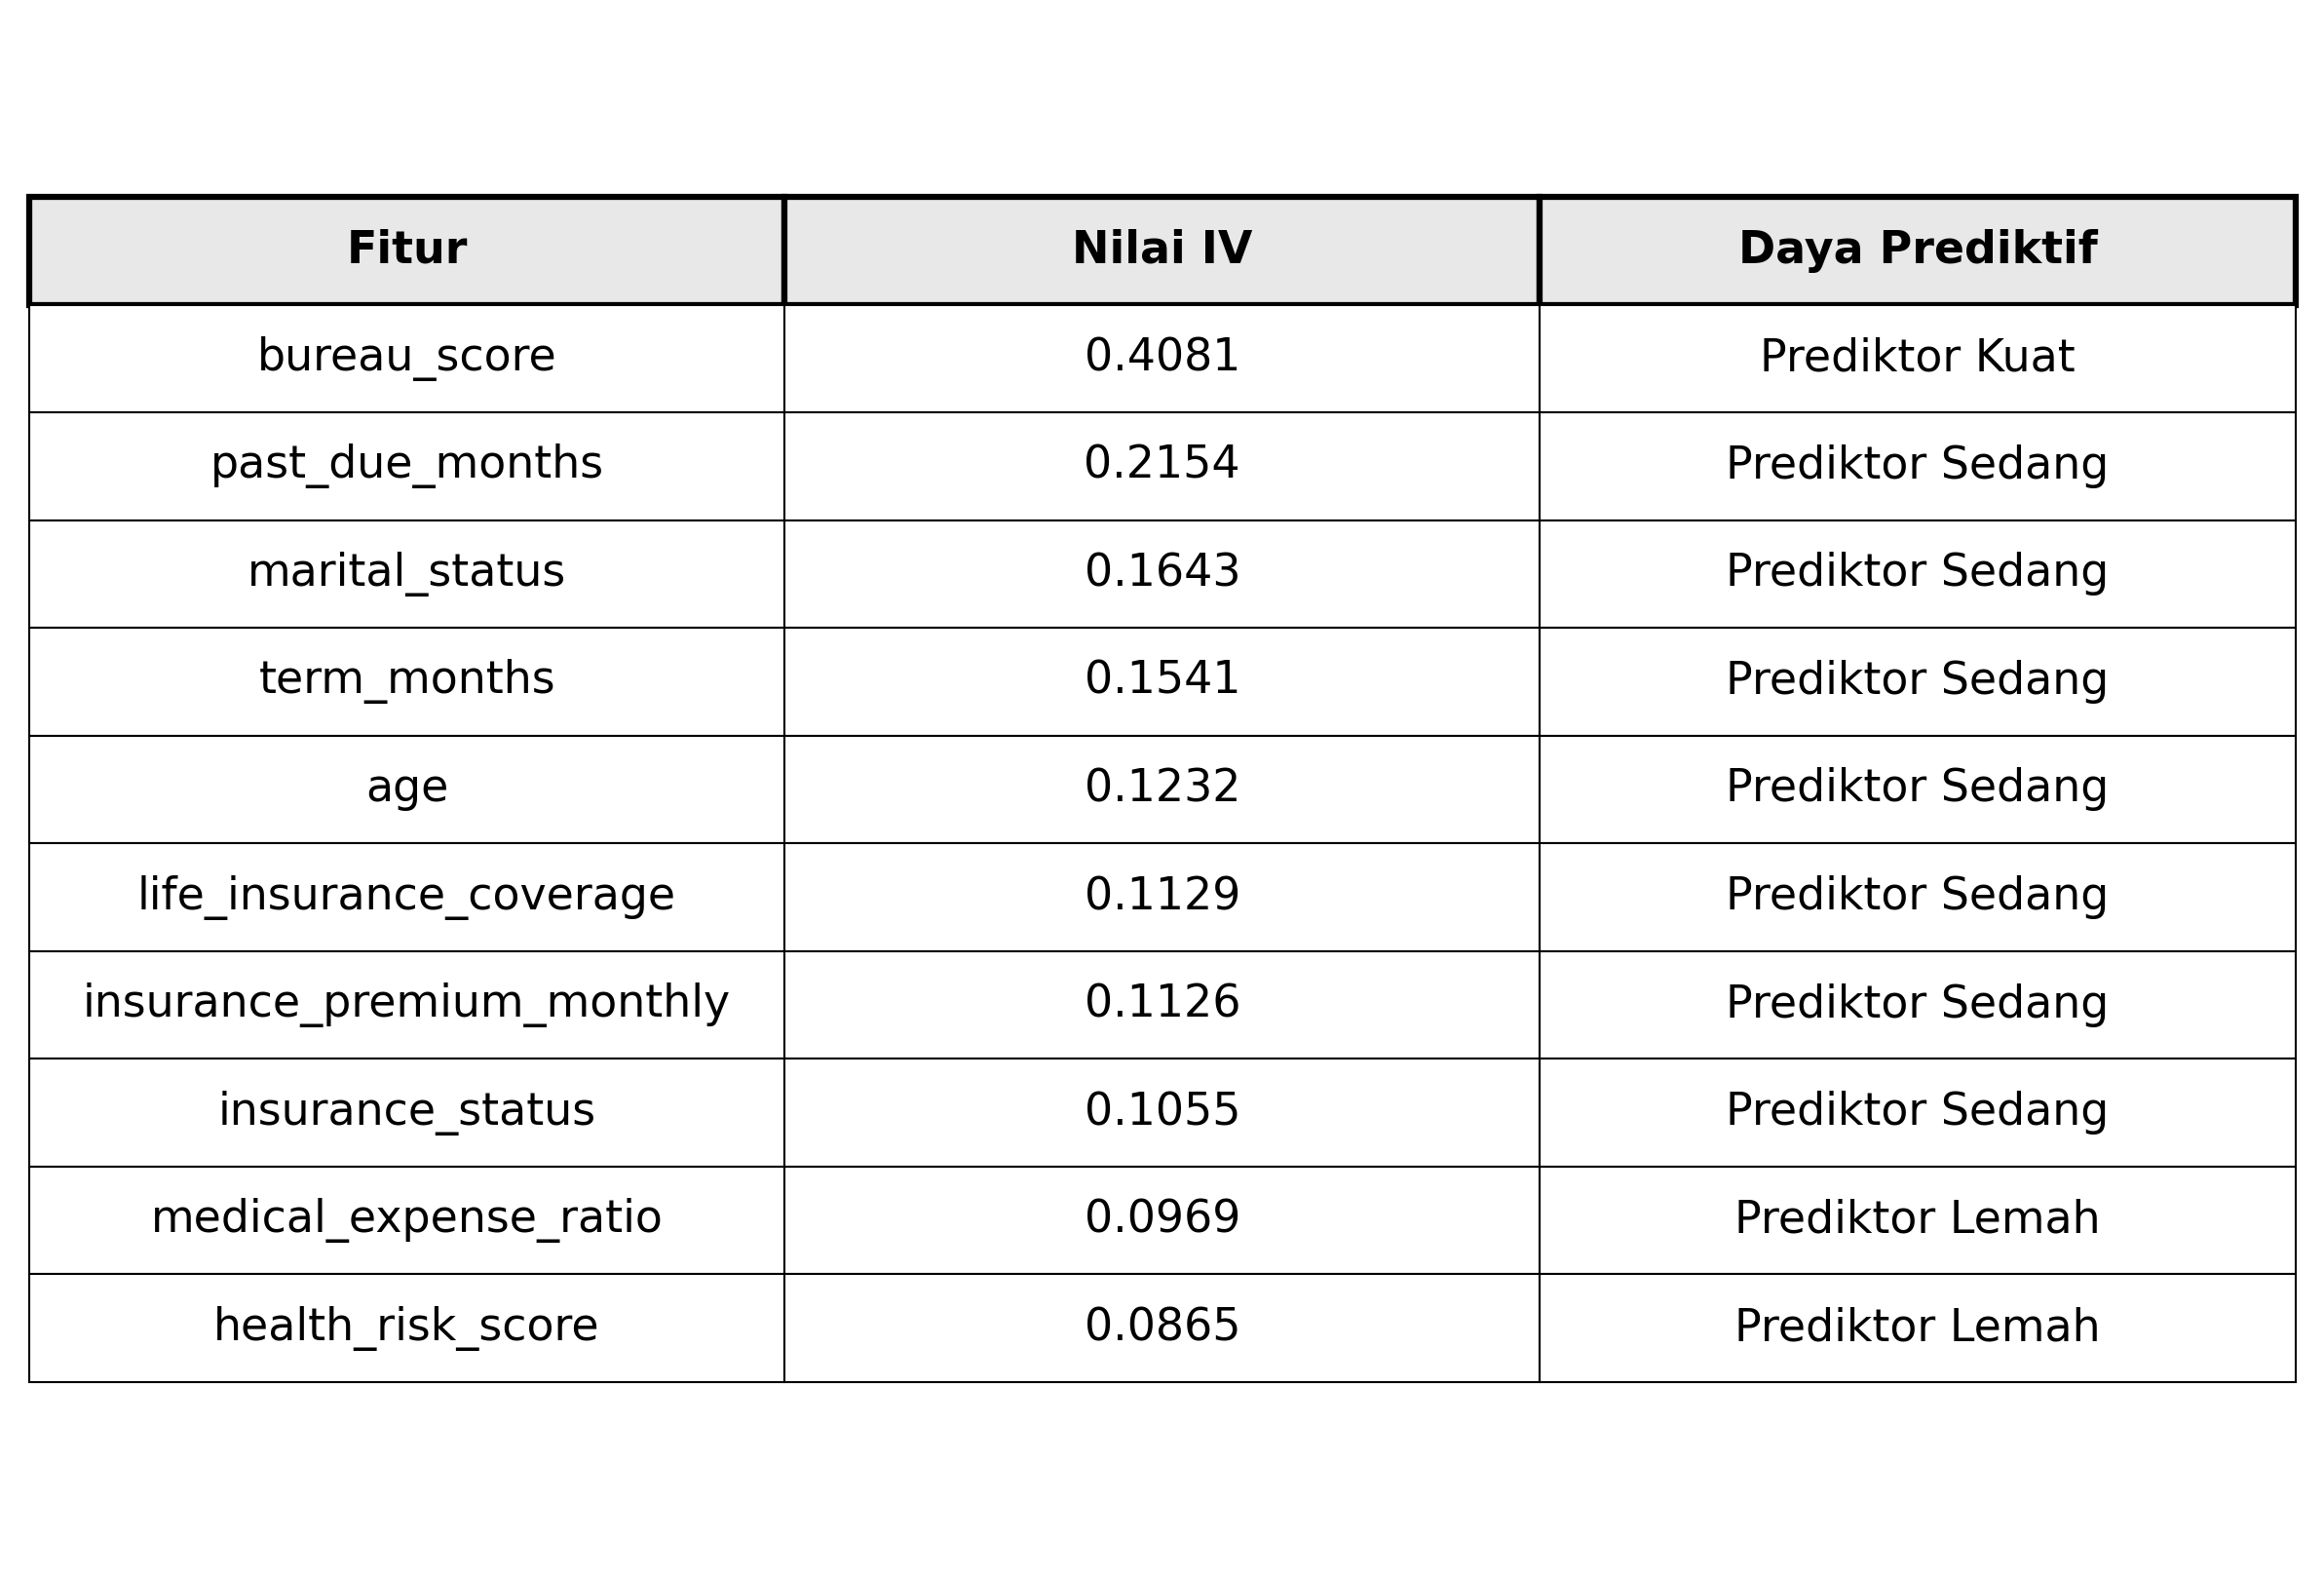
\includegraphics[width=0.9\textwidth]{bab4/Tabel_IV_Format.png}
\caption{Tabel nilai Information Value untuk seleksi fitur}
\label{fig:bab4_tabel_iv}
\end{figure}



Selain nilai IV, hasil binning WoE digunakan untuk melihat pola hubungan antara kelompok nilai fitur dan risiko gagal bayar. Gambar \ref{fig:bab4_woe_binning} menunjukkan bahwa setiap bin memiliki nilai WoE yang dapat dibandingkan, sehingga perubahan tingkat risiko pada masing-masing kelompok fitur dapat dianalisis secara lebih terstruktur.

\begin{figure}[H]
\centering
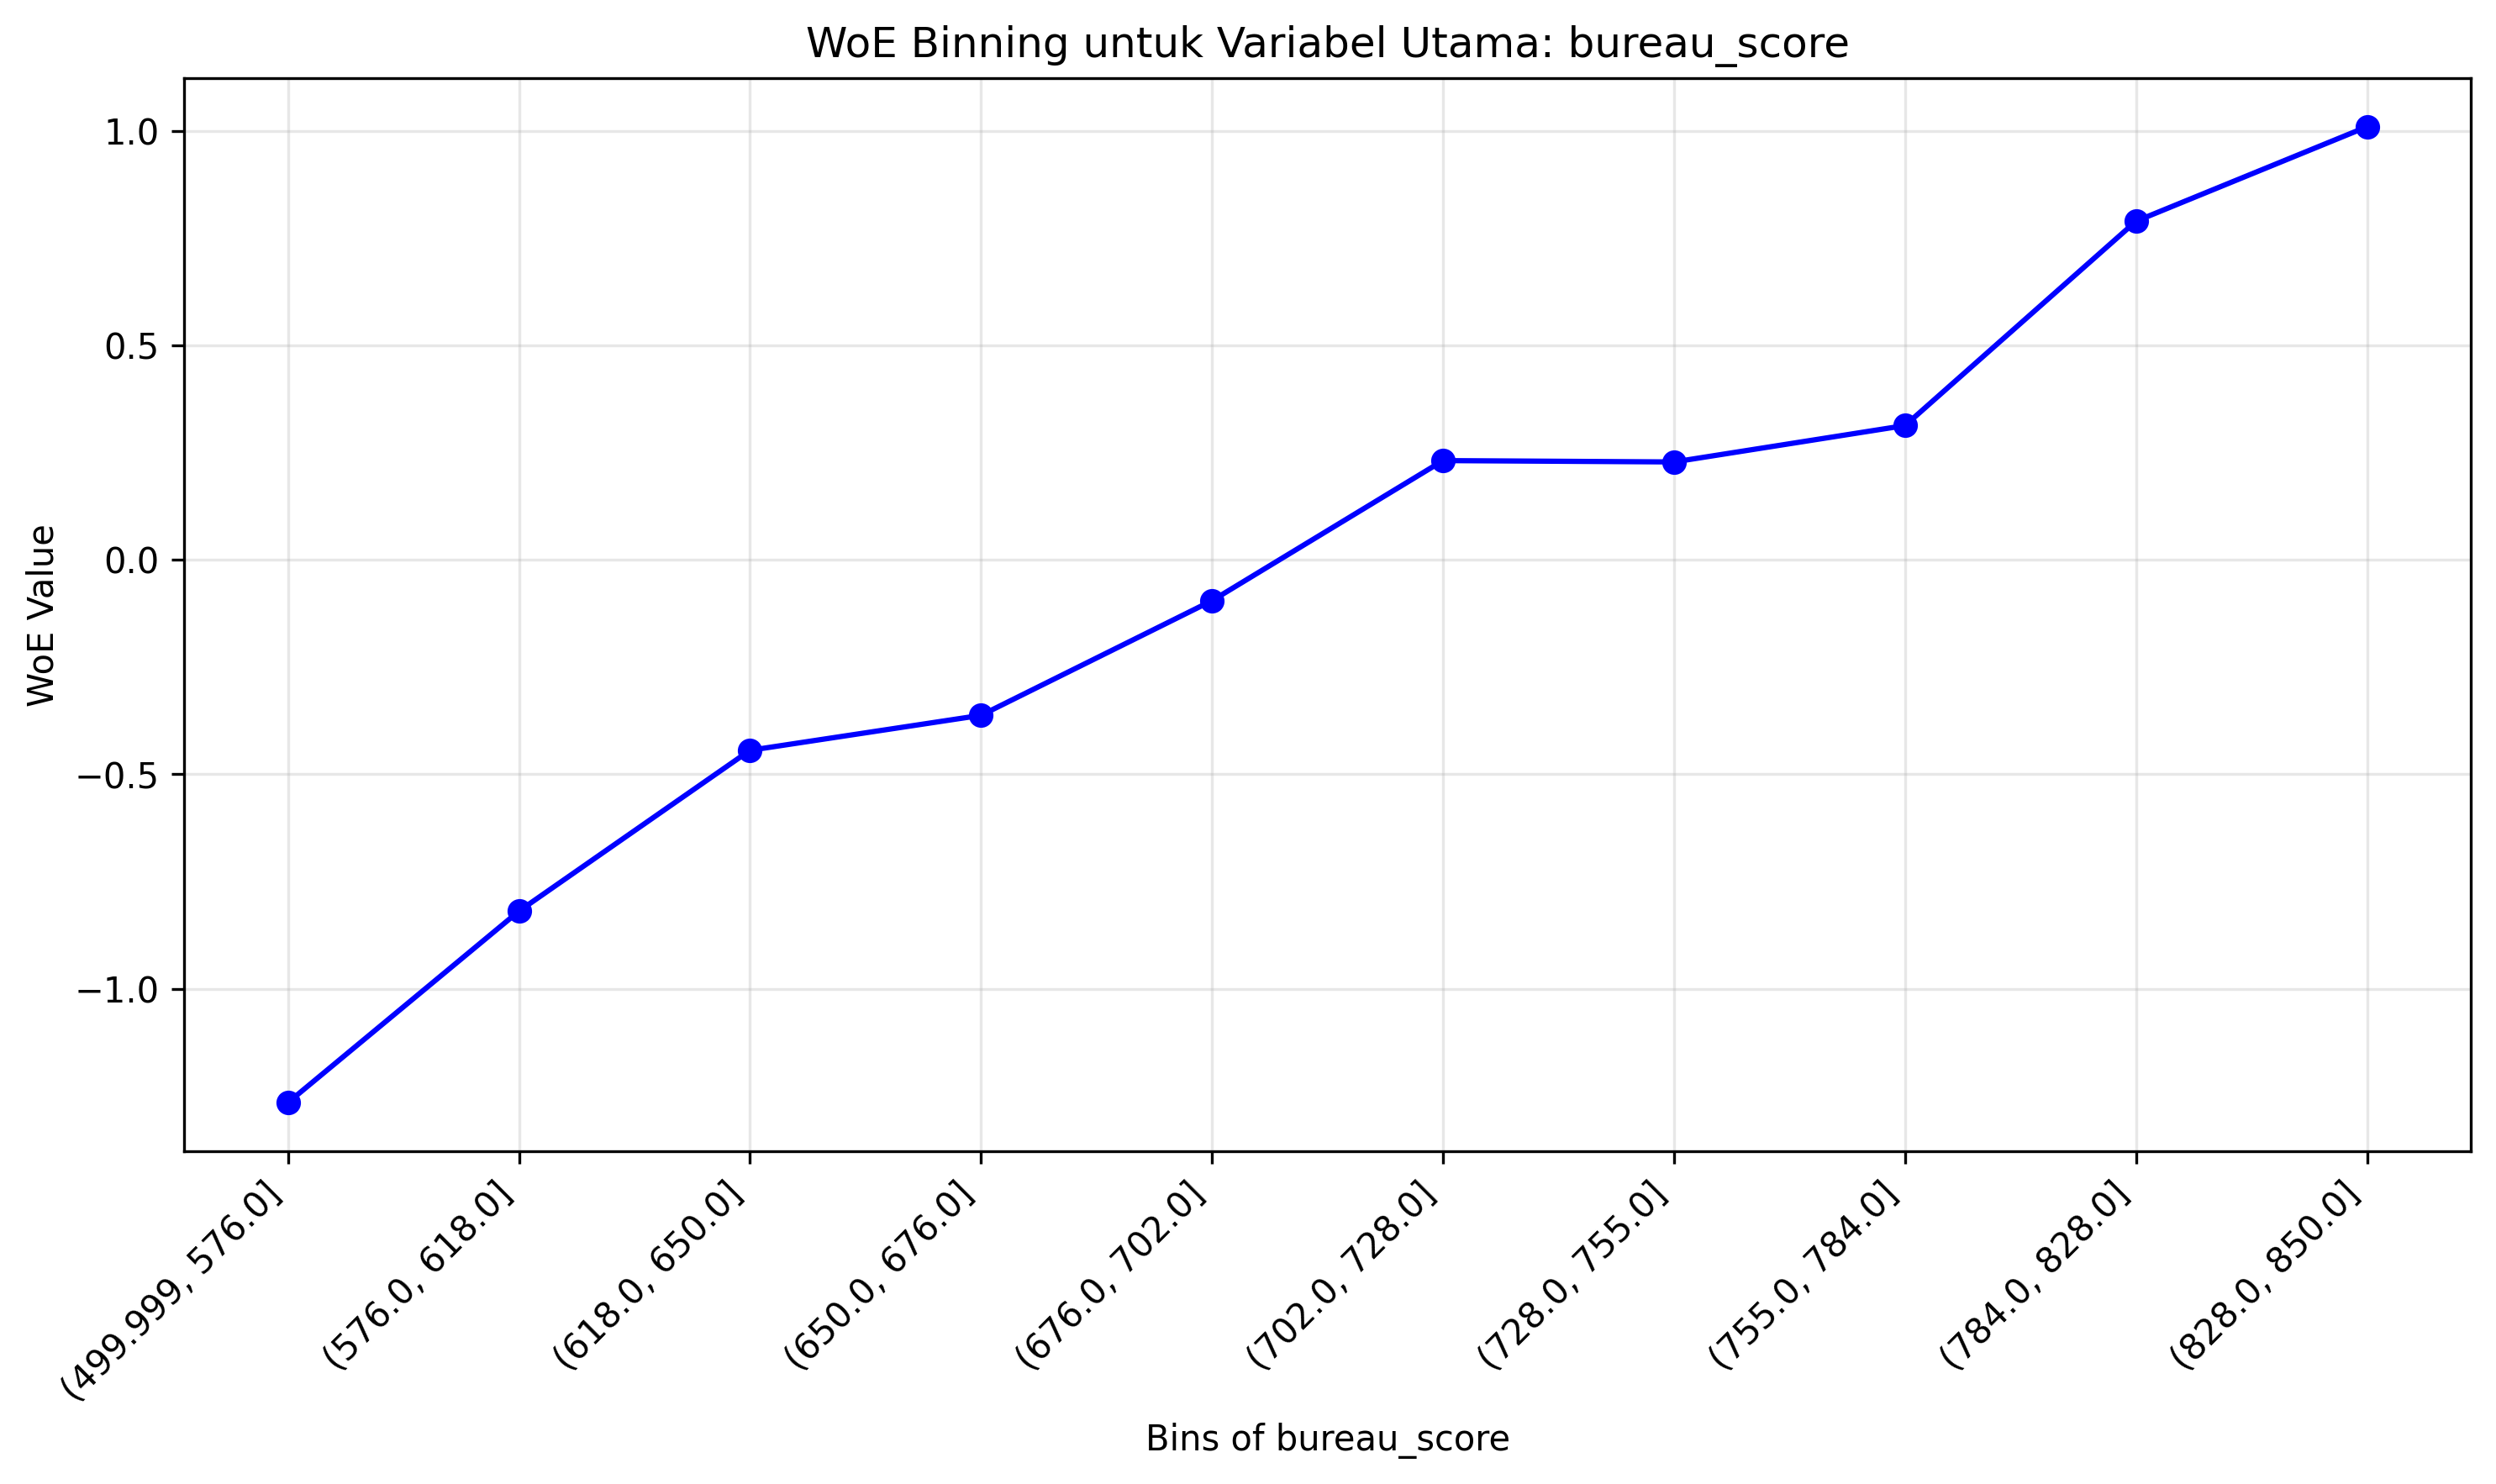
\includegraphics[width=0.86\textwidth]{bab4/WoE_Binning_plot.png}
\caption{Visualisasi WoE binning pada fitur utama}
\label{fig:bab4_woe_binning}
\end{figure}

\section{Pengujian Penanganan Ketidakseimbangan Kelas}
\label{sec:bab4_smote}
Dataset risiko kredit memiliki karakteristik kelas yang tidak seimbang karena jumlah nasabah yang tidak mengalami gagal bayar lebih besar dibandingkan jumlah nasabah yang mengalami gagal bayar. Pada data awal, kelas non-default berjumlah 8.520 nasabah atau 85,2\%, sedangkan kelas default berjumlah 1.480 nasabah atau 14,8\%. Ketimpangan ini berpotensi membuat model cenderung memprediksi kelas mayoritas dan mengabaikan pola pada kelas default.

Untuk mengatasi masalah tersebut, SMOTE diterapkan pada data latih setelah proses pembagian dataset. Penerapan SMOTE hanya dilakukan pada data latih agar tidak terjadi kebocoran informasi ke data validasi maupun data uji. Hasilnya, jumlah data default pada data latih meningkat sehingga distribusi kelas menjadi seimbang.

\begin{table}[H]
\centering
\caption{Distribusi kelas sebelum dan sesudah SMOTE pada data latih}
\label{tab:bab4_smote}
\begin{tabular}{|p{0.25\textwidth}|p{0.18\textwidth}|p{0.18\textwidth}|p{0.17\textwidth}|p{0.14\textwidth}|}
\hline
\textbf{Kondisi} & \textbf{Non-Default} & \textbf{Default} & \textbf{Total} & \textbf{Rasio} \\
\hline
Sebelum SMOTE & 5.964 & 1.036 & 7.000 & 85,2\% : 14,8\% \\
\hline
Setelah SMOTE & 5.964 & 5.964 & 11.928 & 50,0\% : 50,0\% \\
\hline
\end{tabular}
\end{table}

Hasil ini menunjukkan bahwa proses resampling berhasil menyeimbangkan distribusi kelas pada data latih. Dengan distribusi yang lebih seimbang, proses pembelajaran XGBoost memperoleh sinyal yang lebih proporsional dari kedua kelas, khususnya kelas default yang menjadi fokus utama dalam konteks manajemen risiko kredit.

\section{Pengembangan dan Evaluasi Model}
\label{sec:bab4_pemodelan}
Model utama yang digunakan dalam penelitian ini adalah XGBoost. Pemilihan XGBoost didasarkan pada kemampuannya dalam menangani data tabular, memodelkan interaksi antarfitur secara nonlinier, serta menyediakan mekanisme pengendalian kompleksitas model. Pada tahap pelatihan, data hasil transformasi WoE digunakan sebagai masukan model, sedangkan konfigurasi model dipilih melalui \textit{RandomizedSearchCV} dengan 10 iterasi dan 3-Fold Cross Validation.

Parameter yang diuji meliputi \textit{max\_depth}, \textit{learning\_rate}, \textit{n\_estimators}, \textit{subsample}, dan \textit{colsample\_bytree}. Hasil tuning menunjukkan bahwa konfigurasi terbaik diperoleh pada kedalaman pohon 5, \textit{learning rate} 0,01, jumlah estimator 100, \textit{subsample} 0,8, dan \textit{colsample} 0,8, dengan rata-rata AUC validasi sebesar 0,819303.

\begin{table}[H]
\centering
\caption{Ringkasan hasil hyperparameter tuning XGBoost}
\label{tab:bab4_tuning_summary}
\begin{tabular}{|p{0.12\textwidth}|p{0.14\textwidth}|p{0.16\textwidth}|p{0.16\textwidth}|p{0.14\textwidth}|p{0.16\textwidth}|}
\hline
\textbf{Peringkat} & \textbf{Max Depth} & \textbf{Learning Rate} & \textbf{N Estimators} & \textbf{Subsample} & \textbf{Mean AUC} \\
\hline
1 & 5 & 0,01 & 100 & 0,8 & 0,819303 \\
\hline
2 & 5 & 0,05 & 200 & 0,8 & 0,818365 \\
\hline
3 & 5 & 0,10 & 100 & 0,8 & 0,815952 \\
\hline
4 & 3 & 0,10 & 200 & 0,8 & 0,808289 \\
\hline
5 & 3 & 0,01 & 100 & 0,8 & 0,799574 \\
\hline
\end{tabular}
\end{table}

Visualisasi konfigurasi tuning terbaik ditampilkan pada Gambar \ref{fig:bab4_tabel_tuning}. Dokumentasi parameter ini penting agar proses pelatihan model dapat ditelusuri kembali dan direplikasi.

\begin{figure}[H]
\centering
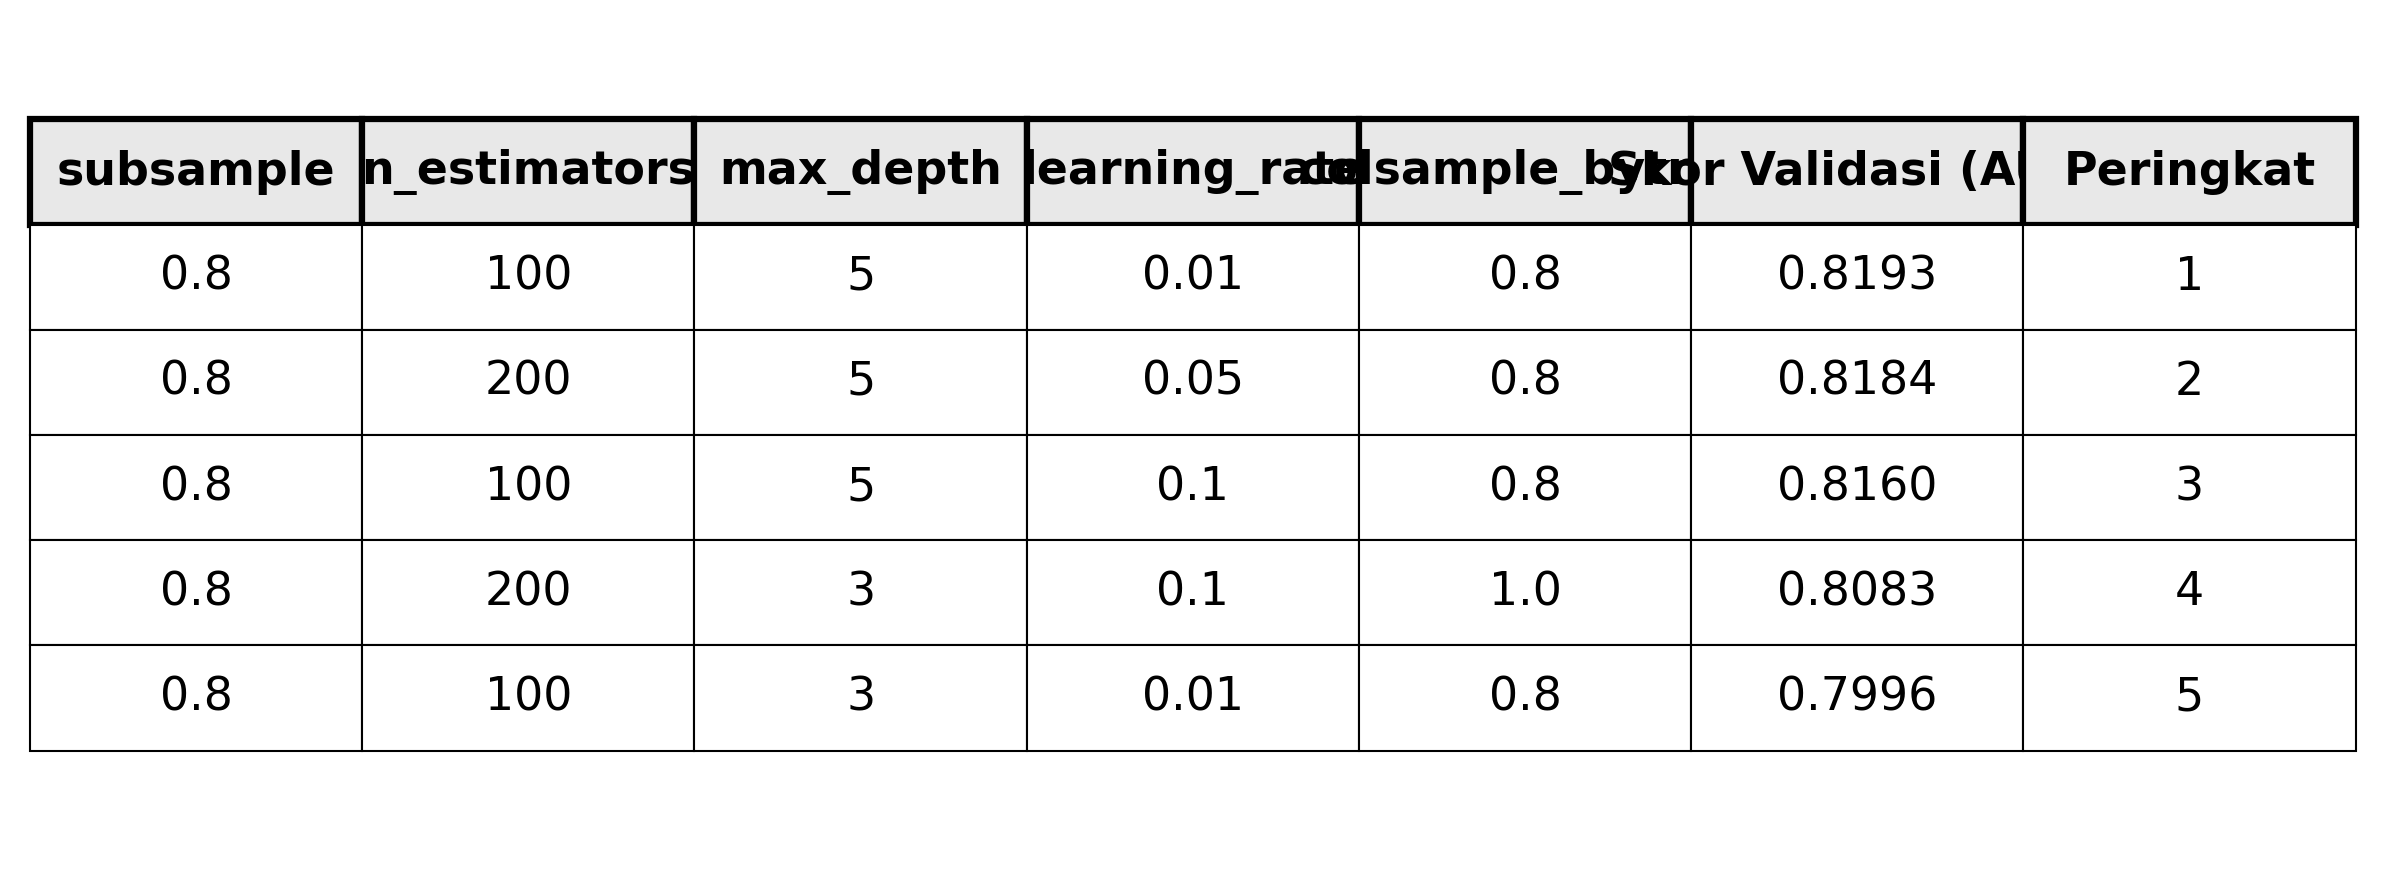
\includegraphics[width=0.86\textwidth]{bab4/Tabel_Tuning_Format.png}
\caption{Konfigurasi hyperparameter terbaik pada model XGBoost}
\label{fig:bab4_tabel_tuning}
\end{figure}

Model terbaik kemudian dievaluasi pada data uji independen. Hasil evaluasi menunjukkan AUC sebesar 0,8262, presisi sebesar 0,8024, recall sebesar 0,7549, dan F1-score sebesar 0,7779. Nilai AUC yang berada di atas 0,80 menunjukkan bahwa model memiliki kemampuan diskriminasi yang baik dalam membedakan nasabah berisiko rendah dan nasabah berisiko tinggi.

Selain metrik evaluasi akhir, proses pelatihan dan pencatatan eksperimen juga diverifikasi melalui antarmuka MLflow. Gambar \ref{fig:bab4_mlflow_experiments} menunjukkan daftar eksperimen \textit{Credit Risk MLOPS} yang tersimpan pada MLflow. Setiap eksperimen merepresentasikan proses pelatihan yang dicatat beserta waktu pembuatan dan pembaruannya, sehingga riwayat eksperimen dapat ditelusuri kembali ketika model perlu dibandingkan atau direproduksi.

\begin{figure}[H]
\centering
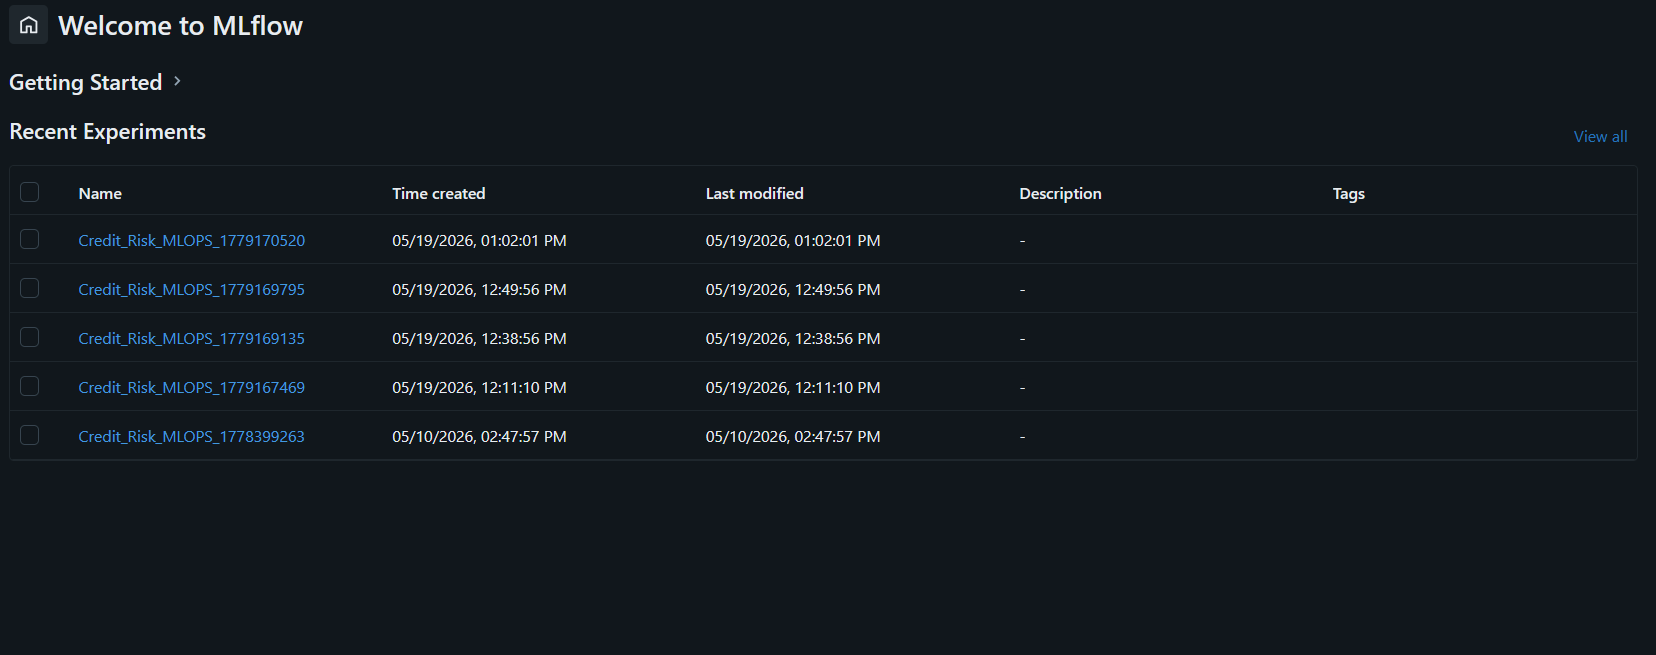
\includegraphics[width=0.92\textwidth]{bab4/Screenshot 2026-05-25 190337.png}
\caption{Daftar eksperimen pelatihan model pada antarmuka MLflow}
\label{fig:bab4_mlflow_experiments}
\end{figure}

\begin{table}[H]
\centering
\caption{Metrik evaluasi model XGBoost pada data uji}
\label{tab:bab4_metrik_model}
\begin{tabular}{|l|c|p{0.45\textwidth}|}
\hline
\textbf{Metrik} & \textbf{Nilai} & \textbf{Interpretasi} \\
\hline
AUC & 0,8262 & Kemampuan diskriminasi model tergolong baik. \\
\hline
Precision & 0,8024 & Sebagian besar prediksi berisiko benar-benar relevan. \\
\hline
Recall & 0,7549 & Model mampu menangkap sebagian besar kasus default. \\
\hline
F1-score & 0,7779 & Keseimbangan presisi dan recall cukup baik. \\
\hline
\end{tabular}
\end{table}

Ringkasan metrik evaluasi juga disajikan pada Gambar \ref{fig:bab4_tabel_metrik}, sedangkan kurva ROC ditunjukkan pada Gambar \ref{fig:bab4_roc_curve}. Kurva ROC digunakan untuk melihat performa model pada berbagai ambang keputusan, bukan hanya pada satu nilai ambang tertentu.

\begin{figure}[H]
\centering
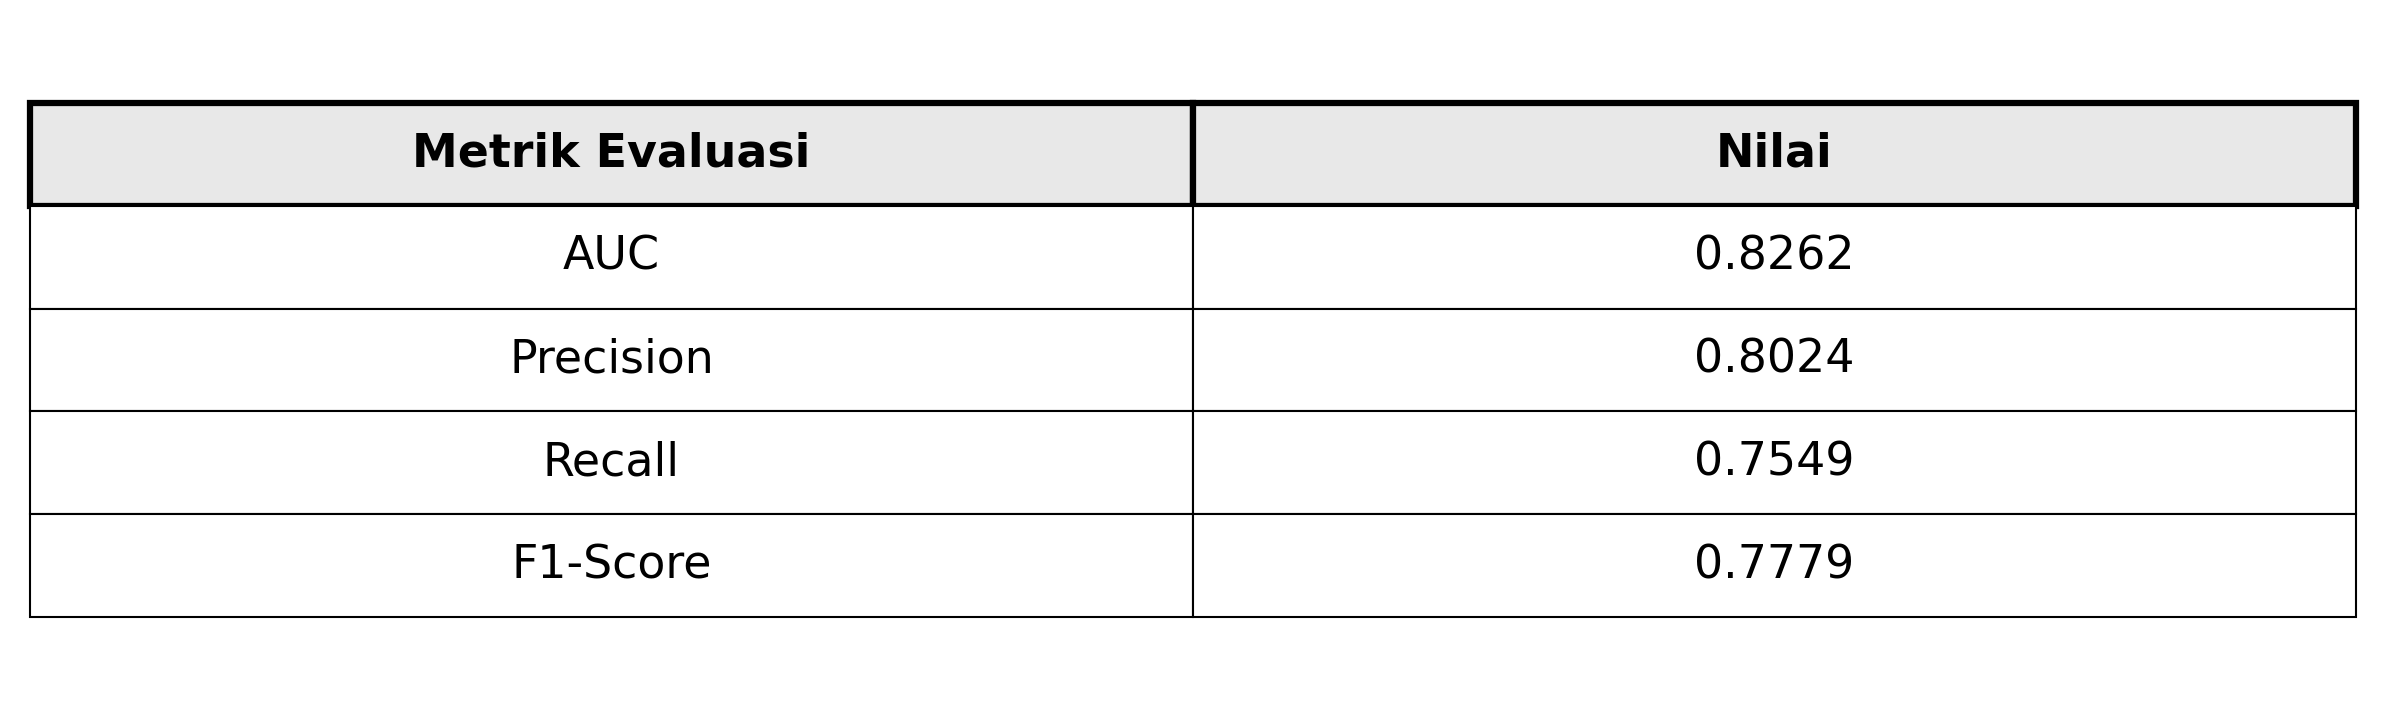
\includegraphics[width=0.86\textwidth]{bab4/Tabel_Metrik_Evaluasi_Format.png}
\caption{Tabel metrik evaluasi model prediktif risiko kredit}
\label{fig:bab4_tabel_metrik}
\end{figure}

\begin{figure}[H]
\centering
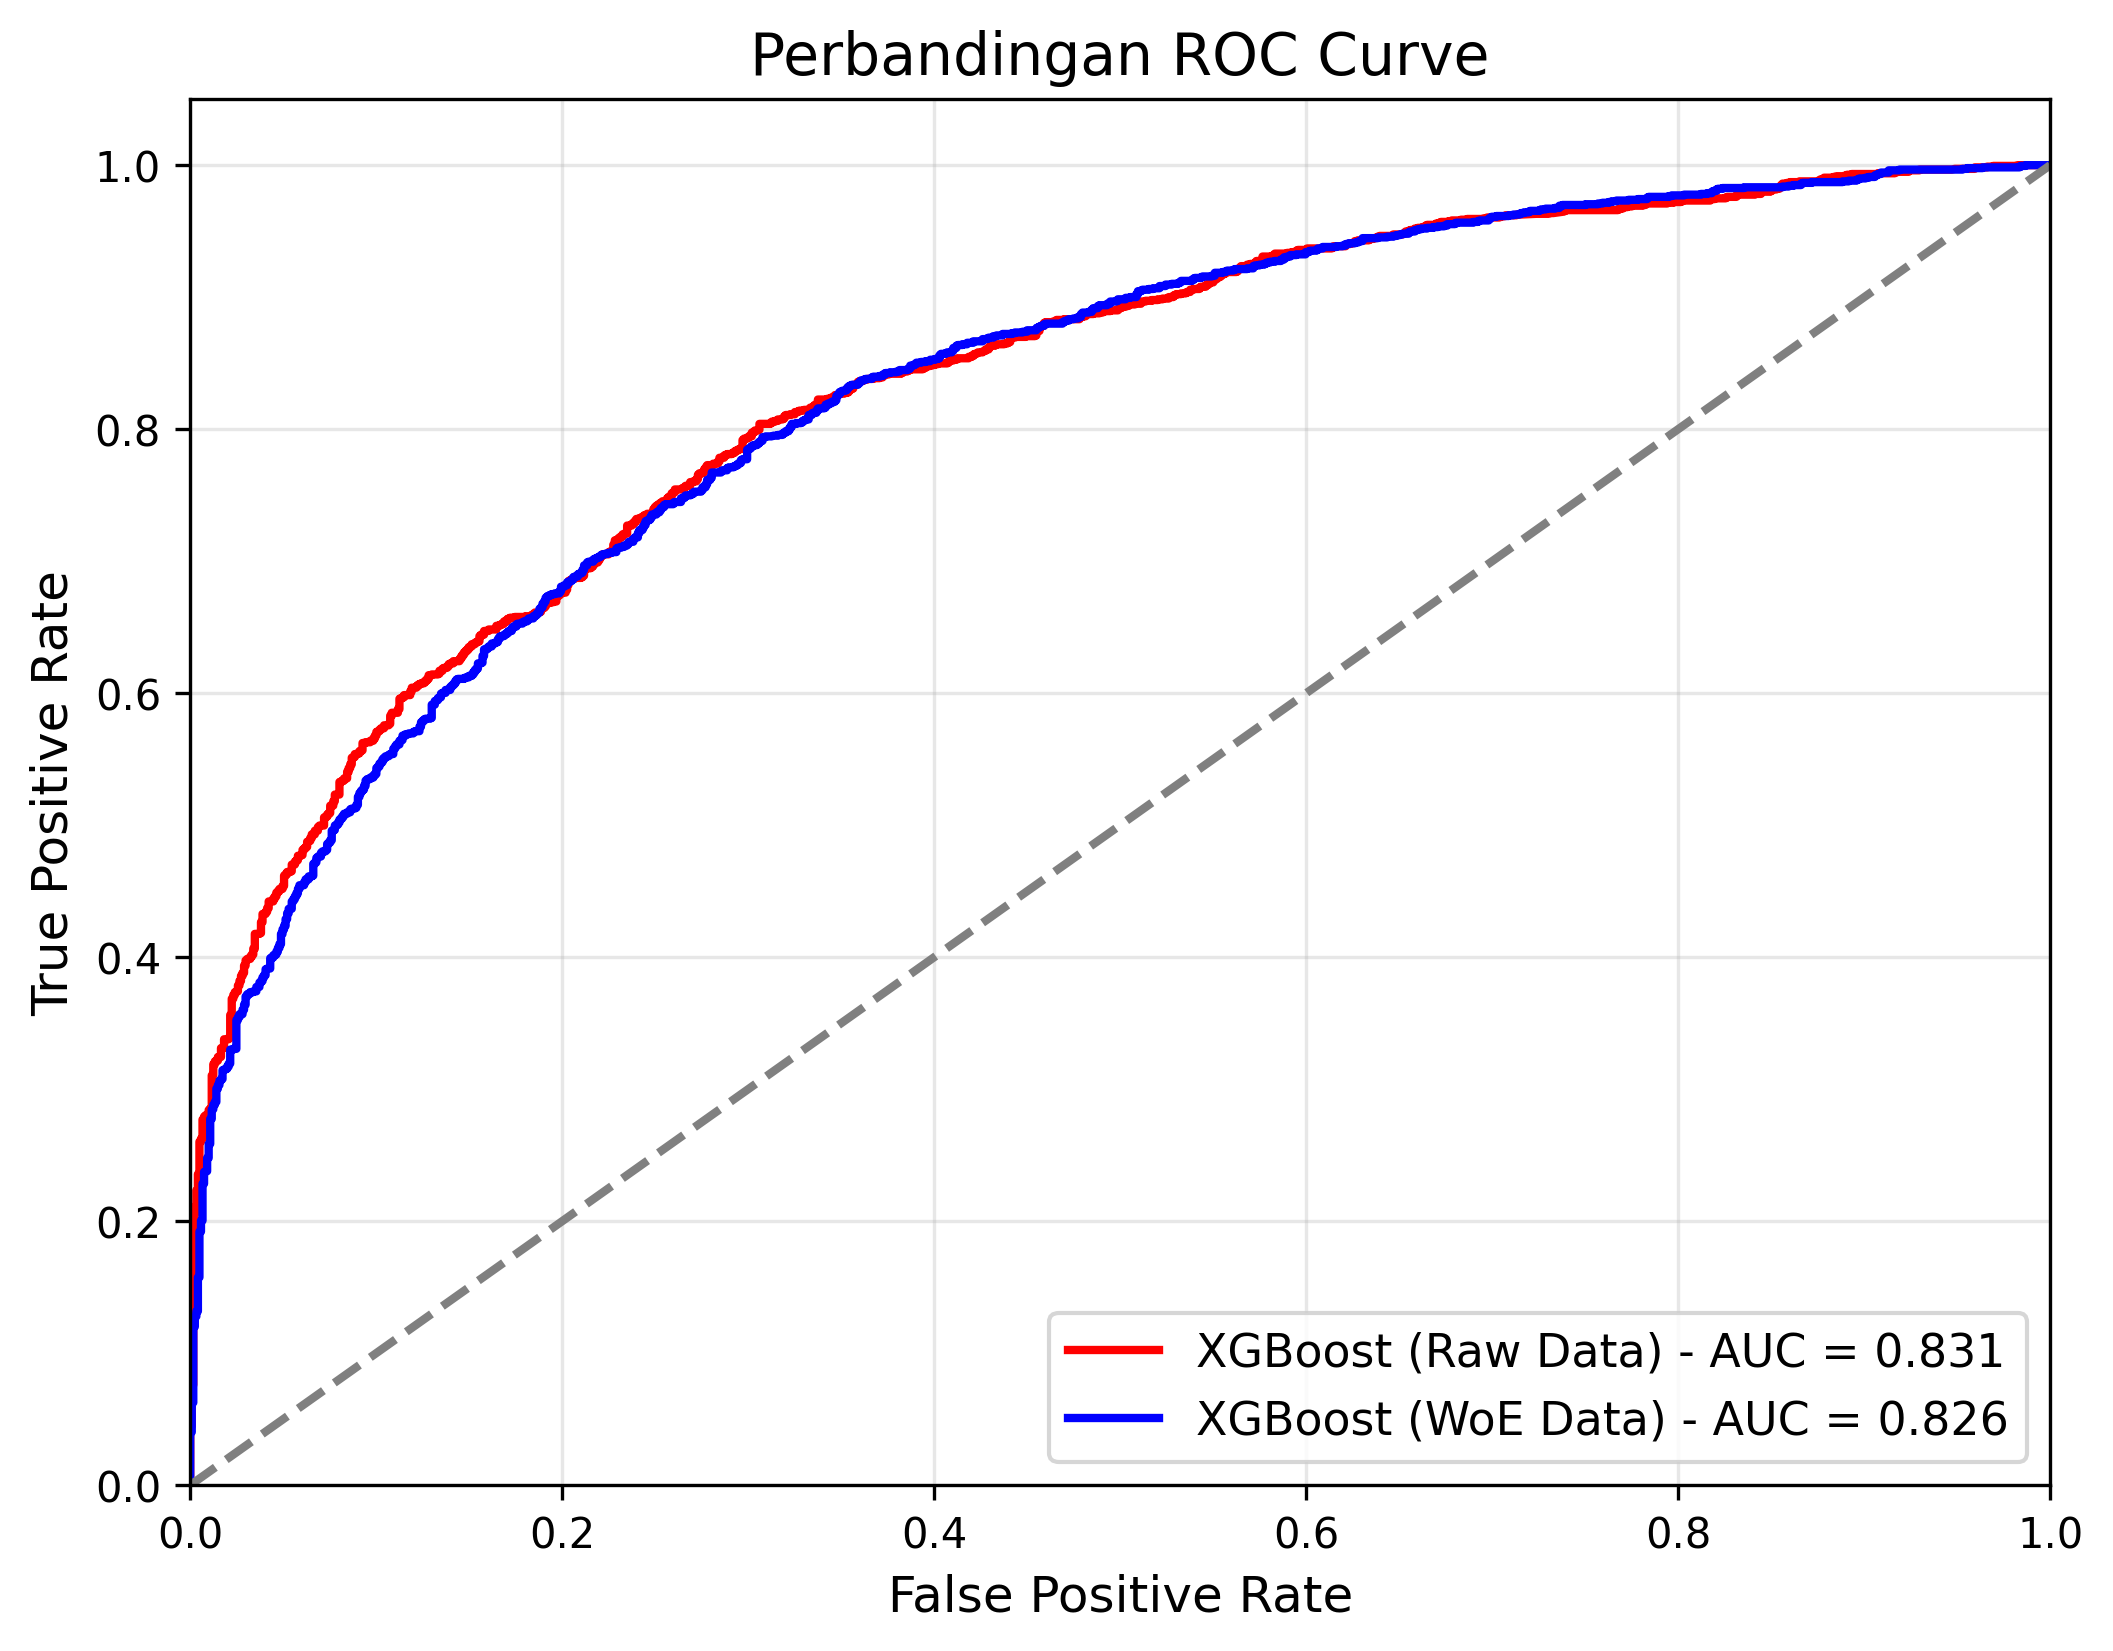
\includegraphics[width=0.8\textwidth]{bab4/ROC_Curve.png}
\caption{Kurva ROC model XGBoost terbaik pada data uji}
\label{fig:bab4_roc_curve}
\end{figure}

Gambar \ref{fig:bab4_confusion_matrix} menunjukkan distribusi prediksi benar dan salah. Matriks ini penting untuk melihat apakah model lebih sering menghasilkan \textit{false positive} atau \textit{false negative}. Dalam konteks kredit, \textit{false negative} perlu diperhatikan karena berarti nasabah berisiko tinggi diklasifikasikan sebagai layak.

\begin{figure}[H]
\centering
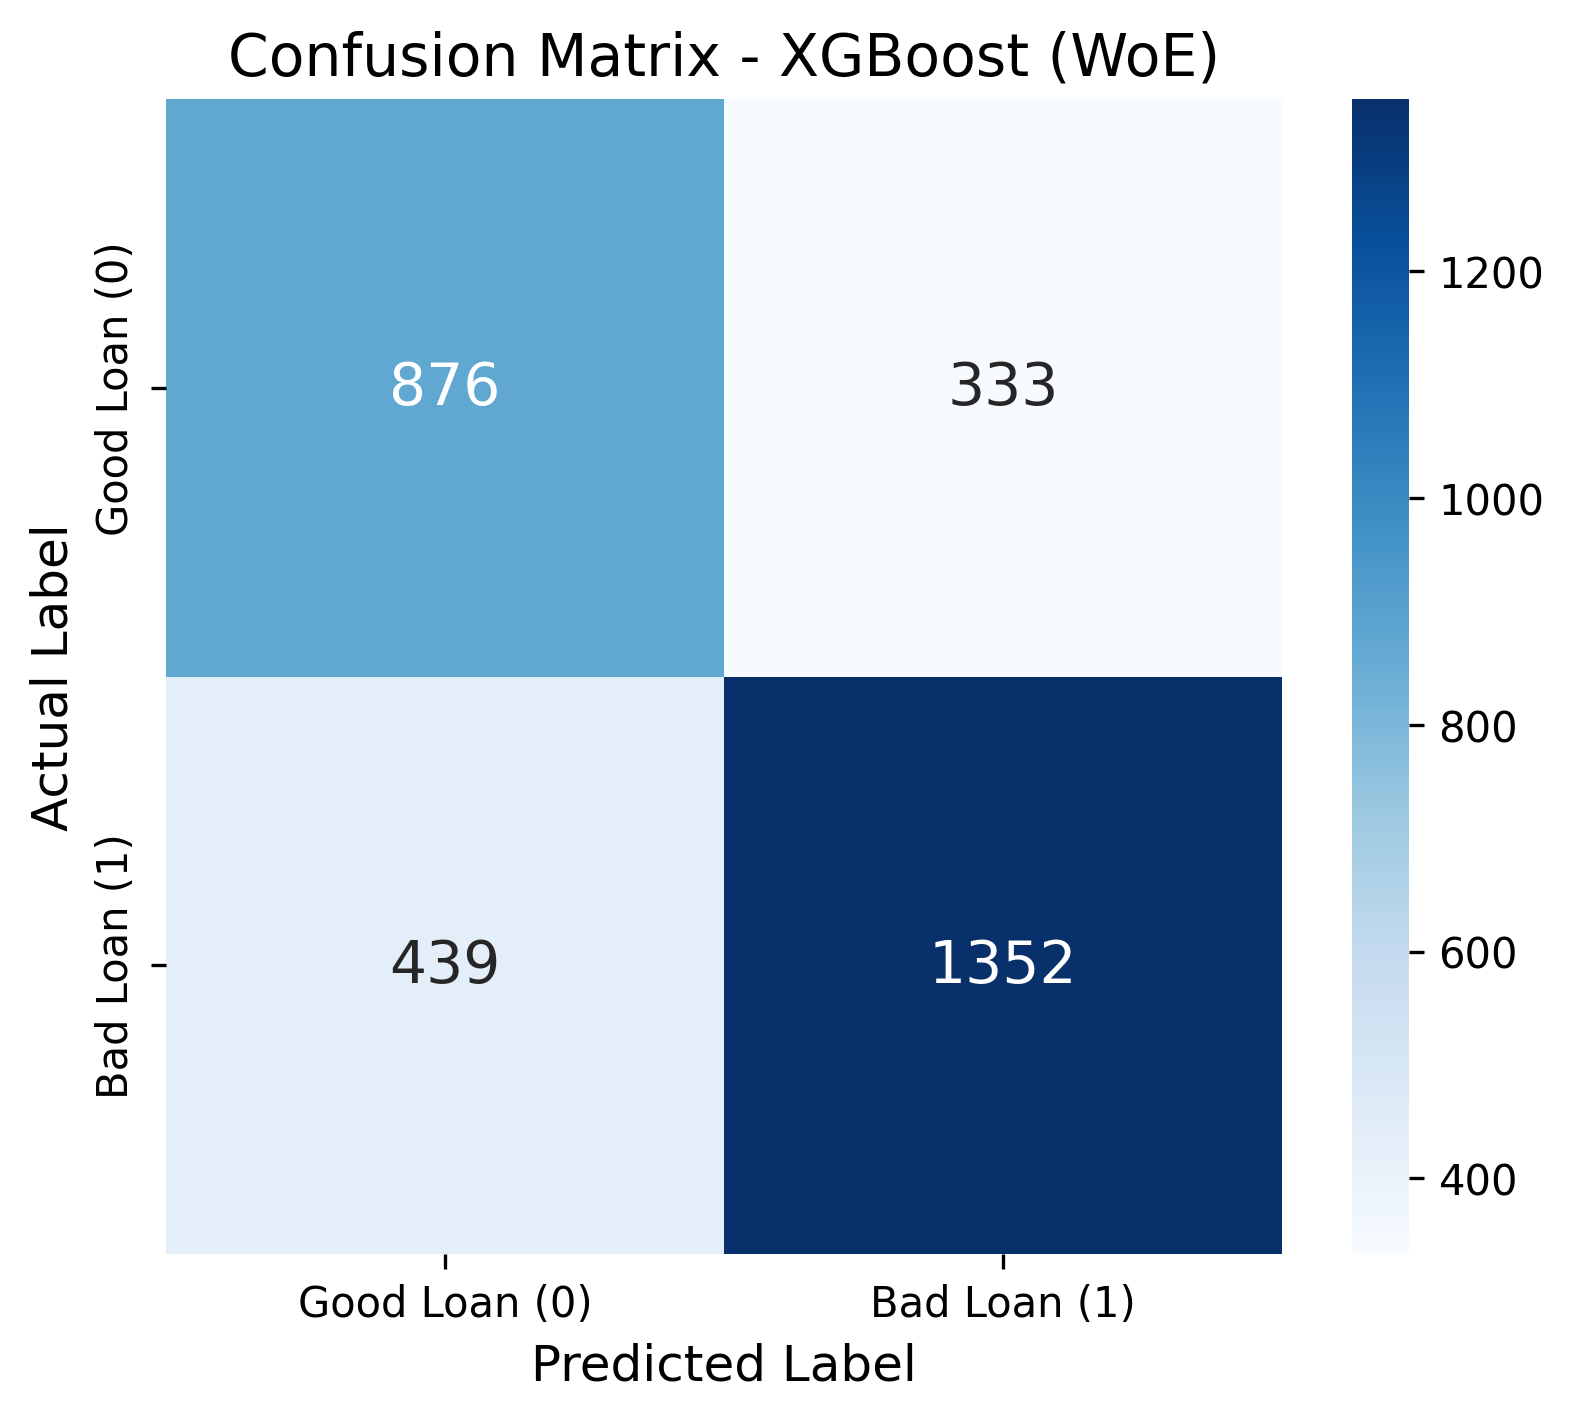
\includegraphics[width=0.62\textwidth]{bab4/Confusion_Matrix.png}
\caption{Confusion matrix hasil pengujian model klasifikasi risiko kredit}
\label{fig:bab4_confusion_matrix}
\end{figure}

Untuk menjelaskan keputusan model, penelitian ini menggunakan SHAP. Gambar \ref{fig:bab4_shap_summary} menunjukkan kontribusi fitur secara global terhadap prediksi model. Berdasarkan visualisasi tersebut, \textit{bureau\_score} menjadi salah satu fitur paling dominan. Skor biro kredit yang rendah cenderung meningkatkan probabilitas default, sedangkan skor yang tinggi cenderung menurunkan risiko. Hal ini sejalan dengan prinsip penilaian kredit, yaitu riwayat kredit menjadi indikator penting dalam menentukan kelayakan nasabah.

\begin{figure}[H]
\centering
\includegraphics[width=0.78\textwidth]{bab4/SHAP_Summary.png}
\caption{SHAP summary plot untuk interpretasi global model XGBoost}
\label{fig:bab4_shap_summary}
\end{figure}

Gambar \ref{fig:bab4_shap_summary_detail} menyajikan ringkasan kontribusi fitur dalam format lain. Visualisasi tambahan ini memperkuat analisis bahwa evaluasi model tidak hanya dilakukan melalui metrik numerik, tetapi juga melalui penjelasan faktor yang memengaruhi prediksi.

\begin{figure}[H]
\centering
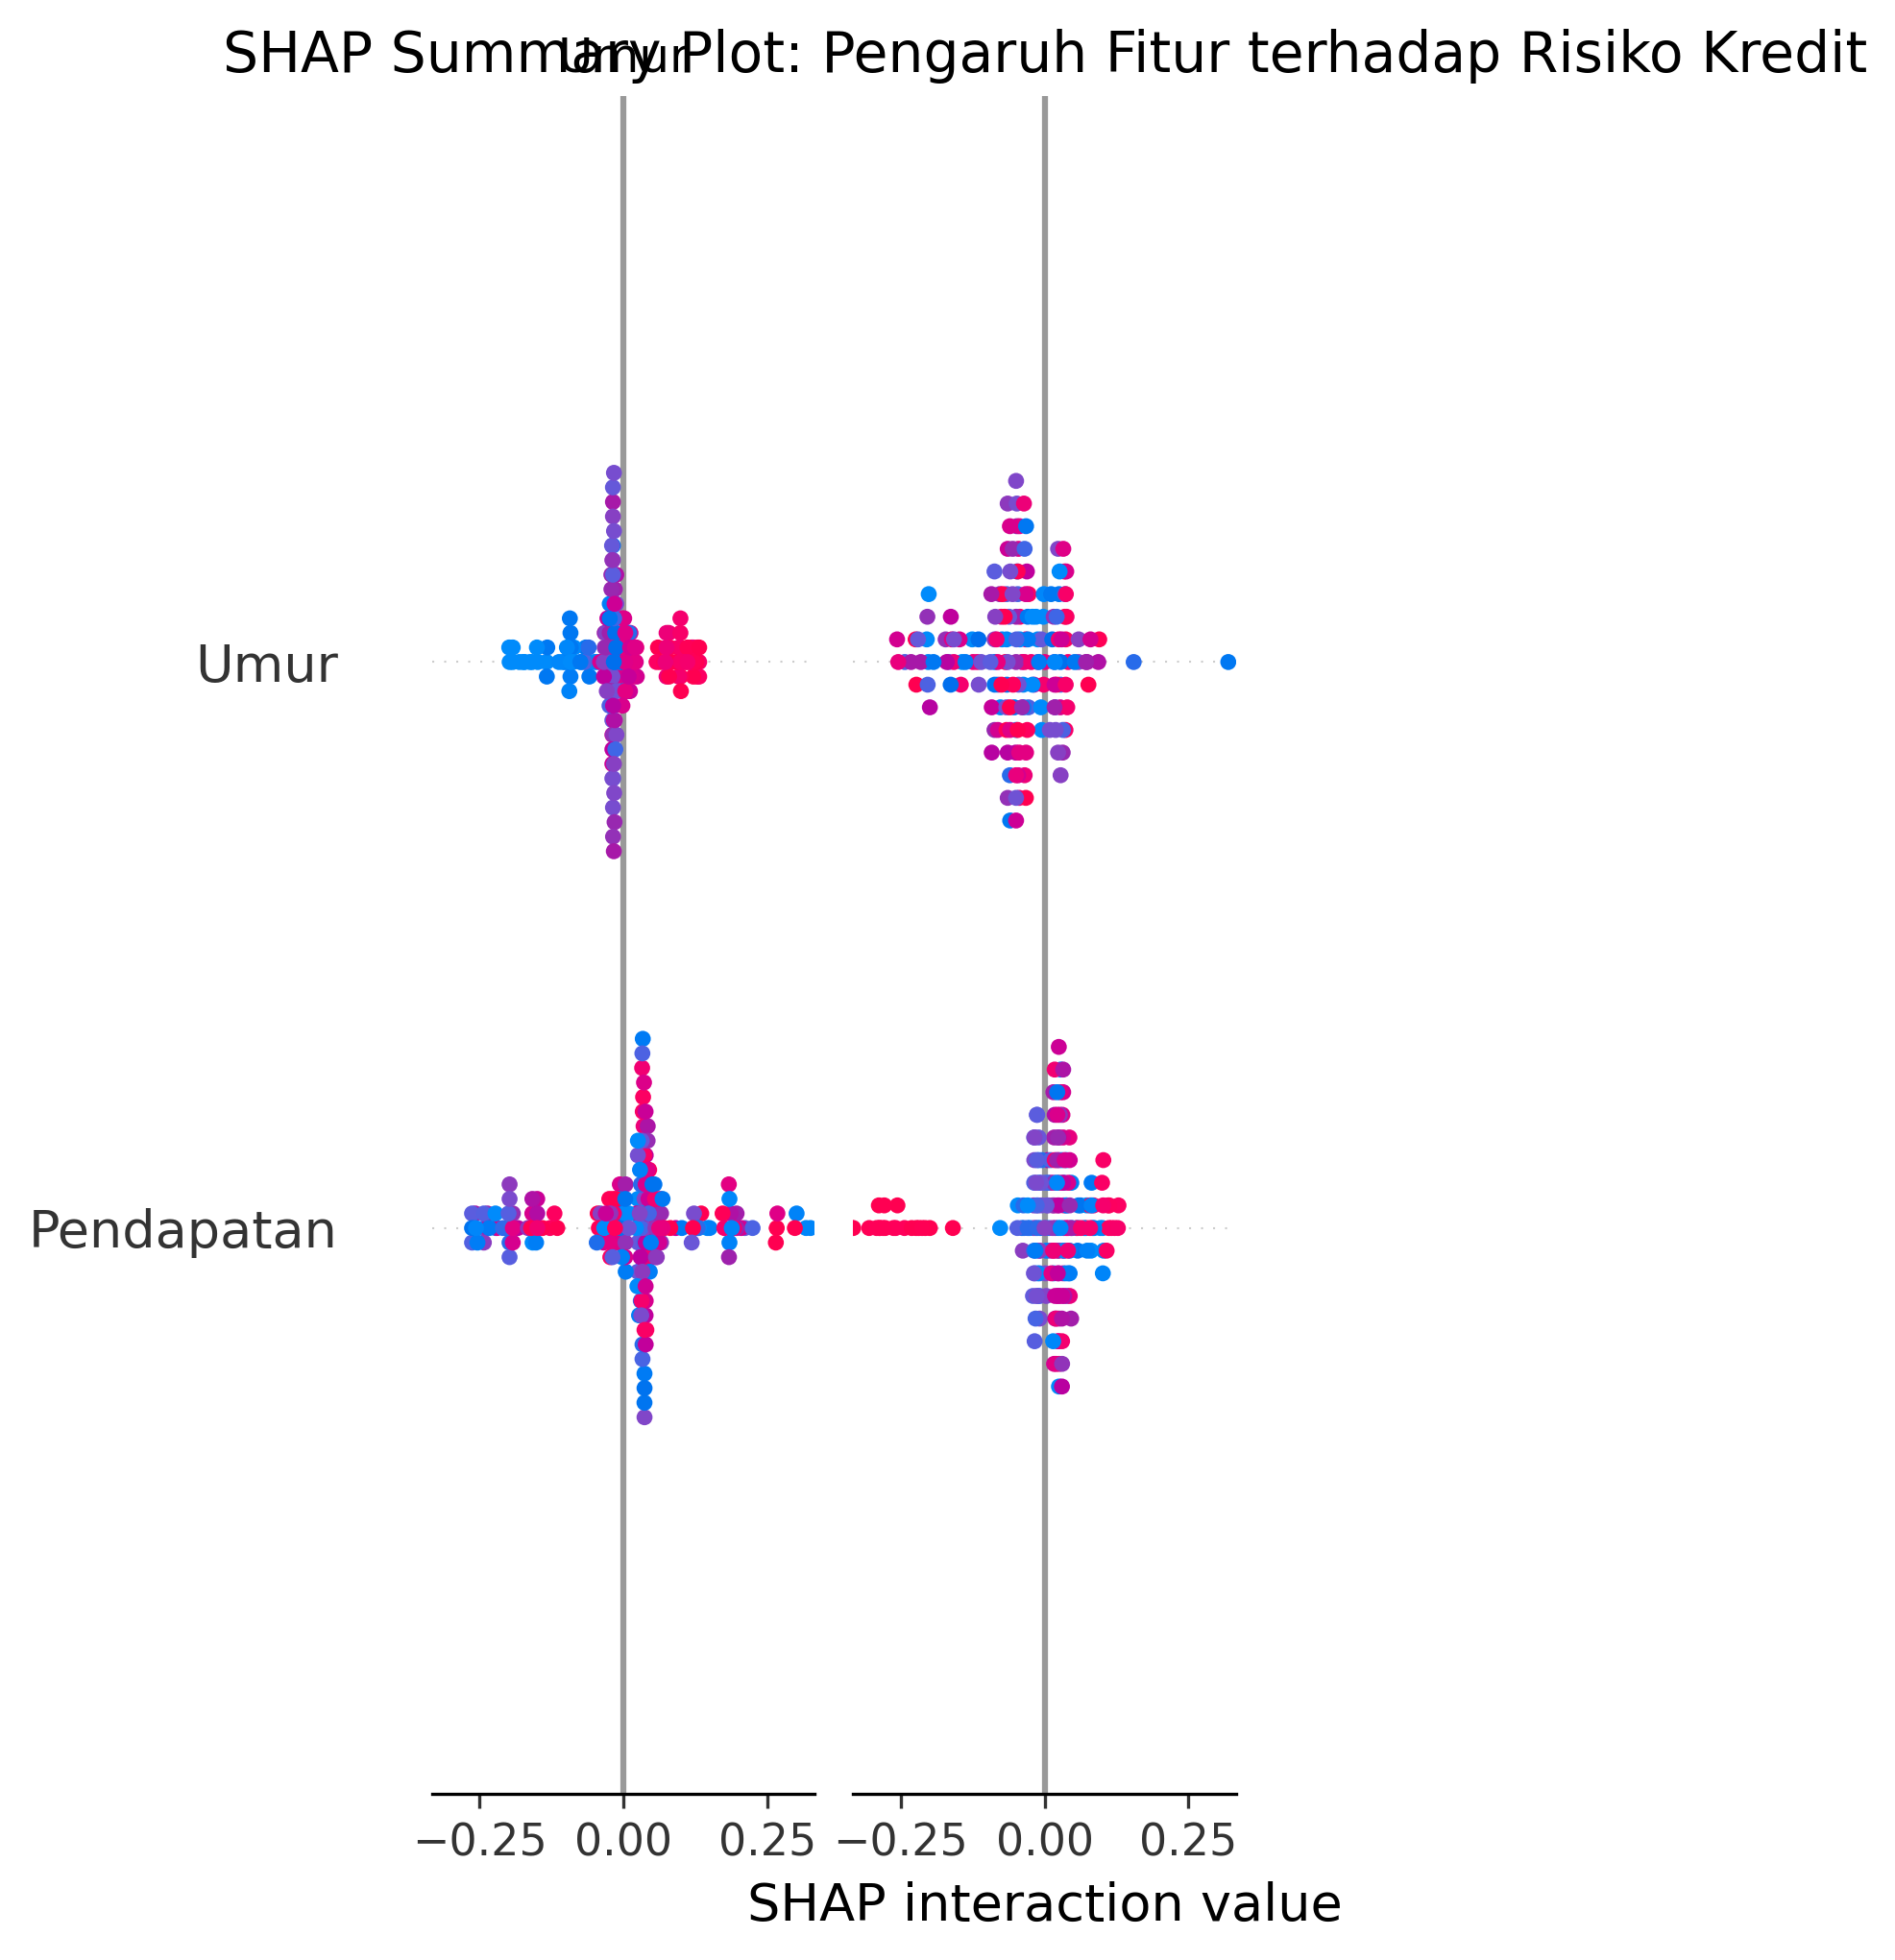
\includegraphics[width=0.76\textwidth]{bab4/shap_summary.png}
\caption{Ringkasan kontribusi fitur berdasarkan nilai SHAP}
\label{fig:bab4_shap_summary_detail}
\end{figure}


\section{Pengujian Perbandingan Skenario Model dan Studi Ablasi}
\label{sec:bab4_perbandingan_skenario}
Selain menguji model utama, penelitian ini juga melakukan studi ablasi (\textit{ablation study}) untuk mengevaluasi kontribusi transformasi \textit{Weight of Evidence} (WoE) dan penanganan ketidakseimbangan kelas menggunakan SMOTE. Studi ini dilakukan dengan membandingkan empat arsitektur model klasifikasi, yaitu Logistic Regression, Decision Tree, Random Forest, dan XGBoost.

Pengujian dilakukan pada empat konfigurasi data. Pertama, konfigurasi \textit{Full} menggunakan WoE dan SMOTE. Kedua, konfigurasi \textit{No SMOTE} menggunakan WoE tanpa penyeimbangan kelas. Ketiga, konfigurasi \textit{No WoE} menggunakan fitur mentah yang telah distandardisasi dan di-encode, kemudian diseimbangkan dengan SMOTE. Keempat, konfigurasi \textit{Raw} menggunakan fitur mentah tanpa WoE dan tanpa SMOTE. Perbandingan ini bertujuan melihat apakah peningkatan performa berasal dari model, transformasi fitur, penyeimbangan kelas, atau kombinasi ketiganya.

\begin{scriptsize}
\setlength{\tabcolsep}{3pt}
\renewcommand{\arraystretch}{1.1}
\begin{longtable}{p{0.18\textwidth} p{0.18\textwidth} c c c c c}
\caption{Perbandingan kinerja model dan studi ablasi}
\label{tab:bab4_ablation_study} \\
\toprule
\textbf{Konfigurasi Data} & \textbf{Arsitektur Model} & \textbf{ROC AUC} & \textbf{F1} & \textbf{Presisi} & \textbf{Recall} & \textbf{Waktu (s)} \\
\midrule
\endfirsthead
\multicolumn{7}{c}{{\tablename\ \thetable{} -- Lanjutan dari halaman sebelumnya}} \\
\toprule
\textbf{Konfigurasi Data} & \textbf{Arsitektur Model} & \textbf{ROC AUC} & \textbf{F1} & \textbf{Presisi} & \textbf{Recall} & \textbf{Waktu (s)} \\
\midrule
\endhead
\midrule
\multicolumn{7}{r}{{Bersambung ke halaman berikutnya...}} \\
\endfoot
\bottomrule
\endlastfoot
\textit{Full} (WoE + SMOTE) & Logistic Regression & 0,8098 & 0,7563 & 0,7996 & 0,7175 & 0,0193 \\
 & Decision Tree & 0,7961 & 0,7574 & 0,7865 & 0,7303 & 0,0146 \\
 & Random Forest & 0,8214 & 0,7739 & 0,8059 & 0,7443 & 0,4186 \\
 & \textbf{XGBoost} & \textbf{0,8284} & \textbf{0,7752} & \textbf{0,8055} & \textbf{0,7471} & \textbf{0,1652} \\
\midrule
\textit{No SMOTE} (WoE) & Logistic Regression & 0,8096 & 0,7899 & 0,7613 & 0,8208 & 0,0121 \\
 & Decision Tree & 0,8029 & 0,7775 & 0,7707 & 0,7845 & 0,0071 \\
 & Random Forest & 0,8249 & 0,8049 & 0,7433 & 0,8777 & 0,3622 \\
 & XGBoost & 0,8319 & 0,8069 & 0,7339 & 0,8961 & 0,1138 \\
\midrule
\textit{No WoE} (SMOTE) & Logistic Regression & 0,7813 & 0,7457 & 0,7855 & 0,7097 & 0,0115 \\
 & Decision Tree & 0,8021 & 0,7666 & 0,7985 & 0,7370 & 0,0273 \\
 & Random Forest & 0,8311 & 0,7737 & 0,8204 & 0,7320 & 0,6336 \\
 & XGBoost & 0,8379 & 0,7831 & 0,8181 & 0,7510 & 0,1277 \\
\midrule
\textit{Raw} & Logistic Regression & 0,7814 & 0,7705 & 0,7341 & 0,8107 & 0,0116 \\
 & Decision Tree & 0,8011 & 0,7712 & 0,7653 & 0,7772 & 0,0219 \\
 & Random Forest & 0,8224 & 0,7982 & 0,7428 & 0,8626 & 0,6064 \\
 & XGBoost & 0,8367 & 0,8071 & 0,7282 & 0,9051 & 0,2196 \\
\end{longtable}
\renewcommand{\arraystretch}{1}
\end{scriptsize}

Secara visual, perbandingan kurva ROC antararsitektur model pada konfigurasi utama ditunjukkan pada Gambar \ref{fig:bab4_roc_comparison}. Visualisasi ini digunakan untuk melihat kemampuan diskriminasi masing-masing model pada berbagai ambang keputusan.

\begin{figure}[H]
\centering
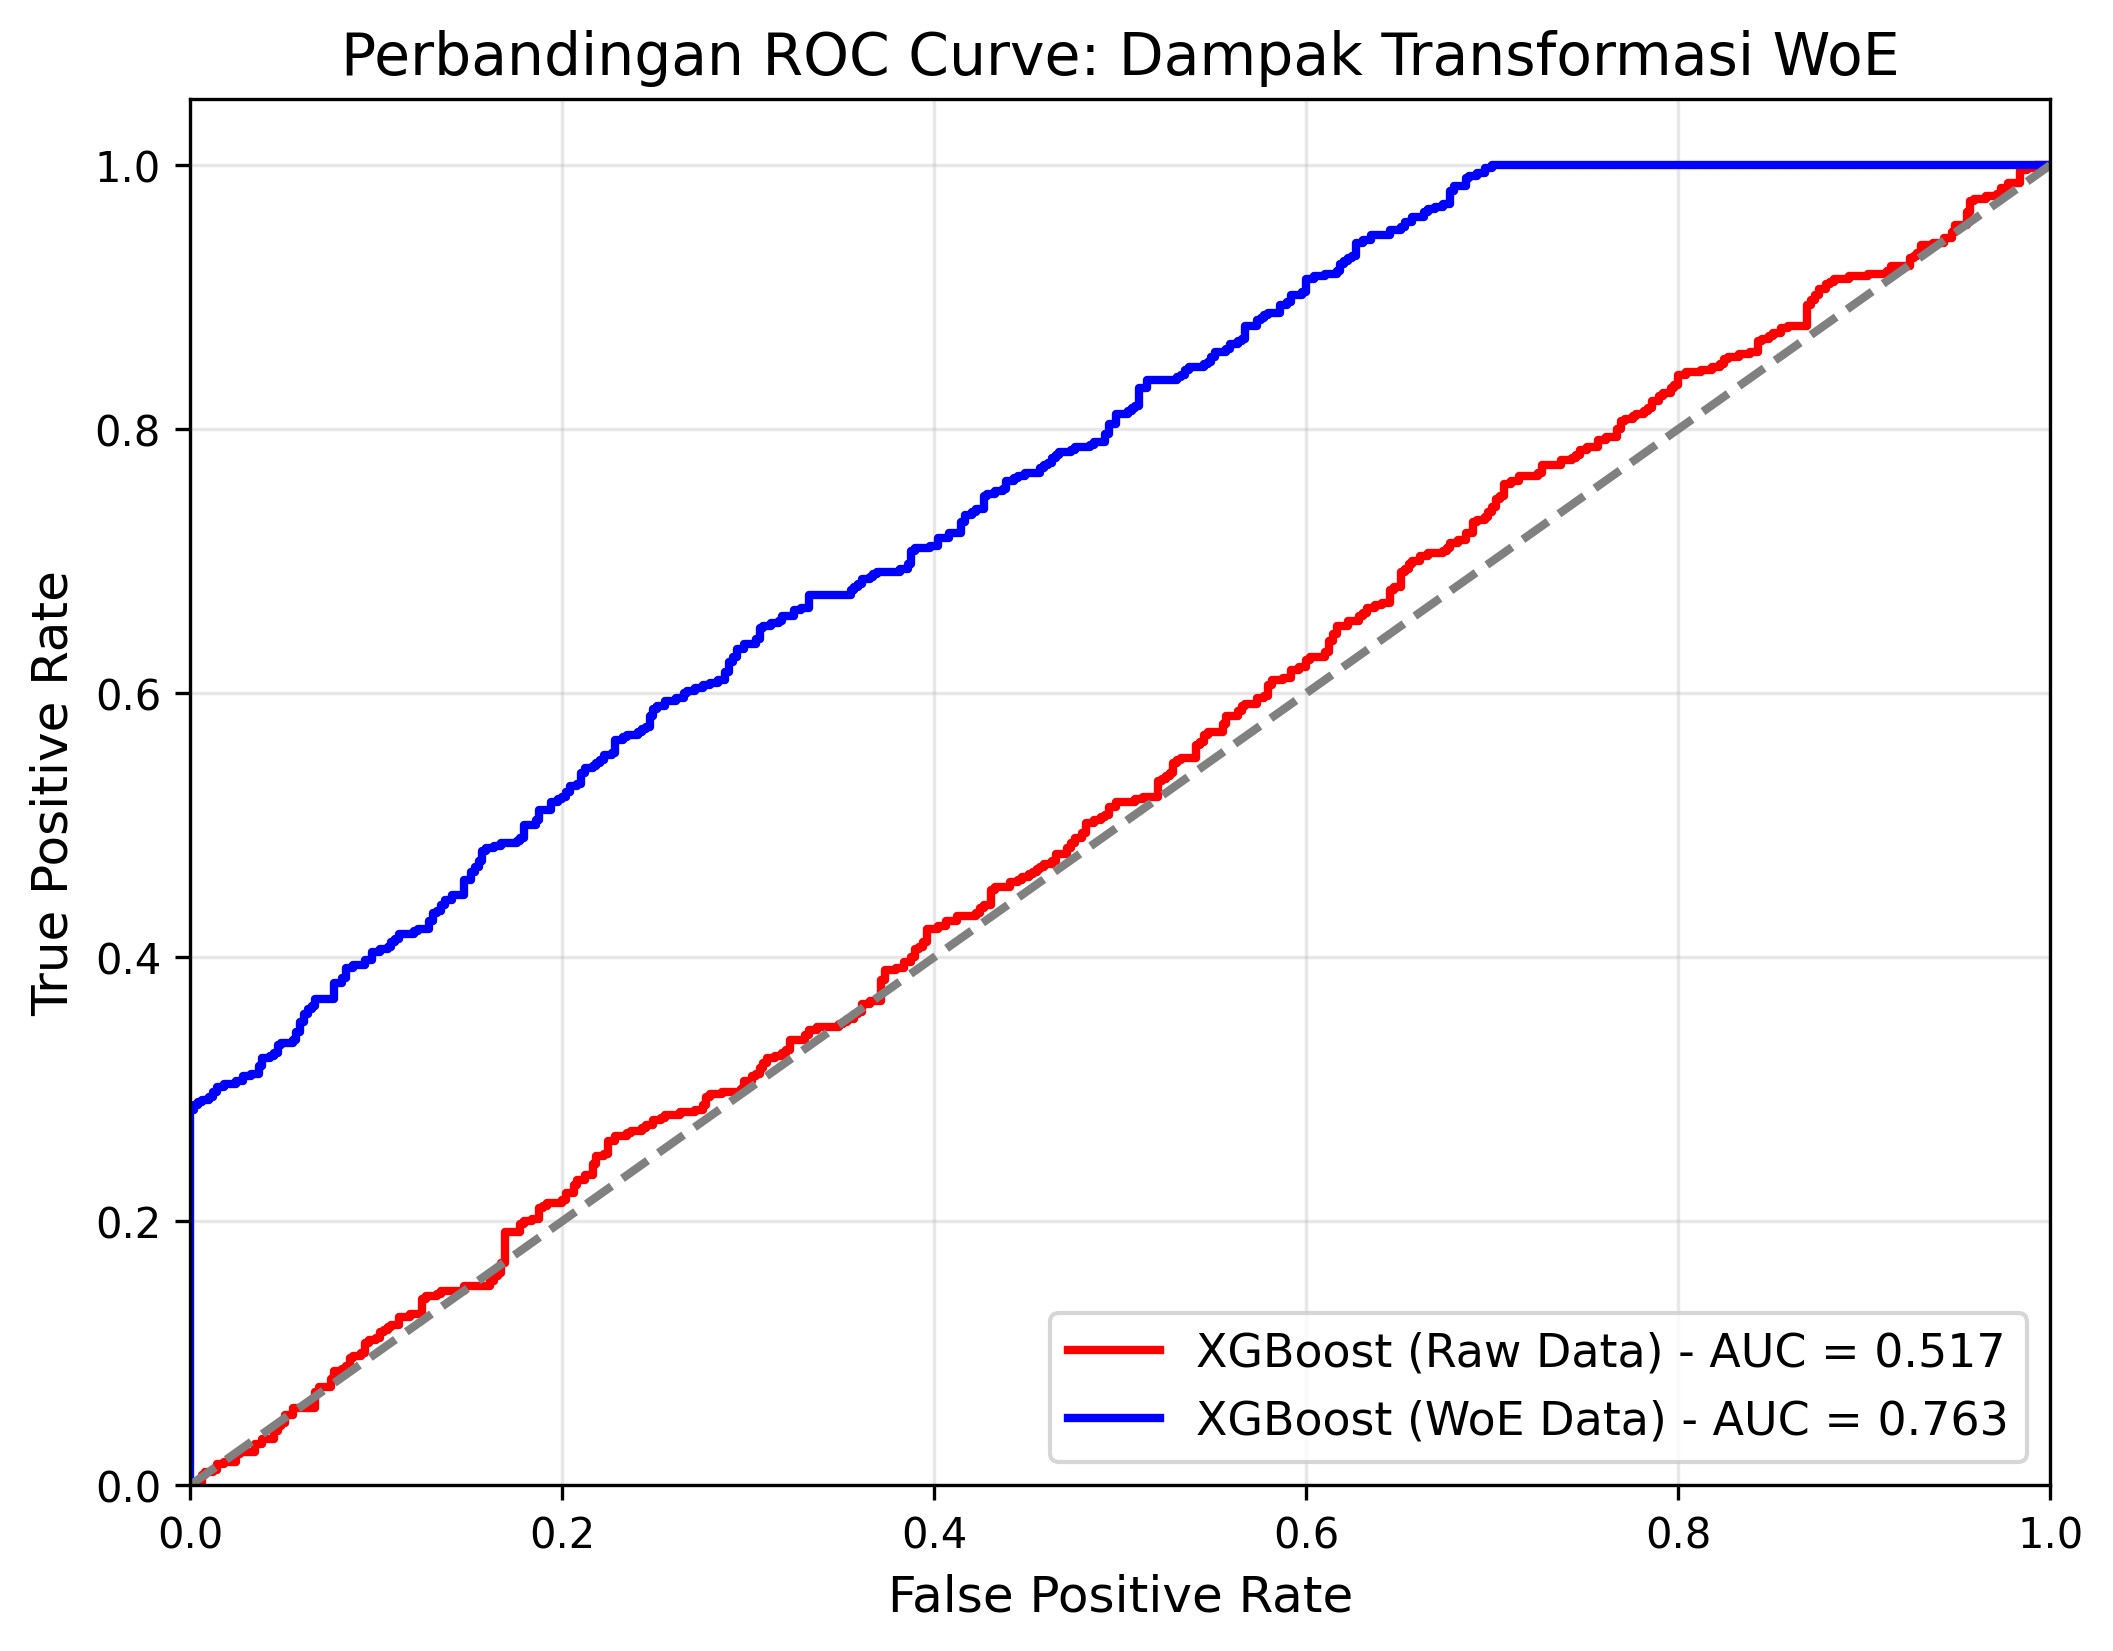
\includegraphics[width=0.8\textwidth]{bab4/roc_curve_comparison.png}
\caption{Perbandingan kurva ROC antara model dan skenario pengujian}
\label{fig:bab4_roc_comparison}
\end{figure}

\subsection{Analisis Dampak Transformasi Weight of Evidence}
Hasil studi ablasi menunjukkan bahwa transformasi WoE memberikan dampak yang berbeda antara model linear dan model berbasis pohon. Pada Logistic Regression, penggunaan WoE meningkatkan ROC AUC dari 0,7813 pada skenario \textit{No WoE} menjadi 0,8098 pada skenario \textit{Full}. Peningkatan ini terjadi karena WoE memetakan hubungan antara fitur dan peluang gagal bayar ke dalam bentuk yang lebih dekat dengan relasi log-odds, sehingga lebih sesuai dengan karakteristik model linear.

Pada model non-linear seperti XGBoost dan Random Forest, peniadaan WoE tidak selalu menurunkan ROC AUC. XGBoost pada skenario \textit{No WoE} memperoleh ROC AUC 0,8379, sedikit lebih tinggi dibandingkan skenario \textit{Full} sebesar 0,8284. Hal ini wajar karena model berbasis pohon mampu menangkap hubungan non-linear secara langsung dari fitur mentah. Namun, WoE tetap penting dalam konteks risiko kredit karena menghasilkan fitur yang lebih stabil, lebih mudah diaudit, dan lebih mudah dijelaskan kepada analis maupun pihak pengawas.

\subsection{Analisis Dampak SMOTE}
Penerapan SMOTE mengubah keseimbangan antara presisi dan recall model. Pada XGBoost dengan WoE tanpa SMOTE, recall mencapai 0,8961 tetapi presisi hanya 0,7339. Setelah SMOTE diterapkan pada konfigurasi \textit{Full}, presisi meningkat menjadi 0,8055, sedangkan recall menjadi 0,7471. Perubahan ini menunjukkan bahwa SMOTE menggeser batas keputusan model agar prediksi default menjadi lebih selektif dan tidak terlalu banyak menghasilkan peringatan risiko yang keliru.

Dalam konteks bisnis, peningkatan presisi penting karena dapat mengurangi kesalahan dalam menandai nasabah layak sebagai berisiko tinggi. Di sisi lain, recall 0,7471 masih menunjukkan bahwa model tetap mampu mendeteksi sebagian besar nasabah yang berpotensi gagal bayar. Oleh karena itu, konfigurasi \textit{Full} dipilih sebagai skenario yang lebih seimbang antara akurasi prediktif, stabilitas fitur, interpretabilitas, dan kebutuhan operasional.

\subsection{Analisis Interpretabilitas SHAP Lintas Model}
Untuk mengevaluasi konsistensi penjelasan model, dilakukan analisis SHAP pada konfigurasi \textit{Full}. Gambar \ref{fig:bab4_shap_lr} sampai Gambar \ref{fig:bab4_shap_xgb} menunjukkan ringkasan kontribusi fitur untuk Logistic Regression, Decision Tree, Random Forest, dan XGBoost.

\begin{figure}[H]
\centering
\begin{minipage}{0.48\textwidth}
\centering
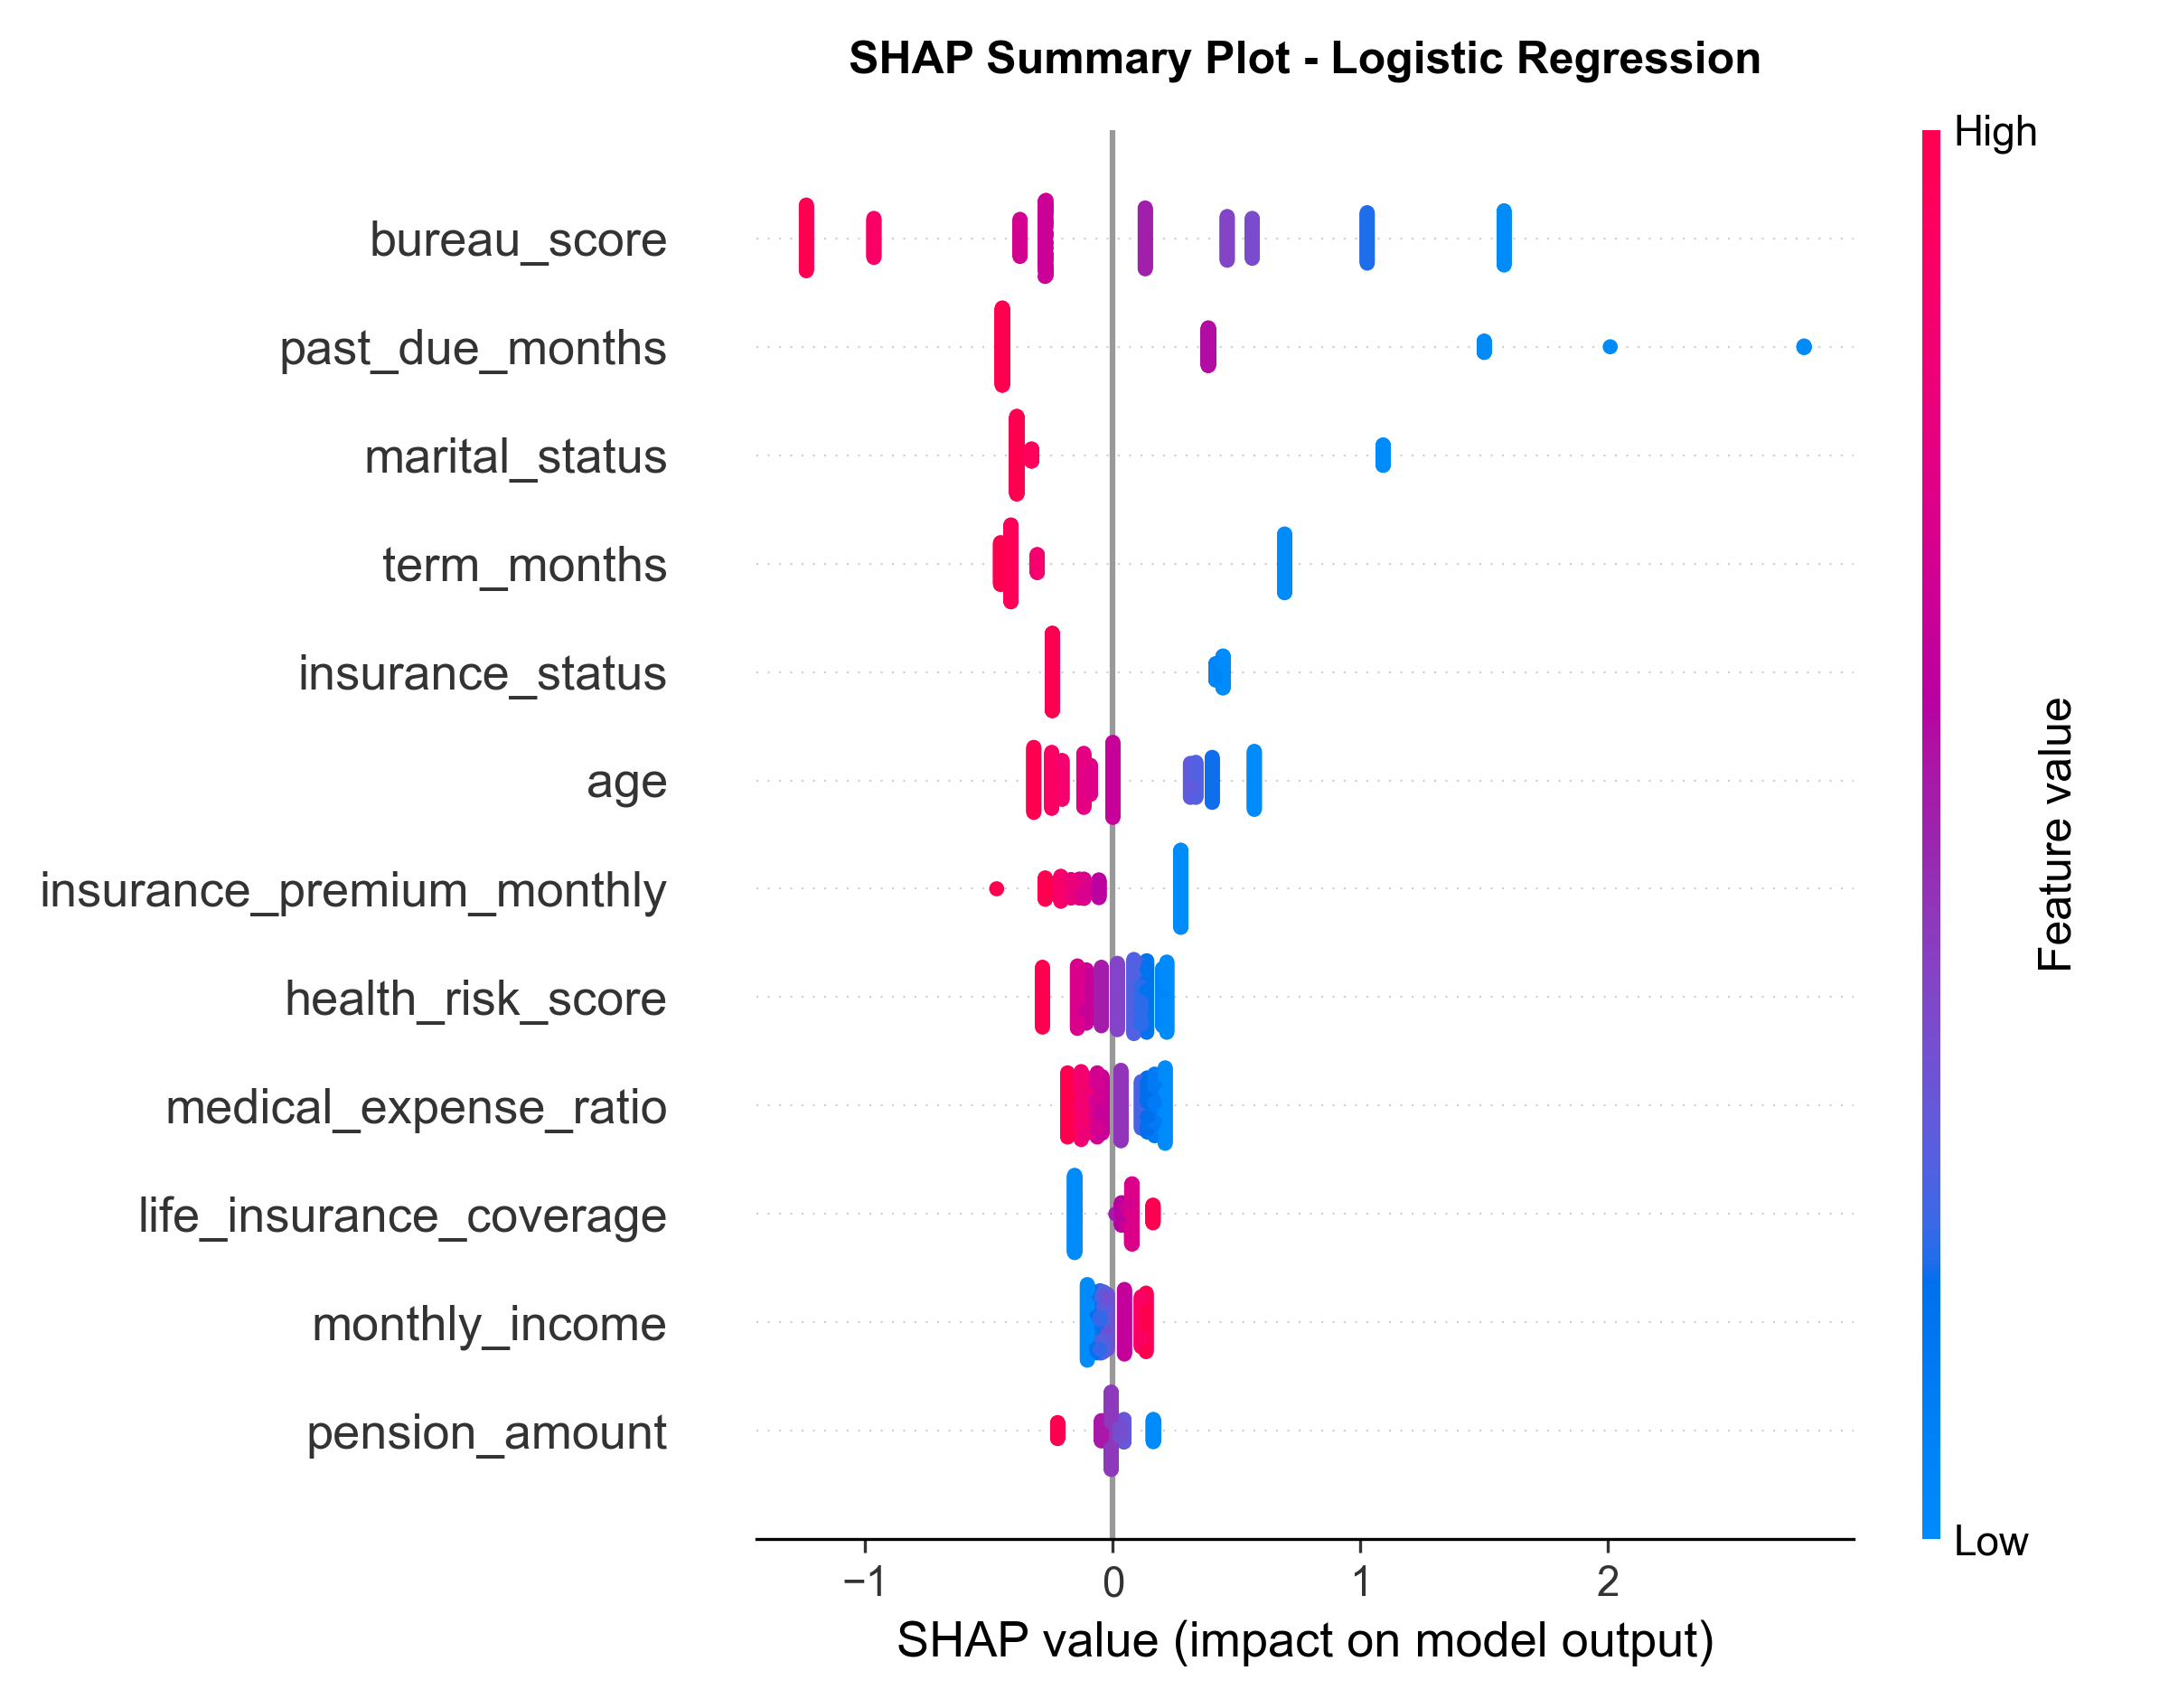
\includegraphics[width=\textwidth]{bab4/SHAP_Summary_LogisticRegression.png}
\caption{SHAP summary Logistic Regression}
\label{fig:bab4_shap_lr}
\end{minipage}
\hfill
\begin{minipage}{0.48\textwidth}
\centering
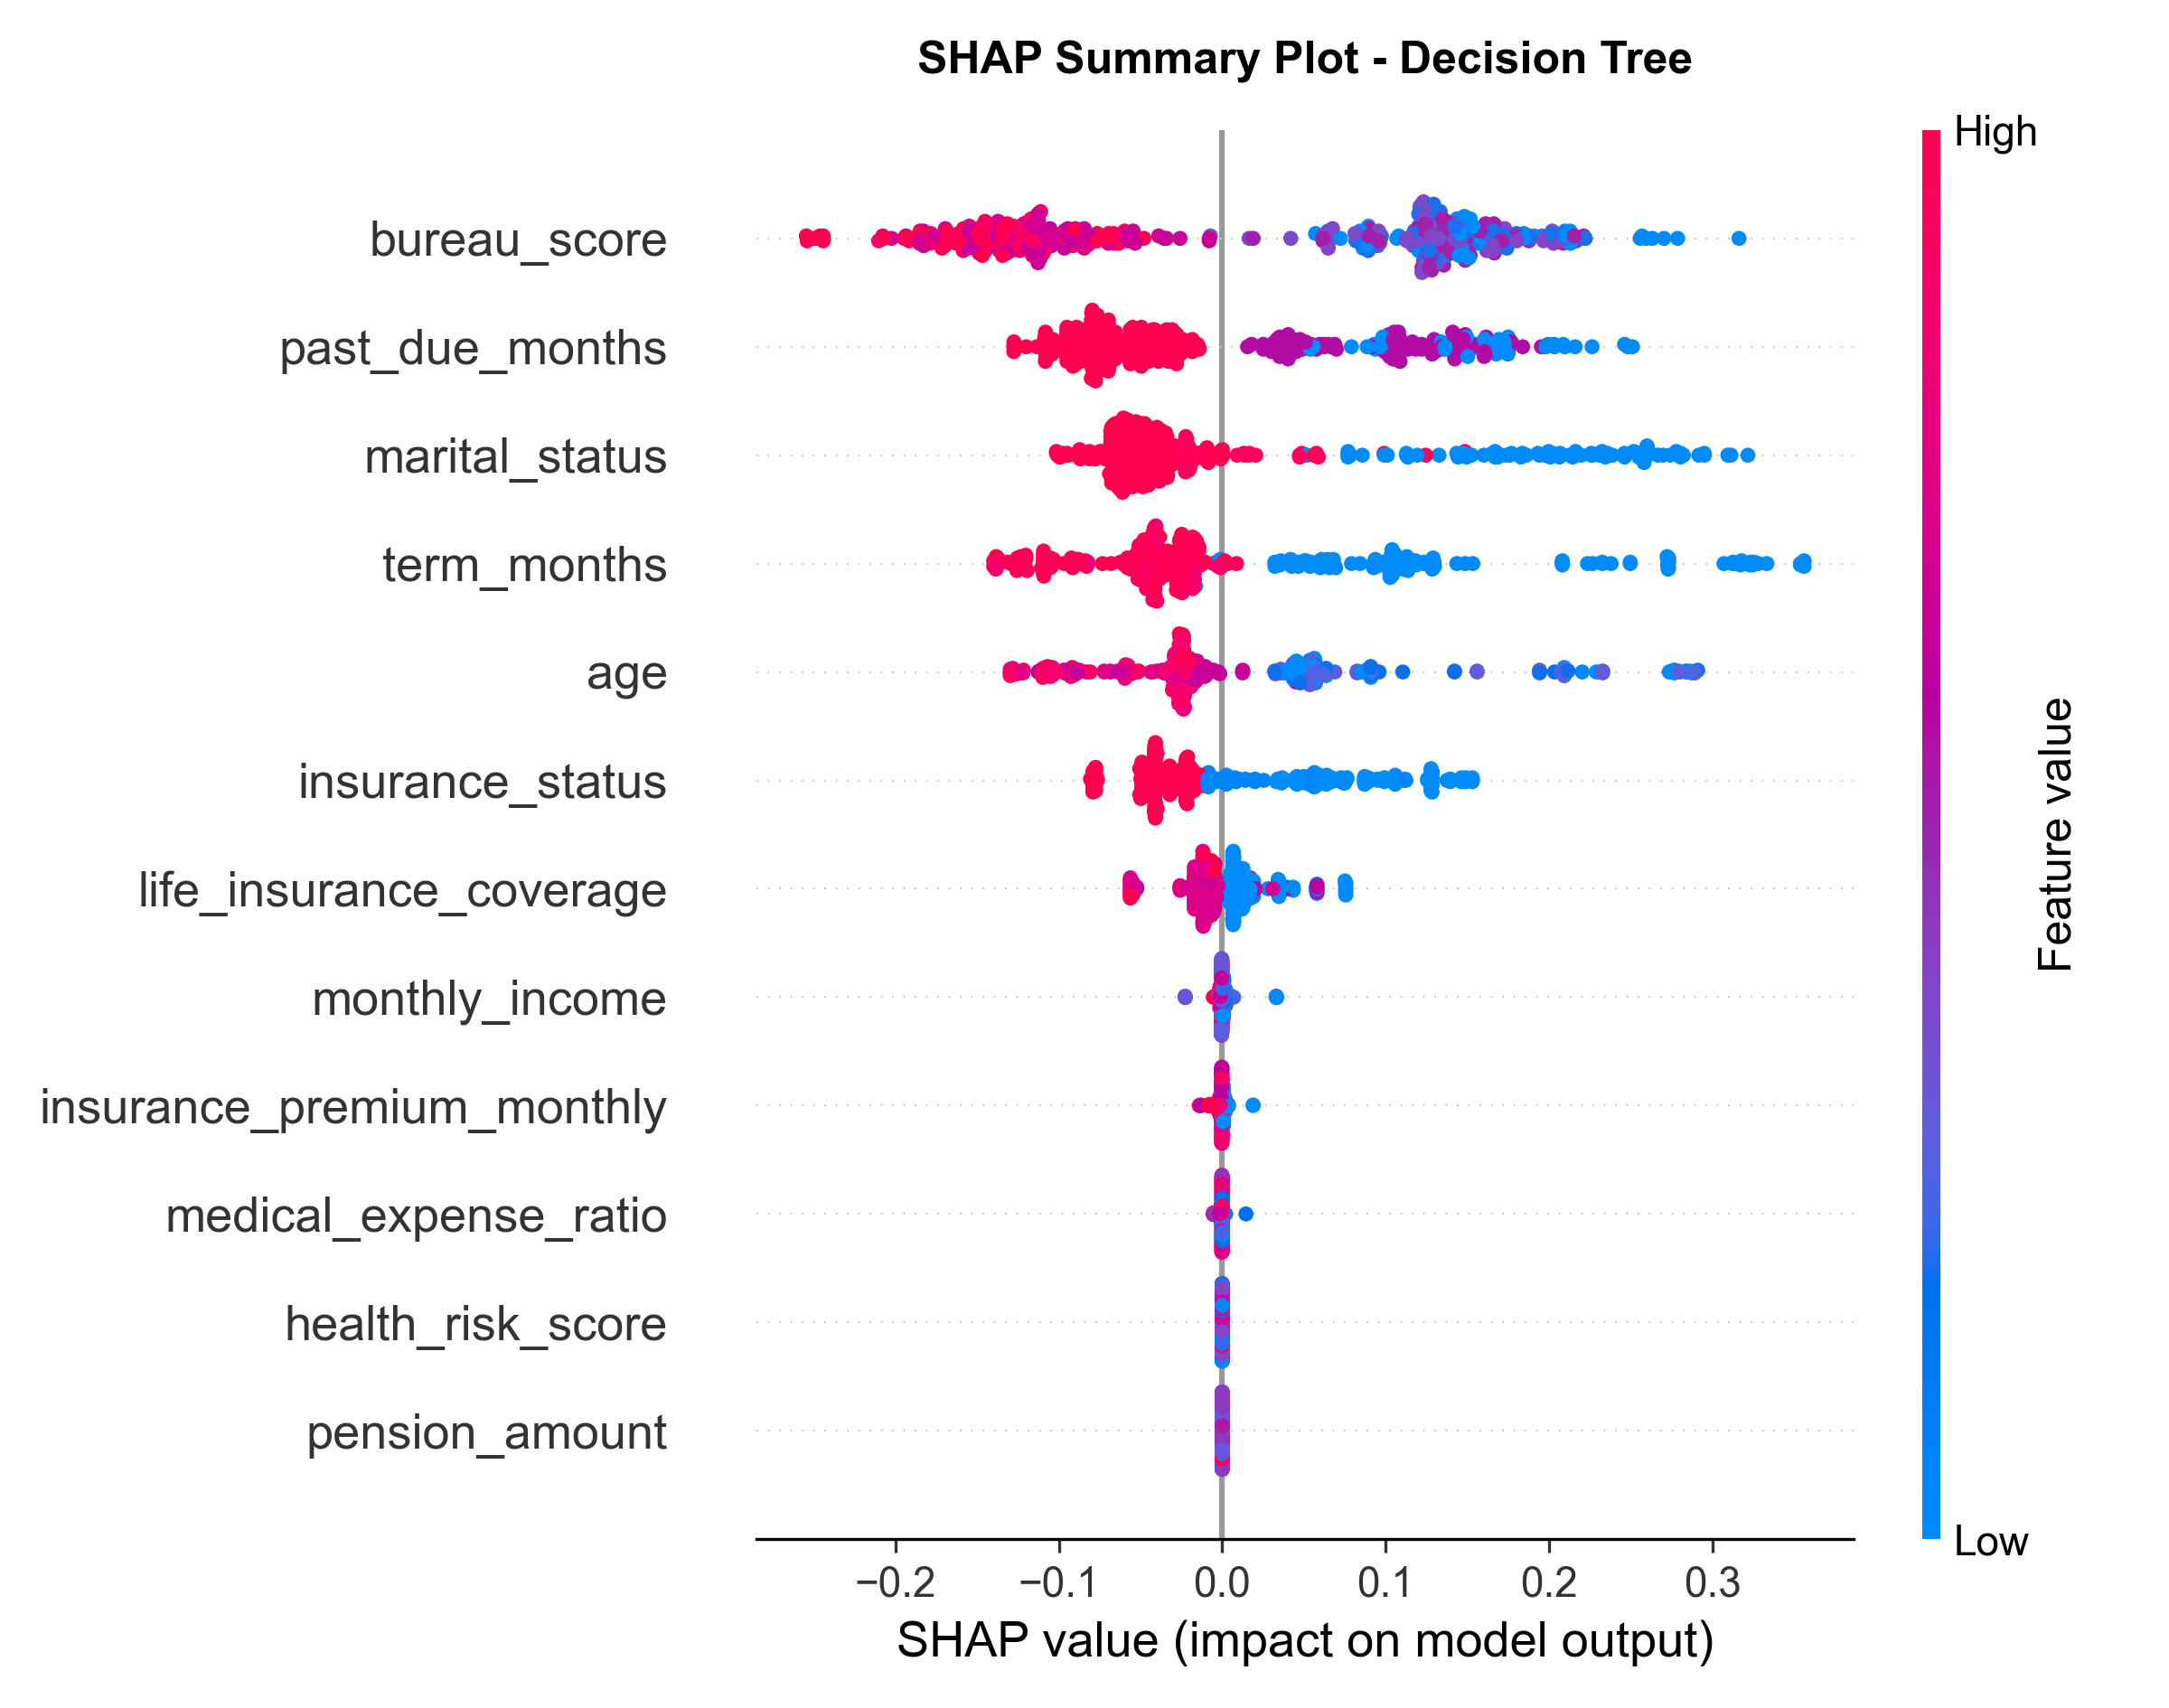
\includegraphics[width=\textwidth]{bab4/SHAP_Summary_DecisionTree.png}
\caption{SHAP summary Decision Tree}
\label{fig:bab4_shap_dt}
\end{minipage}
\end{figure}

\begin{figure}[H]
\centering
\begin{minipage}{0.48\textwidth}
\centering
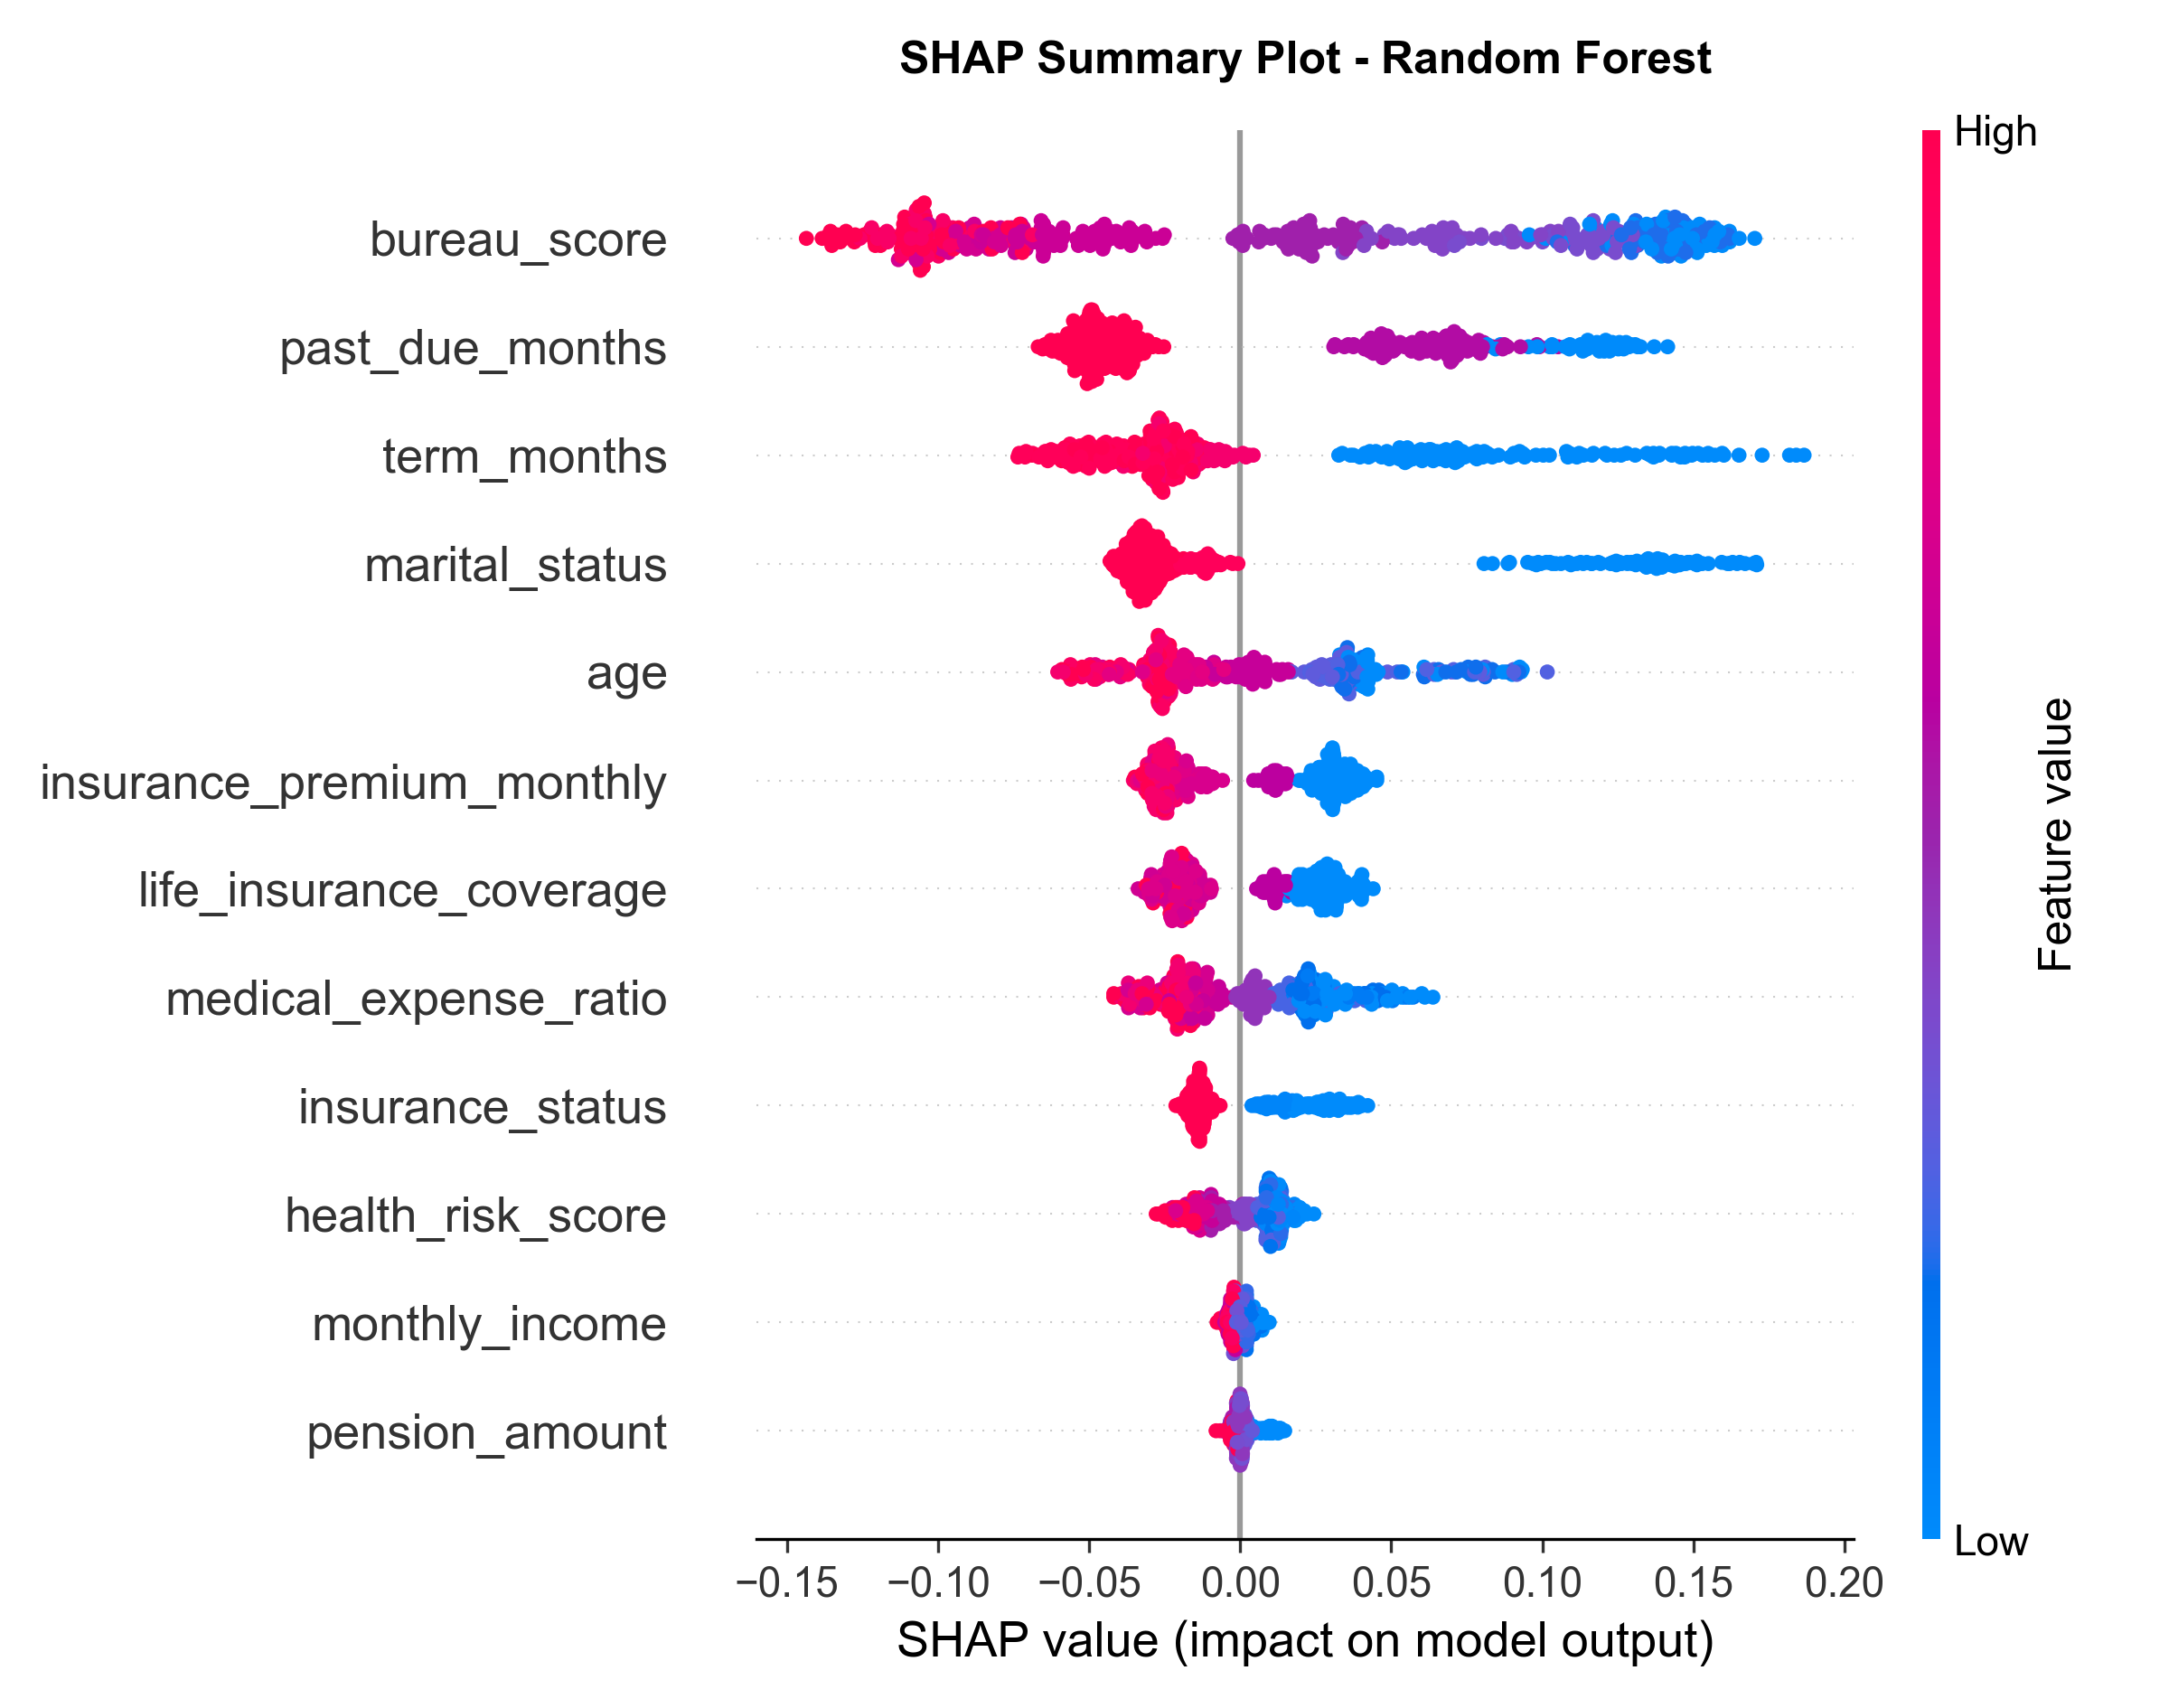
\includegraphics[width=\textwidth]{bab4/SHAP_Summary_RandomForest.png}
\caption{SHAP summary Random Forest}
\label{fig:bab4_shap_rf}
\end{minipage}
\hfill
\begin{minipage}{0.48\textwidth}
\centering
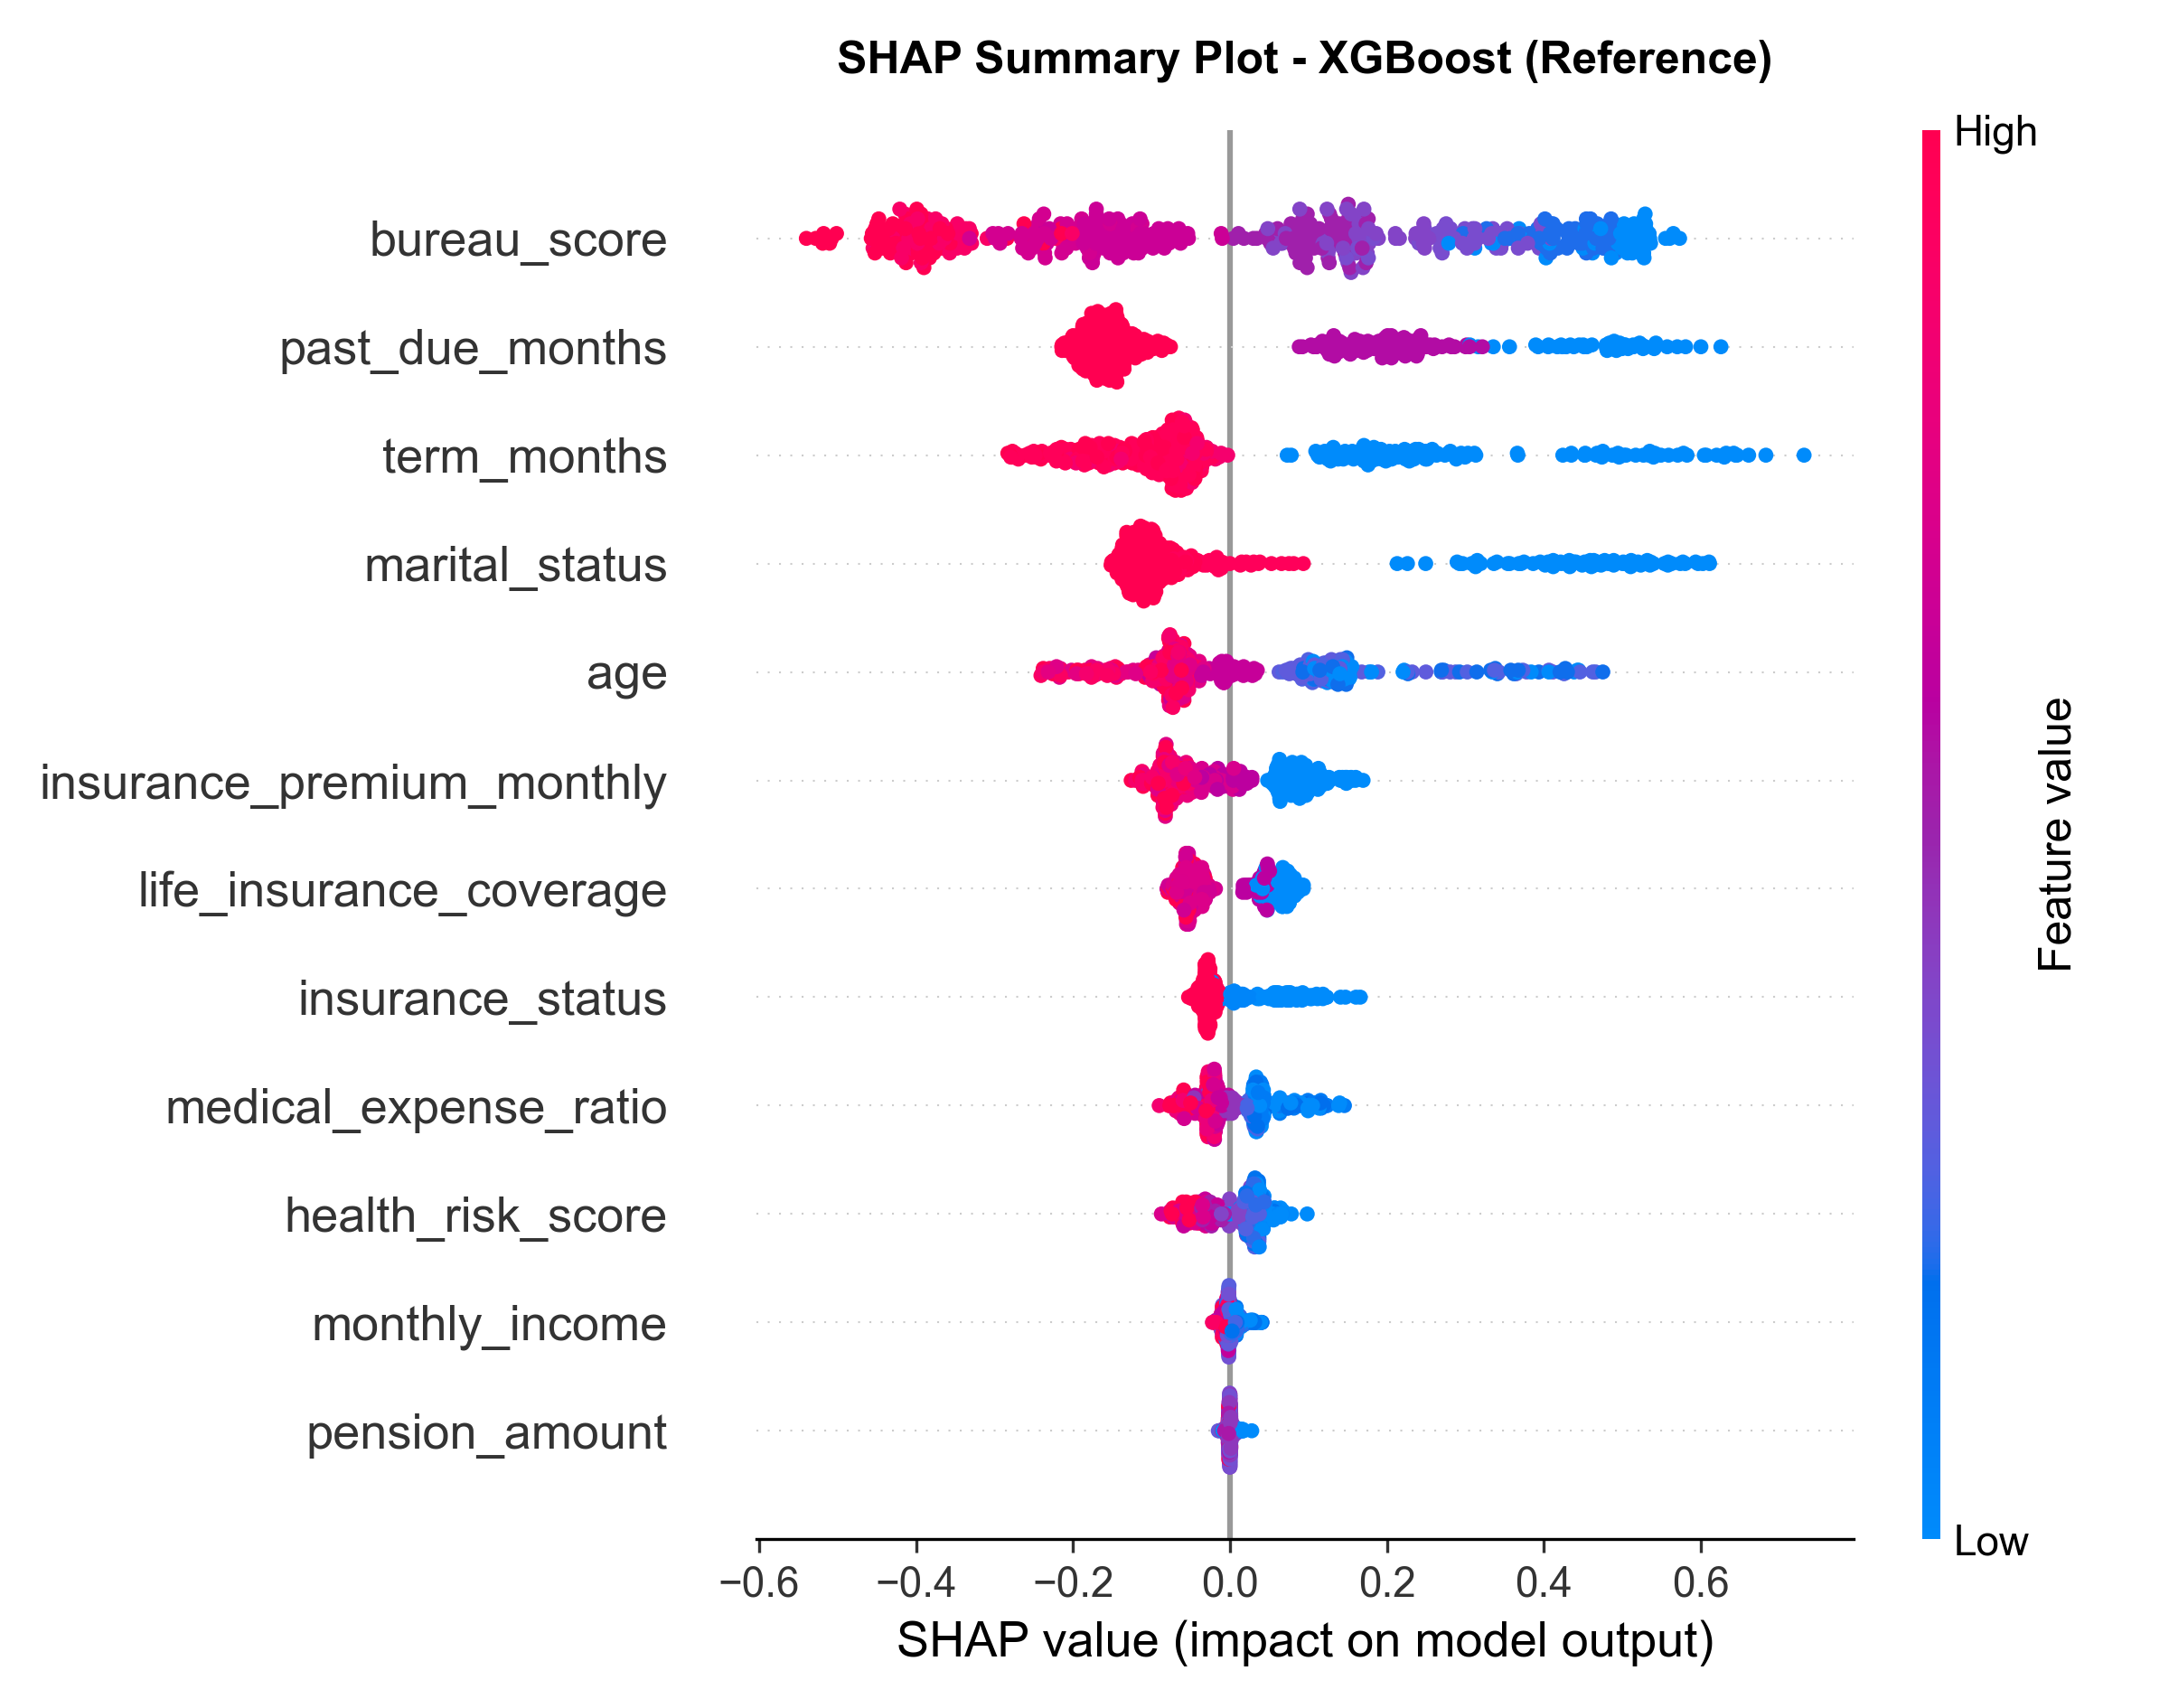
\includegraphics[width=\textwidth]{bab4/SHAP_Summary_XGBoost.png}
\caption{SHAP summary XGBoost}
\label{fig:bab4_shap_xgb}
\end{minipage}
\end{figure}

Hasil interpretasi menunjukkan bahwa \textit{bureau\_score} menjadi fitur paling dominan pada seluruh model. Fitur \textit{past\_due\_months} juga konsisten berada pada peringkat atas, yang menunjukkan bahwa histori keterlambatan pembayaran merupakan sinyal penting dalam memprediksi gagal bayar. Selain itu, \textit{marital\_status} dan \textit{term\_months} memberikan pengaruh menengah, sedangkan fitur seperti \textit{monthly\_income} dan \textit{pension\_amount} berperan sebagai penyesuaian tambahan terhadap profil risiko nasabah.

Konsistensi kontribusi fitur antar model menunjukkan bahwa pipeline berbasis WoE tidak hanya menghasilkan performa prediktif yang kompetitif, tetapi juga menjaga koherensi interpretasi. Dengan demikian, penggunaan XGBoost sebagai model referensi tetap dapat dijustifikasi karena hasil prediksinya selaras dengan faktor risiko yang logis dalam konteks penilaian kredit.

\section{Pengujian API Serving dan Aturan Bisnis}
\label{sec:bab4_api_serving}
Model terbaik yang telah dipilih kemudian diuji melalui layanan FastAPI pada endpoint \textit{/predict}. Pengujian ini bertujuan memastikan bahwa model dapat menerima input dalam format JSON, mengembalikan skor risiko, menghasilkan grade, serta menyertakan penjelasan berbasis SHAP untuk mendukung transparansi keputusan.

Pada kasus uji pertama, nasabah berusia 48 tahun dengan \textit{bureau\_score} 750, pendapatan bulanan Rp8.500.000, tenor 24 bulan, DTI 0,25, dan tidak memiliki tunggakan diprediksi memiliki probabilitas gagal bayar sebesar 0,0845. Sistem mengembalikan Grade A, yang menunjukkan bahwa nasabah tergolong sangat layak. Nilai SHAP menunjukkan bahwa \textit{bureau\_score} dan \textit{insurance\_status} berkontribusi dalam menurunkan risiko.

\begin{table}[H]
\centering
\caption{Hasil pengujian API untuk nasabah normal}
\label{tab:bab4_api_normal}
\begin{tabular}{|l|l|}
\hline
\textbf{Aspek} & \textbf{Hasil} \\
\hline
Usia & 48 tahun \\
\hline
Bureau score & 750 \\
\hline
DTI & 0,25 \\
\hline
Probabilitas default & 0,0845 \\
\hline
Grade & A \\
\hline
Interpretasi & Nasabah sangat layak karena risiko gagal bayar rendah. \\
\hline
\end{tabular}
\end{table}

Pada kasus uji kedua, sistem diuji dengan aturan bisnis batas usia pelunasan maksimal 80 tahun. Nasabah berusia 75 tahun mengajukan tenor 120 bulan, sehingga usia saat pelunasan menjadi 85 tahun. Walaupun model memprediksi probabilitas gagal bayar rendah, yaitu 0,0214, sistem tetap menetapkan Grade Undefined karena permohonan melanggar aturan bisnis keras.

\begin{table}[H]
\centering
\caption{Hasil pengujian API untuk pelanggaran aturan usia pelunasan}
\label{tab:bab4_api_rule}
\begin{tabular}{|l|l|}
\hline
\textbf{Aspek} & \textbf{Hasil} \\
\hline
Usia awal & 75 tahun \\
\hline
Tenor & 120 bulan \\
\hline
Usia saat pelunasan & 85 tahun \\
\hline
Probabilitas model & 0,0214 \\
\hline
Output akhir & Grade Undefined \\
\hline
Alasan anomali & Usia saat pelunasan melebihi batas 80 tahun. \\
\hline
\end{tabular}
\end{table}

Hasil ini membuktikan bahwa sistem tidak hanya mengandalkan model machine learning, tetapi juga menerapkan aturan bisnis yang bersifat wajib. Dalam konteks perbankan, mekanisme seperti ini penting karena keputusan kredit tidak boleh sepenuhnya diserahkan pada model statistik ketika terdapat batasan regulasi atau kebijakan internal yang harus dipatuhi.

Antarmuka web yang digunakan untuk menguji layanan prediksi ditunjukkan pada Gambar \ref{fig:bab4_web_prediction}. Tampilan tersebut memperlihatkan bahwa pengguna dapat memasukkan atribut calon nasabah, seperti \textit{bureau score}, usia, status pernikahan, tipe pekerjaan, nilai pinjaman, dan tenor. Setelah tombol analisis dijalankan, sistem menampilkan probabilitas gagal bayar, grade risiko, serta daftar kontribusi fitur berbasis SHAP. Hasil ini menunjukkan bahwa layanan FastAPI tidak hanya dapat dipanggil secara teknis, tetapi juga dapat diintegrasikan ke dalam antarmuka pengguna yang lebih mudah dipahami oleh analis kredit.

\begin{figure}[H]
\centering
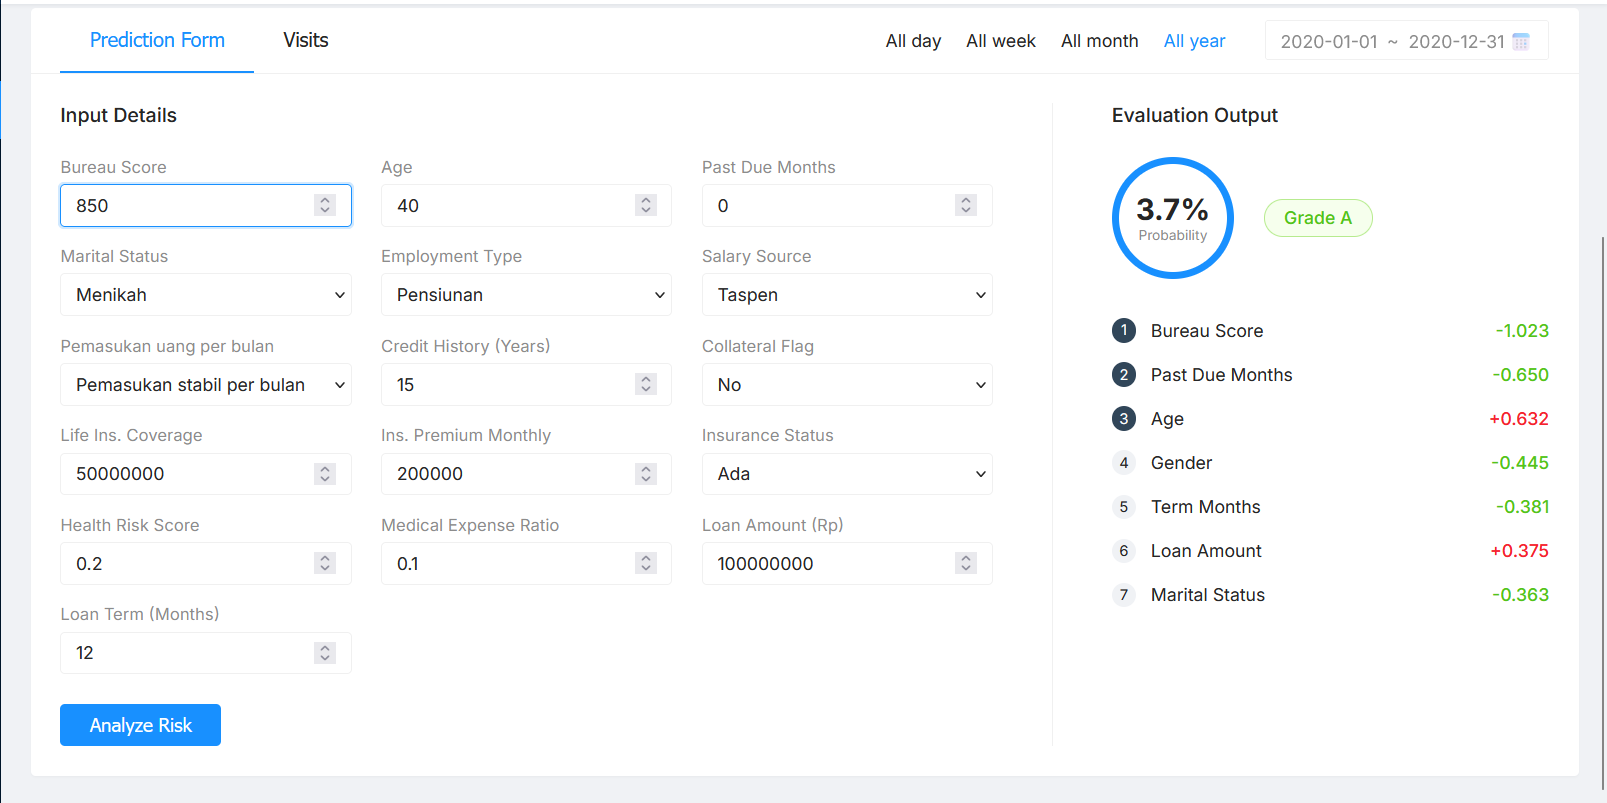
\includegraphics[width=0.92\textwidth]{bab4/Screenshot 2026-05-25 171508.png}
\caption{Antarmuka web untuk pengujian prediksi risiko kredit}
\label{fig:bab4_web_prediction}
\end{figure}


\subsection{Pengujian Arsitektur Database Nasabah}
Selain layanan prediksi, sistem juga dilengkapi dengan database operasional berbasis SQLite bernama \textit{nasabah.db} yang dikelola melalui modul \textit{database.py}. Database ini digunakan sebagai penyimpanan persisten untuk data nasabah, hasil prediksi risiko kredit, status persetujuan, serta log pengiriman email konfirmasi. Pada saat startup pertama, tabel utama diinisialisasi dari dataset sintetis sehingga data yang digunakan pada antarmuka web dan API tetap konsisten dengan data pengujian model.

Secara umum, database terdiri dari dua tabel utama, yaitu tabel \textit{nasabah} dan tabel \textit{sent\_emails}. Tabel \textit{nasabah} menyimpan atribut identitas, pekerjaan, kondisi finansial, kesehatan, asuransi, detail pinjaman, indikator transaksi, output model, status keputusan, dan variabel makroekonomi. Sementara itu, tabel \textit{sent\_emails} berfungsi sebagai log audit untuk mencatat email konfirmasi yang dikirim kepada pihak penanggung jawab persetujuan kredit.

\begin{table}[H]
\centering
\caption{Ringkasan tabel utama pada database \textit{nasabah.db}}
\label{tab:bab4_database_tables}
\begin{tabular}{|p{0.22\textwidth}|p{0.26\textwidth}|p{0.42\textwidth}|}
\hline
\textbf{Tabel} & \textbf{Kunci Utama} & \textbf{Fungsi} \\
\hline
\textit{nasabah} & \textit{customer\_id} & Menyimpan data nasabah, atribut kredit, hasil prediksi PD/LGD/EAD, risk grade, dan status persetujuan. \\
\hline
\textit{sent\_emails} & \textit{id} & Mencatat riwayat pengiriman email konfirmasi, penerima email, subjek, isi HTML, waktu kirim, dan relasi ke \textit{customer\_id}. \\
\hline
\end{tabular}
\end{table}

Struktur tabel \textit{nasabah} dikelompokkan menjadi beberapa kategori atribut. Kelompok identitas mencakup \textit{customer\_id}, \textit{loan\_id}, \textit{name\_masked}, usia, gender, dan status pernikahan. Kelompok pekerjaan dan pendapatan mencakup tipe pekerjaan, status pensiun, pendapatan bulanan, sumber gaji, stabilitas pendapatan, dan volatilitas gaji. Kelompok kesehatan finansial mencakup saldo rata-rata, jumlah cicilan aktif, DTI, \textit{bureau\_score}, tunggakan, dan panjang riwayat kredit. Selain itu, database juga menyimpan atribut kesehatan dan asuransi, detail pinjaman, perilaku transaksi, output model berupa PD, LGD, EAD, \textit{expected loss}, \textit{risk grade}, serta status keputusan \textit{Pending}, \textit{Accepted}, atau \textit{Rejected}.

\begin{table}[H]
\centering
\caption{Mapping endpoint REST API ke operasi database}
\label{tab:bab4_database_crud}
\begin{tabular}{|p{0.14\textwidth}|p{0.38\textwidth}|p{0.36\textwidth}|}
\hline
\textbf{Metode} & \textbf{Endpoint} & \textbf{Fungsi Operasional} \\
\hline
GET & \textit{/api/nasabah} & Mengambil daftar nasabah dengan dukungan pencarian, filter, dan paginasi. \\
\hline
GET & \textit{/api/nasabah/\{id\}} & Mengambil detail satu nasabah berdasarkan identitas nasabah. \\
\hline
POST & \textit{/api/nasabah} & Menambahkan data nasabah baru, termasuk data hasil ingestion dokumen. \\
\hline
PUT & \textit{/api/nasabah/\{id\}} & Memperbarui data nasabah dan atribut pendukung analisis kredit. \\
\hline
DELETE & \textit{/api/nasabah/\{id\}} & Menghapus data nasabah dari database. \\
\hline
GET & \textit{/api/nasabah/\{id\}/approve} & Memperbarui \textit{approval\_status} menjadi \textit{Accepted}. \\
\hline
GET & \textit{/api/nasabah/\{id\}/reject} & Memperbarui \textit{approval\_status} menjadi \textit{Rejected}. \\
\hline
POST & \textit{/api/nasabah/\{id\}/send-confirmation} & Mengirim email konfirmasi dan mencatat log ke tabel \textit{sent\_emails}. \\
\hline
GET & \textit{/api/sent-emails} & Mengambil riwayat email konfirmasi yang telah dikirim. \\
\hline
\end{tabular}
\end{table}

Pengujian database menunjukkan bahwa sistem tidak hanya berfungsi sebagai endpoint prediksi, tetapi juga sebagai aplikasi operasional sederhana untuk manajemen data kredit. Mekanisme CRUD memungkinkan data dari antarmuka web maupun ingestion PDF disimpan ke tabel yang sama, sedangkan status persetujuan memberikan ruang bagi proses \textit{human-in-the-loop}. Setiap email konfirmasi yang dikirim dicatat dalam tabel \textit{sent\_emails}, sehingga proses eskalasi keputusan memiliki jejak audit yang dapat ditelusuri kembali.

\subsection{Pengujian Otomasi Ingestion PDF dan Konfirmasi Email}
Selain pengujian prediksi melalui antarmuka web, sistem juga diuji pada skenario otomasi berbasis email untuk memperluas cakupan operasional pipeline. Skenario pertama adalah ingestion formulir kredit dalam format PDF melalui workflow n8n. Pada skenario ini, email masuk yang memiliki lampiran PDF formulir kredit diproses oleh workflow n8n, kemudian lampiran tersebut dibaca dan diekstraksi menjadi data terstruktur sebelum dikirimkan ke layanan backend untuk disimpan sebagai data nasabah baru. Mekanisme ini menunjukkan bahwa pipeline tidak hanya menerima input manual dari antarmuka web, tetapi juga mampu mengakomodasi alur pengajuan berbasis dokumen yang umum digunakan dalam proses administratif kredit.

\begin{figure}[H]
\centering
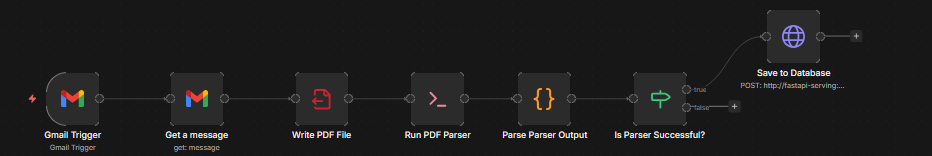
\includegraphics[width=0.92\textwidth]{bab4/Email_PDF_pipeline.png}
\caption{Workflow n8n untuk ingestion formulir kredit PDF melalui email}
\label{fig:bab4_email_pdf_pipeline}
\end{figure}

Skenario kedua adalah pengiriman email konfirmasi kepada pihak yang bertanggung jawab dalam proses persetujuan kredit. Setelah data nasabah dan hasil analisis risiko tersedia, sistem dapat mengirimkan email konfirmasi yang berisi ringkasan informasi pengajuan, hasil penilaian risiko, serta opsi tindak lanjut. Alur ini mendukung proses \textit{human-in-the-loop} karena keputusan akhir tidak sepenuhnya diserahkan kepada model, melainkan tetap dapat ditinjau oleh analis atau pihak berwenang sebelum status persetujuan diperbarui.

\begin{table}[H]
\centering
\caption{Kasus uji konfirmasi email dan keputusan manual}
\label{tab:bab4_email_hitl_test}
\begin{tabular}{|p{0.28\textwidth}|p{0.62\textwidth}|}
\hline
\textbf{Aspek Pengujian} & \textbf{Hasil yang Diharapkan} \\
\hline
Pemicu email & Endpoint \textit{/api/nasabah/\{id\}/send-confirmation} mengirim ringkasan risiko kepada reviewer. \\
\hline
Isi email & Email memuat identitas nasabah, indikator risiko, grade, probabilitas default, serta opsi persetujuan atau penolakan. \\
\hline
Keputusan setuju & Endpoint \textit{/api/nasabah/\{id\}/approve} memperbarui \textit{approval\_status} menjadi \textit{Accepted}. \\
\hline
Keputusan tolak & Endpoint \textit{/api/nasabah/\{id\}/reject} memperbarui \textit{approval\_status} menjadi \textit{Rejected}. \\
\hline
Audit trail & Riwayat pengiriman tercatat pada tabel \textit{sent\_emails}. \\
\hline
\end{tabular}
\end{table}

Selain pengujian alur pengiriman email tunggal, sistem juga mendukung pengiriman notifikasi kepada beberapa staf atau pekerja bank yang terlibat dalam proses peminjaman. Fitur ini menyesuaikan praktik operasional lembaga keuangan, yaitu pengajuan kredit dapat ditinjau oleh lebih dari satu pihak sesuai alur kerja internal, misalnya analis kredit, supervisor, atau pejabat pemutus. Tampilan pengiriman email ke beberapa penerima ditunjukkan pada Gambar \ref{fig:bab4_multiple_email_sent}.

\begin{figure}[H]
\centering
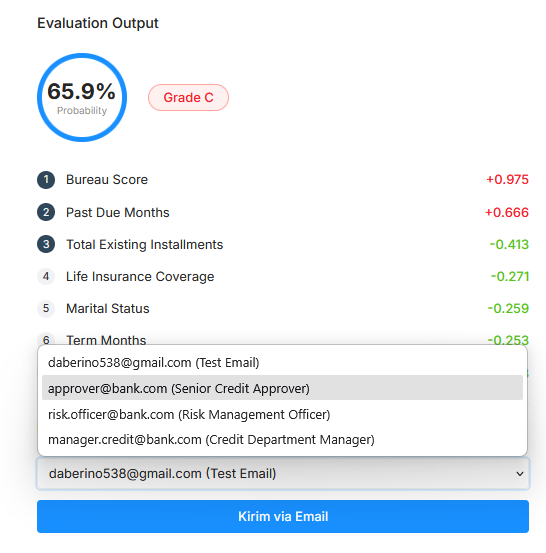
\includegraphics[width=0.80\textwidth]{bab4/MultipleEmailsent.png}
\caption{Pengiriman email konfirmasi ke beberapa staf bank terkait proses persetujuan kredit}
\label{fig:bab4_multiple_email_sent}
\end{figure}

Selain itu, sistem menyediakan formulir peminjaman yang disusun untuk mengikuti kebutuhan data pada proses pengajuan kredit. Formulir tersebut memuat atribut nasabah dan informasi pengajuan yang diperlukan agar data dapat diproses oleh pipeline, disimpan ke database, dan dianalisis oleh model risiko kredit. Tampilan formulir peminjaman ditunjukkan pada Gambar \ref{fig:bab4_form_peminjaman}.

\begin{figure}[H]
\centering
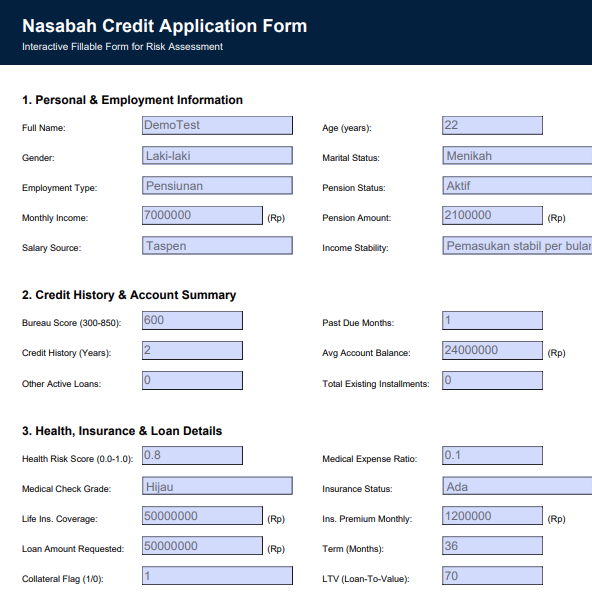
\includegraphics[width=0.92\textwidth]{bab4/FormPeminjaman.png}
\caption{Formulir peminjaman yang digunakan sebagai sumber data pengajuan kredit}
\label{fig:bab4_form_peminjaman}
\end{figure}

\begin{figure}[H]
\centering
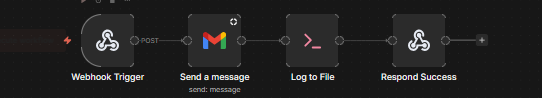
\includegraphics[width=0.92\textwidth]{bab4/Email_Sent_pipeline.png}
\caption{Workflow n8n untuk pengiriman email konfirmasi persetujuan kredit}
\label{fig:bab4_email_sent_pipeline}
\end{figure}

Hasil pengujian kedua workflow tersebut memperlihatkan bahwa n8n berperan sebagai komponen orkestrasi tambahan di luar retraining otomatis. Dengan adanya ingestion PDF dan pengiriman konfirmasi email, pipeline MLOps yang dibangun tidak hanya mencakup pelatihan, serving, dan monitoring model, tetapi juga mendukung integrasi proses bisnis kredit dari penerimaan dokumen hingga eskalasi keputusan kepada manusia.

\subsection{Evaluasi Aturan Bisnis Batas Usia dan Mitigasi Tenor Dinamis}
Sebelum aturan pembatasan usia pelunasan diterapkan pada modul \textit{serving}, sistem evaluasi risiko kredit sepenuhnya bergantung pada keluaran model XGBoost. Kondisi ini menimbulkan celah risiko bisnis karena model dapat meluluskan nasabah berusia lanjut, misalnya berusia 75 hingga lebih dari 80 tahun, dengan peringkat risiko baik dan probabilitas default yang rendah. Anomali tersebut muncul karena sebagian nasabah lanjut usia memiliki profil keuangan yang terlihat kuat bagi model, seperti aliran pendapatan pensiun yang stabil, skor kredit biro yang tinggi, rasio DTI yang rendah, serta status asuransi jiwa aktif.

Kelemahan tersebut menunjukkan bahwa model machine learning murni hanya menangkap korelasi matematis antarfitur, tetapi tidak secara eksplisit memahami risiko biologis dan batas kelayakan usia pelunasan. Sebagai contoh, nasabah berusia 75 tahun dengan profil pensiun stabil dapat dinilai rendah risiko oleh model, walaupun pengajuan tenor 10--15 tahun secara praktis dapat melewati batas usia pelunasan yang aman bagi institusi keuangan. Oleh karena itu, diperlukan lapisan logika bisnis tambahan agar hasil prediksi model tetap selaras dengan kebijakan manajemen risiko.

Untuk mengatasi kondisi tersebut, diterapkan sistem logika hibrida pada lapisan API. Sistem ini menghitung usia saat jatuh tempo dengan Persamaan \ref{eq:bab4_age_maturity}. Jika usia pelunasan melebihi 80 tahun, maka prediksi model dipotong atau \textit{bypass} sehingga sistem tidak memberikan persetujuan otomatis meskipun probabilitas default dari model tergolong rendah.

\begin{equation}
    \text{Usia Pelunasan} = \text{Usia Saat Pengajuan} + \frac{\text{Tenor (Bulan)}}{12}
    \label{eq:bab4_age_maturity}
\end{equation}

Mekanisme mitigasi tersebut dibagi ke dalam \textbf{tiga zona keputusan}:

\begin{enumerate}
    \item \textbf{Zona Lolos Batas Usia} --- kondisi ketika usia pelunasan $\leq$ 80 tahun. Pada zona ini, data tetap dikirimkan ke model XGBoost untuk memperoleh probabilitas \textit{default} dan \textit{risk grade} secara normal.

    \item \textbf{Zona Mitigasi Dinamis} --- kondisi ketika usia nasabah saat pengajuan masih di bawah 80 tahun, tetapi tenor yang diminta menyebabkan usia pelunasan melewati 80 tahun. Pada zona ini, sistem memberikan status Grade Undefined dan menghitung rekomendasi tenor maksimal secara dinamis menggunakan Persamaan \ref{eq:bab4_max_tenor}.

    \begin{equation}
        \text{Tenor Maksimal (Bulan)} = (80 - \text{Usia Saat Pengajuan}) \times 12
        \label{eq:bab4_max_tenor}
    \end{equation}

    Sebagai contoh, nasabah berusia 75 tahun yang mengajukan tenor 120 bulan akan direkomendasikan untuk menurunkan tenor maksimal menjadi 60 bulan. Jika nasabah memiliki asuransi jiwa aktif, sistem juga dapat memberikan rekomendasi dispensasi komite kredit berbasis perlindungan asuransi.

    \item \textbf{Zona \textit{Joint-Borrower}} --- kondisi ketika nasabah telah berusia 80 tahun atau lebih pada saat pengajuan. Pada zona ini, pengurangan tenor tidak lagi memadai karena sisa batas usia bernilai nol atau negatif. Sistem menyarankan alternatif pengajuan berbasis \textit{joint-income} atau \textit{co-borrower} dengan anggota keluarga inti yang lebih muda.
\end{enumerate}

Visualisasi batas keputusan mitigasi ditunjukkan pada Gambar \ref{fig:bab4_mitigation_boundary}. Gambar tersebut memperlihatkan bahwa sistem tidak hanya membedakan nasabah berdasarkan hasil prediksi model, tetapi juga berdasarkan kombinasi usia dan tenor. Area normal menunjukkan pengajuan yang masih dapat dievaluasi oleh model, sedangkan area mitigasi menunjukkan pengajuan yang membutuhkan pengurangan tenor, pertimbangan dispensasi, atau penahanan keputusan otomatis ketika batas usia tidak dapat dipenuhi.

\begin{figure}[H]
\centering
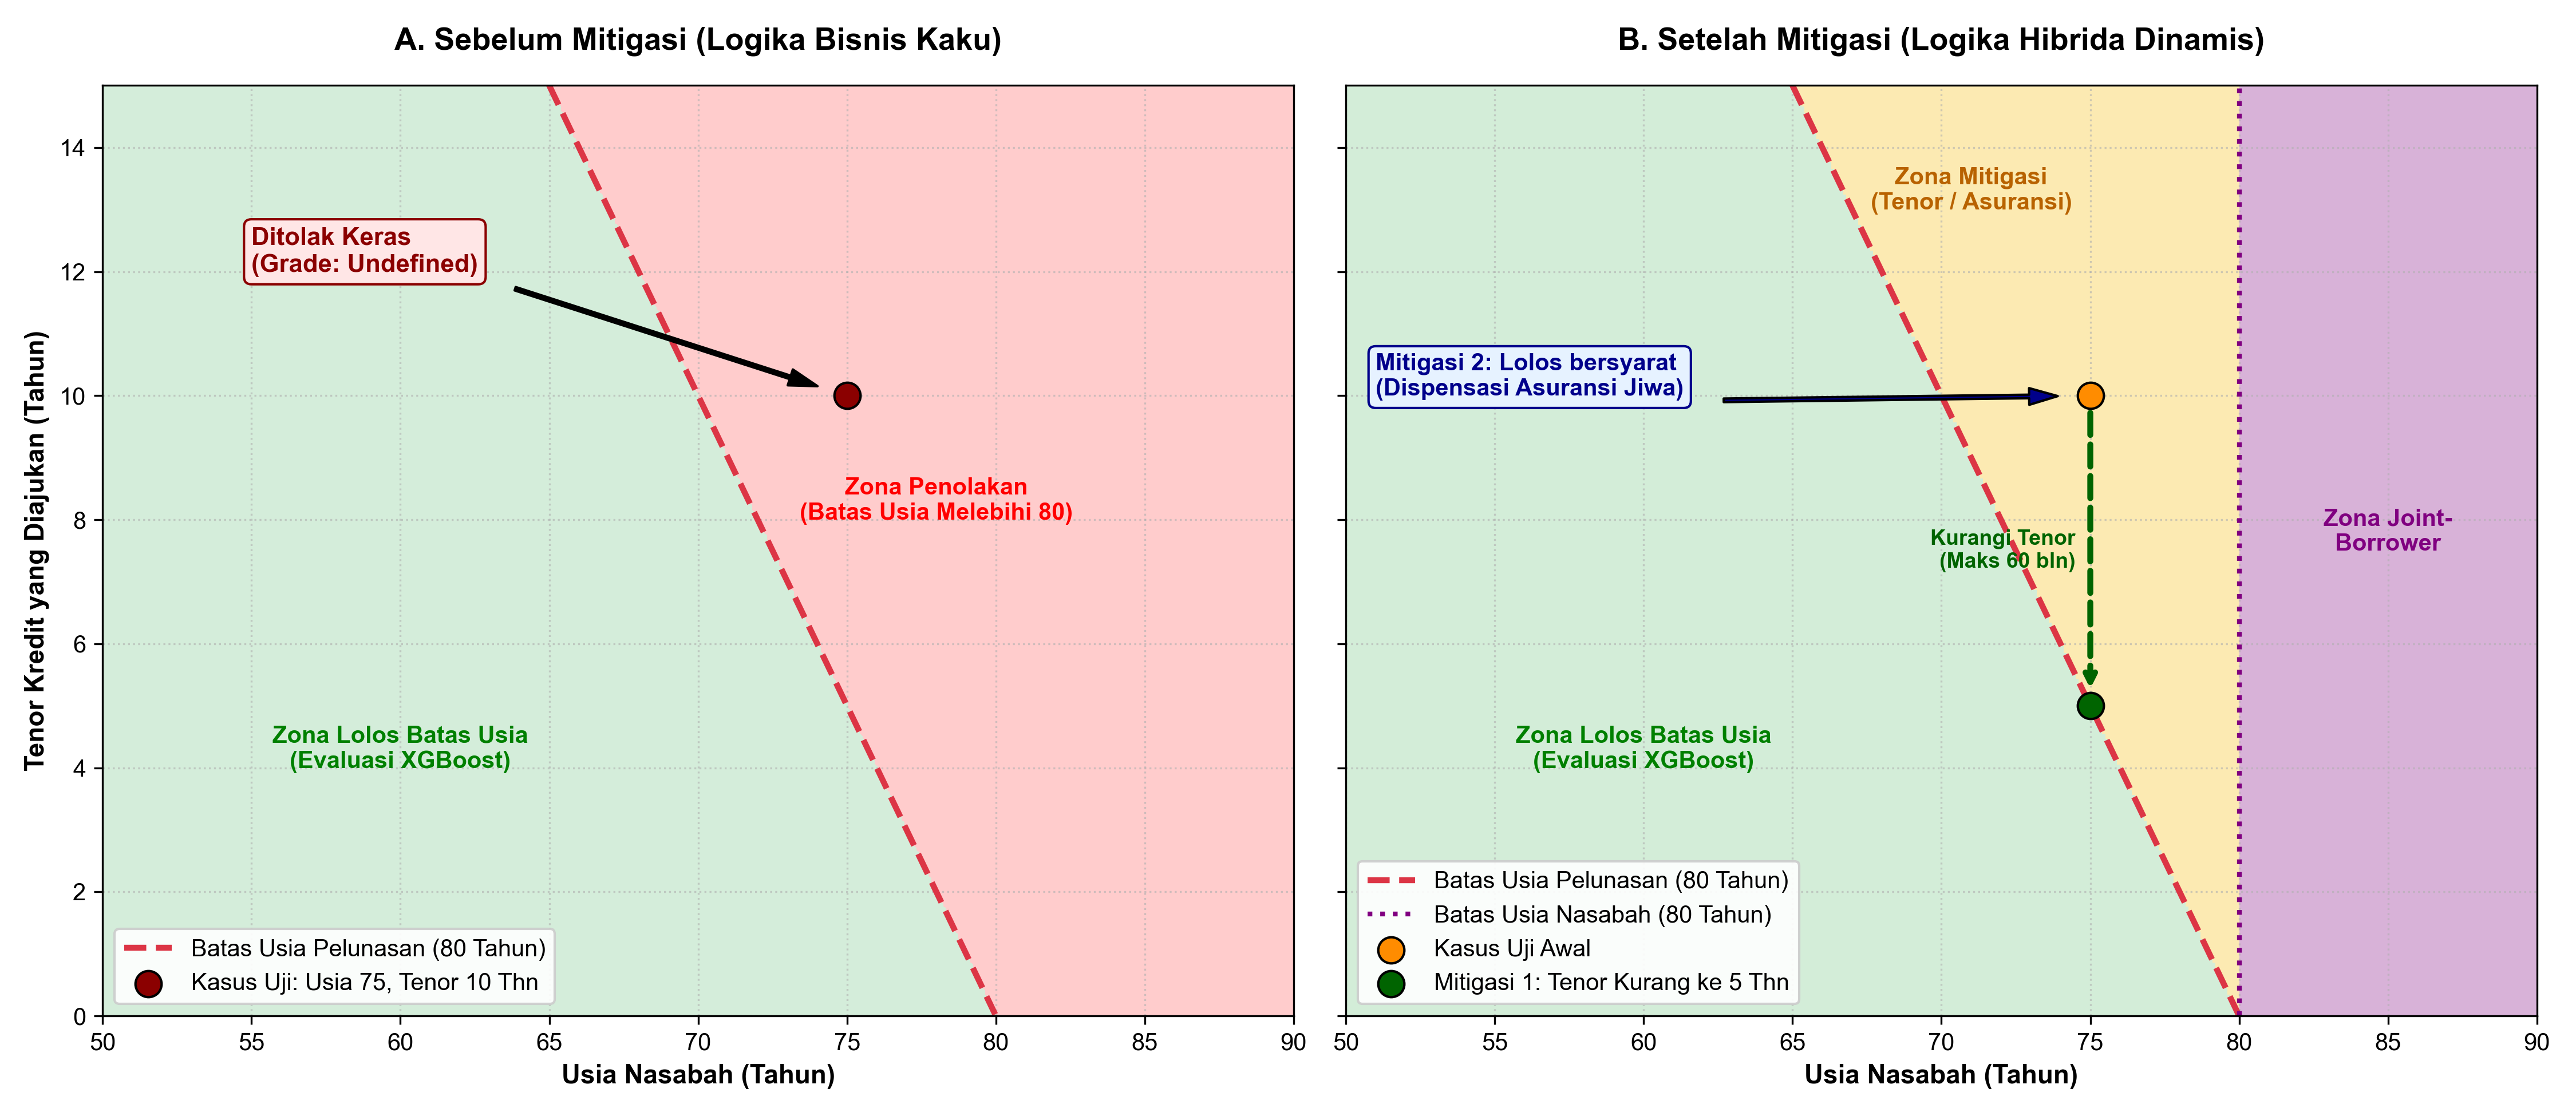
\includegraphics[width=0.82\textwidth]{bab4/mitigation_decision_boundary.png}
\caption{Visualisasi batas keputusan mitigasi usia dan tenor kredit}
\label{fig:bab4_mitigation_boundary}
\end{figure}

Setelah mekanisme ini diterapkan, sistem berhasil menyeimbangkan kecerdasan prediktif model dengan kepatuhan terhadap kebijakan risiko perbankan. Nasabah lanjut usia yang sebelumnya dapat lolos karena profil keuangannya terlihat baik kini terjaring oleh deteksi anomali usia pelunasan. Namun, sistem tidak langsung menolak secara kaku, melainkan memberikan rekomendasi terukur melalui pengurangan tenor atau pertimbangan asuransi jiwa kredit. Dengan demikian, aturan bisnis ini berfungsi sebagai lapisan pengaman tambahan yang membuat hasil inferensi model lebih realistis dan dapat diterapkan pada proses kredit operasional.

\section{Pengujian Deteksi Drift dan Retraining Otomatis}
\label{sec:bab4_drift_retraining}
Pengujian \textit{drift} dilakukan untuk memvalidasi mekanisme pemantauan distribusi data produksi pada modul drift\_monitor.py. Sistem yang dibangun menggunakan pendekatan \textbf{dual-trigger}, yaitu dua jalur pemicuan yang bekerja secara bersamaan: trigger berbasis jadwal setiap 7 hari dan trigger berbasis event saat data nasabah baru diinput. Pengujian difokuskan pada skenario terkontrol untuk membuktikan bahwa kedua mekanisme ini dapat mendeteksi pergeseran distribusi dan secara otomatis memicu proses retraining melalui webhook n8n.

\subsection{Pengujian Trigger Berbasis Jadwal}

Pada jalur ini, sistem secara terjadwal membandingkan distribusi fitur data produksi terkini terhadap distribusi data referensi menggunakan \textbf{Kolmogorov-Smirnov (KS) Test}. KS Test dipilih karena merupakan uji distribusi non-parametrik yang tidak memerlukan asumsi distribusi tertentu sehingga cocok untuk fitur tabular dengan distribusi campuran.

Skenario \textbf{stabil} dibandingkan dengan skenario \textbf{drift} yang mensimulasikan penurunan pendapatan sebesar 20\% dan peningkatan jumlah pinjaman sebesar 35\%, merepresentasikan kondisi makroekonomi yang memburuk. Hasil pengujian ditampilkan pada Tabel~\ref{tab:bab4_drift}.

\begin{table}[H]
\centering
\caption{Hasil pengujian deteksi drift menggunakan KS Statistic}
\label{tab:bab4_drift}
\begin{tabular}{|p{0.22\textwidth}|p{0.16\textwidth}|p{0.16\textwidth}|p{0.14\textwidth}|p{0.18\textwidth}|}
\hline
\textbf{Fitur} & \textbf{KS Stabil} & \textbf{KS Drifted} & \textbf{p-value} & \textbf{Tindakan} \\
\hline
\textit{monthly\_income} & 0,043 & 0,312 & $< 0{,}05$ & Webhook retrain dipicu \\
\hline
\textit{loan\_amount} & 0,038 & 0,287 & $< 0{,}05$ & Webhook retrain dipicu \\
\hline
\end{tabular}
\end{table}

Pada kondisi stabil, nilai KS-statistic kedua fitur berada di bawah 0,05 dengan \textit{p-value} $> 0{,}05$, menunjukkan bahwa distribusi produksi tidak berbeda signifikan dari distribusi referensi --- layanan API tetap berjalan normal. Pada kondisi drifted, nilai KS-statistic melonjak melampaui ambang signifikansi $\alpha = 0{,}05$, sehingga sistem mengklasifikasikan kondisi sebagai \textit{drift terdeteksi} dan mengeksekusi fungsi trigger\_retrain untuk mengirim \textit{HTTP POST} ke server n8n.

\subsection{Pengujian Trigger Berbasis Event}

Jalur kedua bekerja secara independen. Setiap kali endpoint POST /api/nasabah menerima data nasabah baru, sistem menambah penghitung kumulatif data baru sejak model terakhir dilatih. Apabila penghitung melampaui \textit{ingestion threshold} yang dikonfigurasi, \textit{workflow} n8n memicu evaluasi dan retraining secara langsung tanpa menunggu jadwal mingguan.

Hal ini menunjukkan bahwa pipeline MLOps mampu membentuk mekanisme \textit{closed-loop automation}: model tidak hanya digunakan untuk inferensi, tetapi juga dipantau dan diperbarui secara responsif --- baik oleh perubahan distribusi data (schedule trigger) maupun oleh volume data baru yang masuk (event trigger).

Implementasi orkestrasi retraining otomatis pada n8n ditunjukkan pada Gambar \ref{fig:bab4_n8n_workflow}. Workflow tersebut memuat beberapa komponen utama, yaitu \textit{Schedule Trigger} untuk eksekusi berkala, \textit{Webhook} untuk menerima pemicu eksternal dari modul drift monitoring, node eksekusi perintah untuk menjalankan proses pemeriksaan atau pelatihan ulang, node kondisional untuk menentukan apakah retraining diperlukan, serta \textit{HTTP Request} untuk menghubungkan proses otomasi dengan layanan terkait. Dengan struktur tersebut, proses monitoring dan retraining dapat dijalankan secara otomatis tanpa intervensi manual penuh.

\begin{figure}[H]
\centering
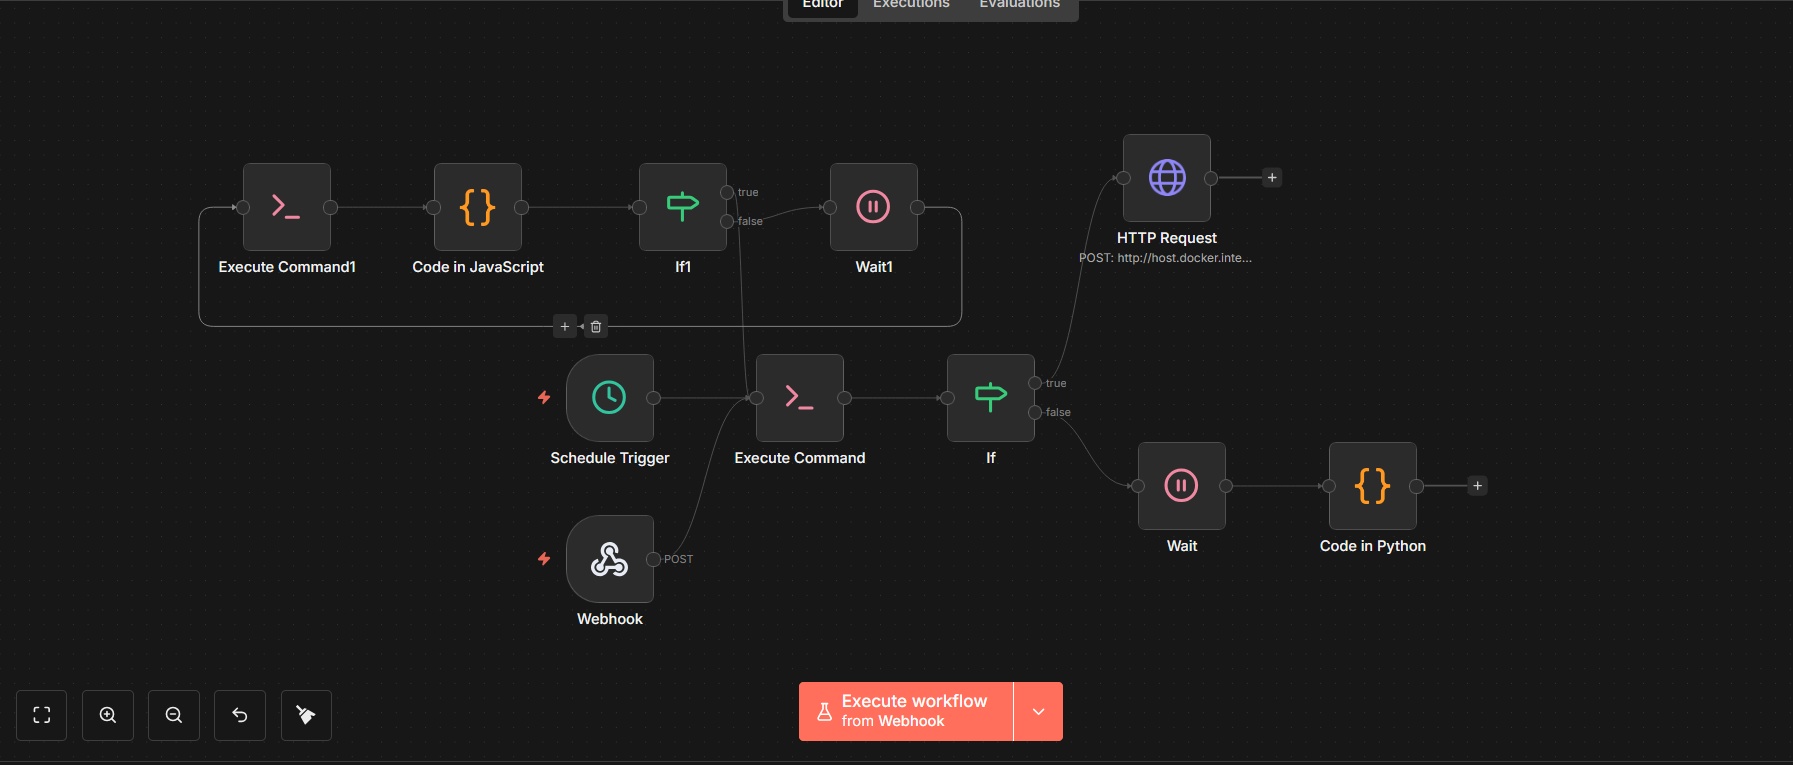
\includegraphics[width=0.92\textwidth]{bab4/Screenshot 2026-05-25 171559.png}
\caption{Workflow n8n untuk orkestrasi monitoring drift dan retraining otomatis}
\label{fig:bab4_n8n_workflow}
\end{figure}

\section{Analisis Deskriptif}
\label{sec:bab4_evaluasi_kritis}
Meskipun hasil pengujian menunjukkan bahwa pipeline MLOps telah mampu menjalankan otomasi pelatihan, deployment, monitoring drift, dan integrasi aturan bisnis, sistem ini masih memiliki beberapa batasan jika dilihat dari sudut pandang manajemen risiko riil. Evaluasi kritis ini penting karena sistem penilaian kredit tidak hanya harus akurat secara teknis, tetapi juga harus aman secara operasional dan dapat dipertanggungjawabkan secara ekonomi.

\subsection{Kebutuhan Human-in-the-Loop pada Zona Ambang}
Meskipun sistem telah memiliki mekanisme konfirmasi email untuk mendukung \textit{human-in-the-loop}, pengujian pada zona ambang tetap membutuhkan aturan eskalasi yang lebih eksplisit. Pada nilai probabilitas gagal bayar atau \textit{Probability of Default} (PD) yang berada pada zona ambang, misalnya 40\% hingga 60\%, tingkat ketidakpastian model relatif tinggi. Jika kasus pada rentang ini tidak secara otomatis diberi tanda \textit{mandatory human review}, maka sistem tetap berpotensi menghasilkan kesalahan klasifikasi, baik berupa \textit{false positive} maupun \textit{false negative}.

Dalam praktik operasional perbankan, zona abu-abu tersebut sebaiknya tidak diperlakukan sebagai keputusan otomatis. Mekanisme email yang telah tersedia perlu diperkuat dengan \textit{review flag} berbasis threshold agar pengajuan pada zona ambang otomatis dialihkan kepada analis kredit atau \textit{credit underwriter}. Dengan demikian, hasil prediksi model dapat dikombinasikan dengan penilaian kualitatif, seperti stabilitas pekerjaan, kondisi keluarga, dokumen pendukung, dan informasi tambahan yang tidak selalu tercermin di dalam fitur model.

\subsection{Beban Finansial Spesifik yang Tidak Sepenuhnya Tercermin pada Risk Grade}
Berdasarkan penelaahan deskriptif terhadap sampel data nasabah, terdapat celah antara validasi lapangan dan keluaran model. Sebagai contoh, pada sampel nasabah di Tabel \ref{tab:nasabah_normal}, terdapat nasabah dengan pendapatan bulanan sekitar Rp3.285.278 dan rasio pengeluaran medis yang tinggi. Jika rasio pengeluaran medis mencapai 42,09\%, maka sekitar Rp1,38 juta per bulan digunakan untuk biaya medis rutin. Secara operasional, beban tersebut dapat bertindak sebagai \textit{fixed commitment} yang mengurangi kapasitas membayar atau \textit{repayment capacity}.

Kondisi serupa juga dapat terjadi pada pengeluaran non-medis yang bersifat mengikat, seperti biaya pendidikan anak berkebutuhan khusus atau kewajiban keluarga lain yang tidak selalu tertangkap secara eksplisit oleh model. Dalam beberapa kasus, model masih dapat memberikan grade yang relatif moderat karena didorong oleh fitur lain seperti \textit{bureau\_score} yang tinggi. Hal ini menunjukkan bahwa catatan manual dari petugas Kredit Validator tetap perlu menjadi bagian dari proses intervensi, terutama ketika terdapat beban finansial spesifik yang tidak cukup direpresentasikan oleh variabel model.

Dengan demikian, keluaran model sebaiknya diposisikan sebagai alat bantu keputusan, bukan pengganti penuh proses validasi kredit. Pipeline perlu dikembangkan agar dapat menerima \textit{manual override flag} atau catatan validator sebagai sinyal tambahan untuk menurunkan grade, mengubah status menjadi Undefined, atau mengalihkan kasus ke proses review manual.

\subsection{Kerentanan Subjektivitas pada Proses WoE Binning}
Transformasi \textit{Weight of Evidence} (WoE) terbukti membantu stabilitas fitur dan mendukung interpretabilitas model. Namun, proses pembentukan interval atau \textit{binning} pada variabel numerik tetap memiliki unsur sensitivitas metodologis. Perbedaan metode binning, seperti \textit{equal width}, \textit{equal frequency}, atau binning berbasis aturan bisnis, dapat menghasilkan batas interval yang berbeda dan pada akhirnya mengubah nilai WoE.

Jika batas bin ditentukan semata-mata oleh algoritma tanpa validasi dari komite risiko, model dapat menjadi benar secara teknis tetapi kurang tepat secara ekonomi. Sebagai contoh, perubahan kecil pada batas kelompok \textit{bureau\_score} dapat mengubah interpretasi risiko dan memengaruhi skor akhir nasabah. Oleh karena itu, proses binning perlu divalidasi tidak hanya berdasarkan metrik statistik, tetapi juga berdasarkan kewajaran bisnis dan kebijakan risiko lembaga keuangan.

Batasan ini menunjukkan bahwa implementasi pipeline MLOps pada domain kredit perlu dilengkapi dengan tata kelola model yang kuat. Setiap perubahan fitur, binning WoE, threshold PD, aturan grading, dan mekanisme retraining sebaiknya terdokumentasi, ditinjau, dan disetujui oleh pihak yang bertanggung jawab terhadap risiko model.

\subsection{Dependensi Infrastruktur pada Lingkungan Lokal}
Pengujian sistem dilakukan pada lingkungan lokal menggunakan Docker dan Docker Compose. Konfigurasi ini memadai untuk validasi prototipe karena seluruh komponen seperti FastAPI, MLflow, n8n, database SQLite, dan file log dapat dijalankan dalam satu lingkungan pengujian. Namun, untuk skenario produksi skala penuh, ketergantungan pada konektivitas lokal antarservice dan penyimpanan file lokal perlu diperhatikan karena dapat menjadi titik kegagalan ketika jumlah pengguna, volume prediksi, atau kebutuhan audit meningkat.

Pada implementasi produksi, database SQLite dapat dipertimbangkan untuk dimigrasikan ke sistem basis data server seperti PostgreSQL, sedangkan log inferensi sebaiknya disimpan pada penyimpanan terpusat atau terdistribusi. Selain itu, komunikasi antarservice perlu dilengkapi autentikasi, pemantauan ketersediaan, serta strategi backup dan recovery. Dengan demikian, sistem tidak hanya siap secara fungsional, tetapi juga lebih kuat dari sisi reliabilitas dan tata kelola operasional.

\section{Ringkasan Bab}
\label{sec:bab4_ringkasan}
Bab ini telah menguraikan hasil pengujian sistem mulai dari preprocessing, penanganan imbalance, pelatihan model, evaluasi performa, interpretabilitas, quality gate data sintetis, API serving, database nasabah, ingestion PDF, konfirmasi email HITL, aturan bisnis, hingga deteksi drift. Hasil pengujian menunjukkan bahwa model XGBoost memperoleh AUC 0,8262 dengan keseimbangan presisi dan recall yang baik. Transformasi WoE dan seleksi IV membantu memperkuat dasar pemilihan fitur, sedangkan SHAP memberikan transparansi terhadap faktor yang memengaruhi prediksi.

Selain performa model, hasil pengujian juga menunjukkan bahwa data sintetis lolos quality gate utilitas dan privasi, layanan FastAPI mampu mengembalikan prediksi beserta penjelasan, database mendukung CRUD dan audit email, workflow n8n mendukung retraining serta ingestion PDF, aturan bisnis dapat mencegah keputusan yang melanggar kebijakan, dan sistem drift monitoring mampu memicu retraining otomatis. Dengan demikian, sistem yang dikembangkan tidak hanya memenuhi kebutuhan pemodelan prediktif, tetapi juga menunjukkan kesiapan sebagai pipeline MLOps yang operasional, dapat diaudit, dan tetap membutuhkan tata kelola manusia pada kasus yang berisiko.
